\documentclass[12pt]{article}
\usepackage[utf8]{inputenc}
\usepackage[english,russian]{babel}
\usepackage[table,xcdraw]{xcolor}
\usepackage{graphicx}
\usepackage{float}
\usepackage{amsmath}
\usepackage{amssymb}
\usepackage[a4paper,top=3cm,bottom=2cm,left=2.5cm,right=2.5cm,marginparwidth=1.75cm]{geometry}
\usepackage[unicode, pdftex]{hyperref}
\usepackage{titlesec}
\titleformat{\section}
    {\normalfont\fontsize{12}{15}\bfseries}{\thesection}{1em}{}
\usepackage{gensymb}
\usepackage{titlesec}
\usepackage{gensymb}
\usepackage{listings}
\usepackage{csquotes}
\usepackage{caption}
\usepackage{framed}
\usepackage{tabularx}
\usepackage{subcaption}
\usepackage[linesnumbered,ruled,vlined]{algorithm2e}
\usepackage{siunitx}
\sisetup{
    round-mode=places,
    round-precision=3,
    scientific-notation=true,
    table-number-alignment = center,
}

\usepackage[format=plain,justification=centering]{caption}

\usepackage[symbol*]{footmisc}

\usepackage{tikz-uml}

\setfnsymbol{wiley}
\newcommand\mycommfont[1]{\footnotesize\ttfamily\textcolor{blue}{#1}}
\SetCommentSty{mycommfont}

\SetKwInput{KwInput}{Input}                % Set the Input
\SetKwInput{KwOutput}{Output}              % set the Output

\def\t{\texttt}

\titleformat{\section}  % which section command to format
  {\fontsize{18}{10}\bfseries} % format for whole line
  {\thesection)} % how to show number
  {1em} % space between number and text
  {} % formatting for just the text
  [] % formatting for after the text

\titleformat{\subsection}  % which section command to format
  {\fontsize{14}{10}\bfseries} % format for whole line
  {\thesubsection)} % how to show number
  {1em} % space between number and text
  {} % formatting for just the text
  [] % formatting for after the text


\newcommand\bigo{\mathcal{O}}

\begin{document}

\begin{titlepage}
\begin{center}

\large Федеральное государственное автономное образовательное учреждение высшего образования\\
\Large{\textbf{Национальный исследовательский университет}}\\
\begin{figure}[H]
    \centering
    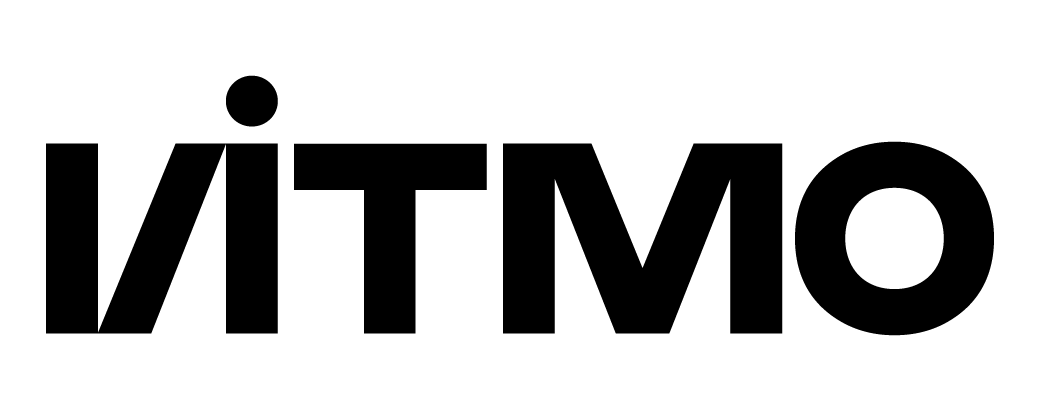
\includegraphics[width=0.3\linewidth]{label.png}
\end{figure}
\vspace{0.5cm}
\large Факультет информационных технологий и программирования\\

\vspace{1.5cm}

\textbf{\fontsize{60pt}{0}\selectfont{ОТЧЕТ}}\\
\vspace{0.5cm}
по лабораторной работе №4\\
\vspace{0.5cm}
на тему:\\
\vspace{0.5cm}
\textbf{\enquote{Сопряженные направления и методы Ньютона}}


\begin{flushright}
Работу выполнили студенты\\
Группы M3233\\
Калиновский Арсений Владимирович\\
Рудаков Максим Андреевич\\
\end{flushright}
    
\includegraphics[width=.76\linewidth]{image.png}
\vfill


Санкт-Петербург\\  
\today


\end{center}
\end{titlepage}

\section{Цели работы}
Самостоятельная реализация и изучение методов сопряжённых градиентов, методов Ньютона и квазиньютоновских методов, а также их сравнение с библиотечной реализацией метода NewtonCG, на примере их работы на квадратичных функциях различной обусловленности и сложных функциях, в том числе:
\begin{itemize}
    \item Эффективность работы,
    \item Особенности поведения при различных конфигурациях,
    \item Характера сходимости,
    \item Вычислительных потребностей.
\end{itemize}

\section{Задачи, решаемые при выполнении работы}
\begin{itemize}
    \item Реализация алгоритмов оптимизации,
    \item Получение экспериментальных данных (таблицы, графики) для различных конфигураций работы алгоритма,
    \item Изучение особенностей работы алгоритмов на основании полученных экспериментальных данных.
\end{itemize}

\section{Объект исследования}
Оптимизаторы многомерных функций, реализованных с использованием методов сопряжённых градиентов, методов Ньютона и квазиньютоновских методов.

\section{Модели задач}
\begin{itemize}
    \item Квадратичные функции различной размерности и степени обусловленности,
    \item Функция Розенброка (сложная функция),
    \item Функция Химмельблау (сложная функция).
\end{itemize}

\section{Структура проекта}

\section{Структура проекта}
Проект состоит из 3 частей:
\begin{enumerate}
    \item Модуль \t{optimizers}, в котором содержится реализация всех оптимизаторов,
    \item Файлы \t{functions.py} и \t{quadratic.py}, в котором содержатся описания функций, использованных в рамках исследовательской работы,
    \item Функция $\t{main}$, которая отвечает за вызов оптимизаторов, сбор данных и введение статистики (таблицы, графики).
\end{enumerate}

Иерархия оптимизаторов схематически изображена на рисунке ниже:

\begin{center}
\resizebox{\textwidth}{!}{
\begin{tikzpicture}
\umlabstract[x=0, y=10]{BaseOptimizer}{\text{Статистика, утилиты}}{
    \t{@abstractmethod} \\
    \t{def \_iteration(self)}
}

\umlabstract[x=-8, y=6]{QuasiNewton}{
\t{\_sk, \_yk}
}{
    \t{@abstractmethod} \\
    \t{def \_calculate\_pk(self)}
} \umlabstract[x=-10.3, y=2.6]{DenseQuasiNewton}{
    \t{\_Gk} 
}{
    \t{@abstractmethod} \\
    \t{def \_calculate\_Gk\_impl()}
} \umlclass[x=-12, y=0]{BFGS}{}{} \umlclass[x=-8, y=0]{DFP}{}{} \umlclass[x=-6, y=3]{LBFGS}{}{}

\umlclass[x=-8, y=10]{LinearConjugateGradient}{}{}

\umlabstract[x=0, y=6]{NonLinearConjugateGradient}{
    \t{\_gk\_prev, \_pk}
}{
    \t{@abstractmethod} \\
    \t{def \_calculate\_beta()}
} \umlclass[x=-2, y=1]{FletcherReeves}{}{} \umlclass[x=2, y=1]{PolakRibiere}{}{}

\umlabstract[x=7, y=6]{Ньютоновские методы}{}{} \umlabstract[x=12, y=6]{Trust-region методы}{}{} 

\umlclass[x=5.5, y=3]{NewtonDirection}{}{} \umlclass[x=8, y=0]{NewtonCholesky}{}{} \umlclass[x=10, y=3]{NewtonCG}{}{} 

\umlclass[x=12, y=0]{PowellsDogLeg}{}{}

\umlinherit{QuasiNewton}{BaseOptimizer} \umlinherit{LinearConjugateGradient}{BaseOptimizer} \umlinherit{Ньютоновские методы}{BaseOptimizer} \umlinherit{Trust-region методы}{BaseOptimizer} 

\umlinherit{NewtonCG}{Ньютоновские методы} \umlinherit{NewtonDirection}{Ньютоновские методы} \umlinherit{NewtonCholesky}{Ньютоновские методы} 

\umlinherit{PowellsDogLeg}{Trust-region методы} 

\umlinherit{DenseQuasiNewton}{QuasiNewton} \umlinherit{LBFGS}{QuasiNewton} \umlinherit{BFGS}{DenseQuasiNewton} \umlinherit{DFP}{DenseQuasiNewton}

\umlinherit{NonLinearConjugateGradient}{BaseOptimizer} \umlinherit{FletcherReeves}{NonLinearConjugateGradient} \umlinherit{PolakRibiere}{NonLinearConjugateGradient}
\end{tikzpicture} 
}
\captionof{figure}{Иерархия классов оптимизационных методов}
\end{center}
Результаты выполнения функции $\t{main}$ распределены в зависимости от задания по разным папкам, которые имеют названия $\t{task1-4}$. В названии каждого файла явно указаны метод и оптимизируемая функция, а также некоторая дополнительная информация, которая может иметь значение для конкретного задания (папка $\t{task4}$ дополнительная; в ней содержатся экспериментальные данные для анализа L-BFGS).

В рамках лабораторной работы в качестве условия остановки использовалось условие на норму градиента: $\nabla f_k < \varepsilon$, где $\varepsilon = 10^{-8}$.

\section {Оптимизируемые функции}
В данном разделе будут приведены определения оптимизируемых функций.
\subsection{Квадратичные функции}
В рамках этой лабораторной работы использовались случайно сгенерированные квадратичные функции. Квадратичная функция имеет вид:
\begin{equation*}
f(\textbf{x}) = \frac12\langle \textbf{x}, A\textbf{x} \rangle + \langle b, \textbf{x} \rangle + c
\end{equation*}

Заметим, что $A = H_f$ --- гессиан квадратичной функции.

Для генерации функции использовались 2 параметра:
\begin{itemize}
    \item $n$ --- размерность пространства,
    \item $k$ --- число обусловленности гессиана $A$.
\end{itemize}

Для генерации квадратичных функций используется следующий алгоритм:

\begin{algorithm}[H]
\DontPrintSemicolon
    \KwInput{$n, k$}
    \KwOutput{Quadratic function $f\;:\;\mathbb{R}^n \rightarrow \mathbb{R}$}

    Generate $\lambda_{\min}$ \reflectbox{$\mapsto$} $x / n, x \sim \mathcal{U}_{[0,1]}$\;
    $\lambda_{\max}$ \reflectbox{$\mapsto$} $k \cdot \lambda_{\min}$\;
    Generate $(\lambda_1,\ldots,\lambda_n)$ \reflectbox{$\mapsto$} $\textbf{x} \sim \mathcal{U}_{[\lambda_{\min}, \lambda_{\max}]}^n$\;

    Choose $i,j \in \{1,\ldots,n\}$\;

    $\lambda_i\ \reflectbox{$\mapsto$}\ \lambda_{\min}$\;
    $\lambda_j\ \reflectbox{$\mapsto$}\ \lambda_{\max}$\;

    $\Lambda$ \reflectbox{$\mapsto$} $\operatorname{diag}(\lambda_1,\ldots,\lambda_n)$\;

    Generate $\textbf{v}$ \reflectbox{$\mapsto$} $(1 / n^2) \cdot \textbf{x}, \textbf{x} \sim \mathcal{N}(0,1)^n$\;

    $Q$ \reflectbox{$\mapsto$} $I - 2\textbf{v}\textbf{v}^T$\;

    $A$ \reflectbox{$\mapsto$} $Q^T \Lambda Q$\;

    Generate $\textbf{x}^*$ \reflectbox{$\mapsto$} $\textbf{x} \sim \mathcal{N}(0,1)^n$\;

    $b$ \reflectbox{$\mapsto$} $A \textbf{x}^*$\;

    $c$ \reflectbox{$\mapsto$} $\mathcal{U}_{[0,1]}$\;

    \Return{$A,b,c,\textbf{x}^*$}
\caption{Генерация случайной квадратичной функции}
\end{algorithm}

Обратим внимание на деление на $n$ и $n^2$ в строчках 1, 8. Оно делается для стабилизации матрицы: без деления значения матрицы быстро возрастут до порядка тысяч, из-за чего во многих опытах найти оптимальное значение не получится из-за огромных значений функции и градиента.

\subsection{Сложные функции}

В рамках данной лабораторной работы использованы следующие \enquote{сложные функции}:
\begin{itemize}
    \item Функция Розенброка $\rho(x,y) = (1 - x)^2 + 100(y - x^2)^2$. У неё единственный минимум 0 в точке (1,1). Заметим, что функция Розенброка не является выпуклой. Её градиент $\nabla \rho$ имеет вид $(-2(1 - x) - 400 x (y - x ^2), 200 (y - x^2))$. Её гессиан $H_{\rho}$ имеет вид:
    \begin{equation*}
        H_{\rho} = \left(
        \begin{array}{cc}
            2 - 400y + 1200x^2 & -400x \\
            -400x & 200
        \end{array}
        \right)
    \end{equation*}
    \begin{figure}[H]
        \centering
        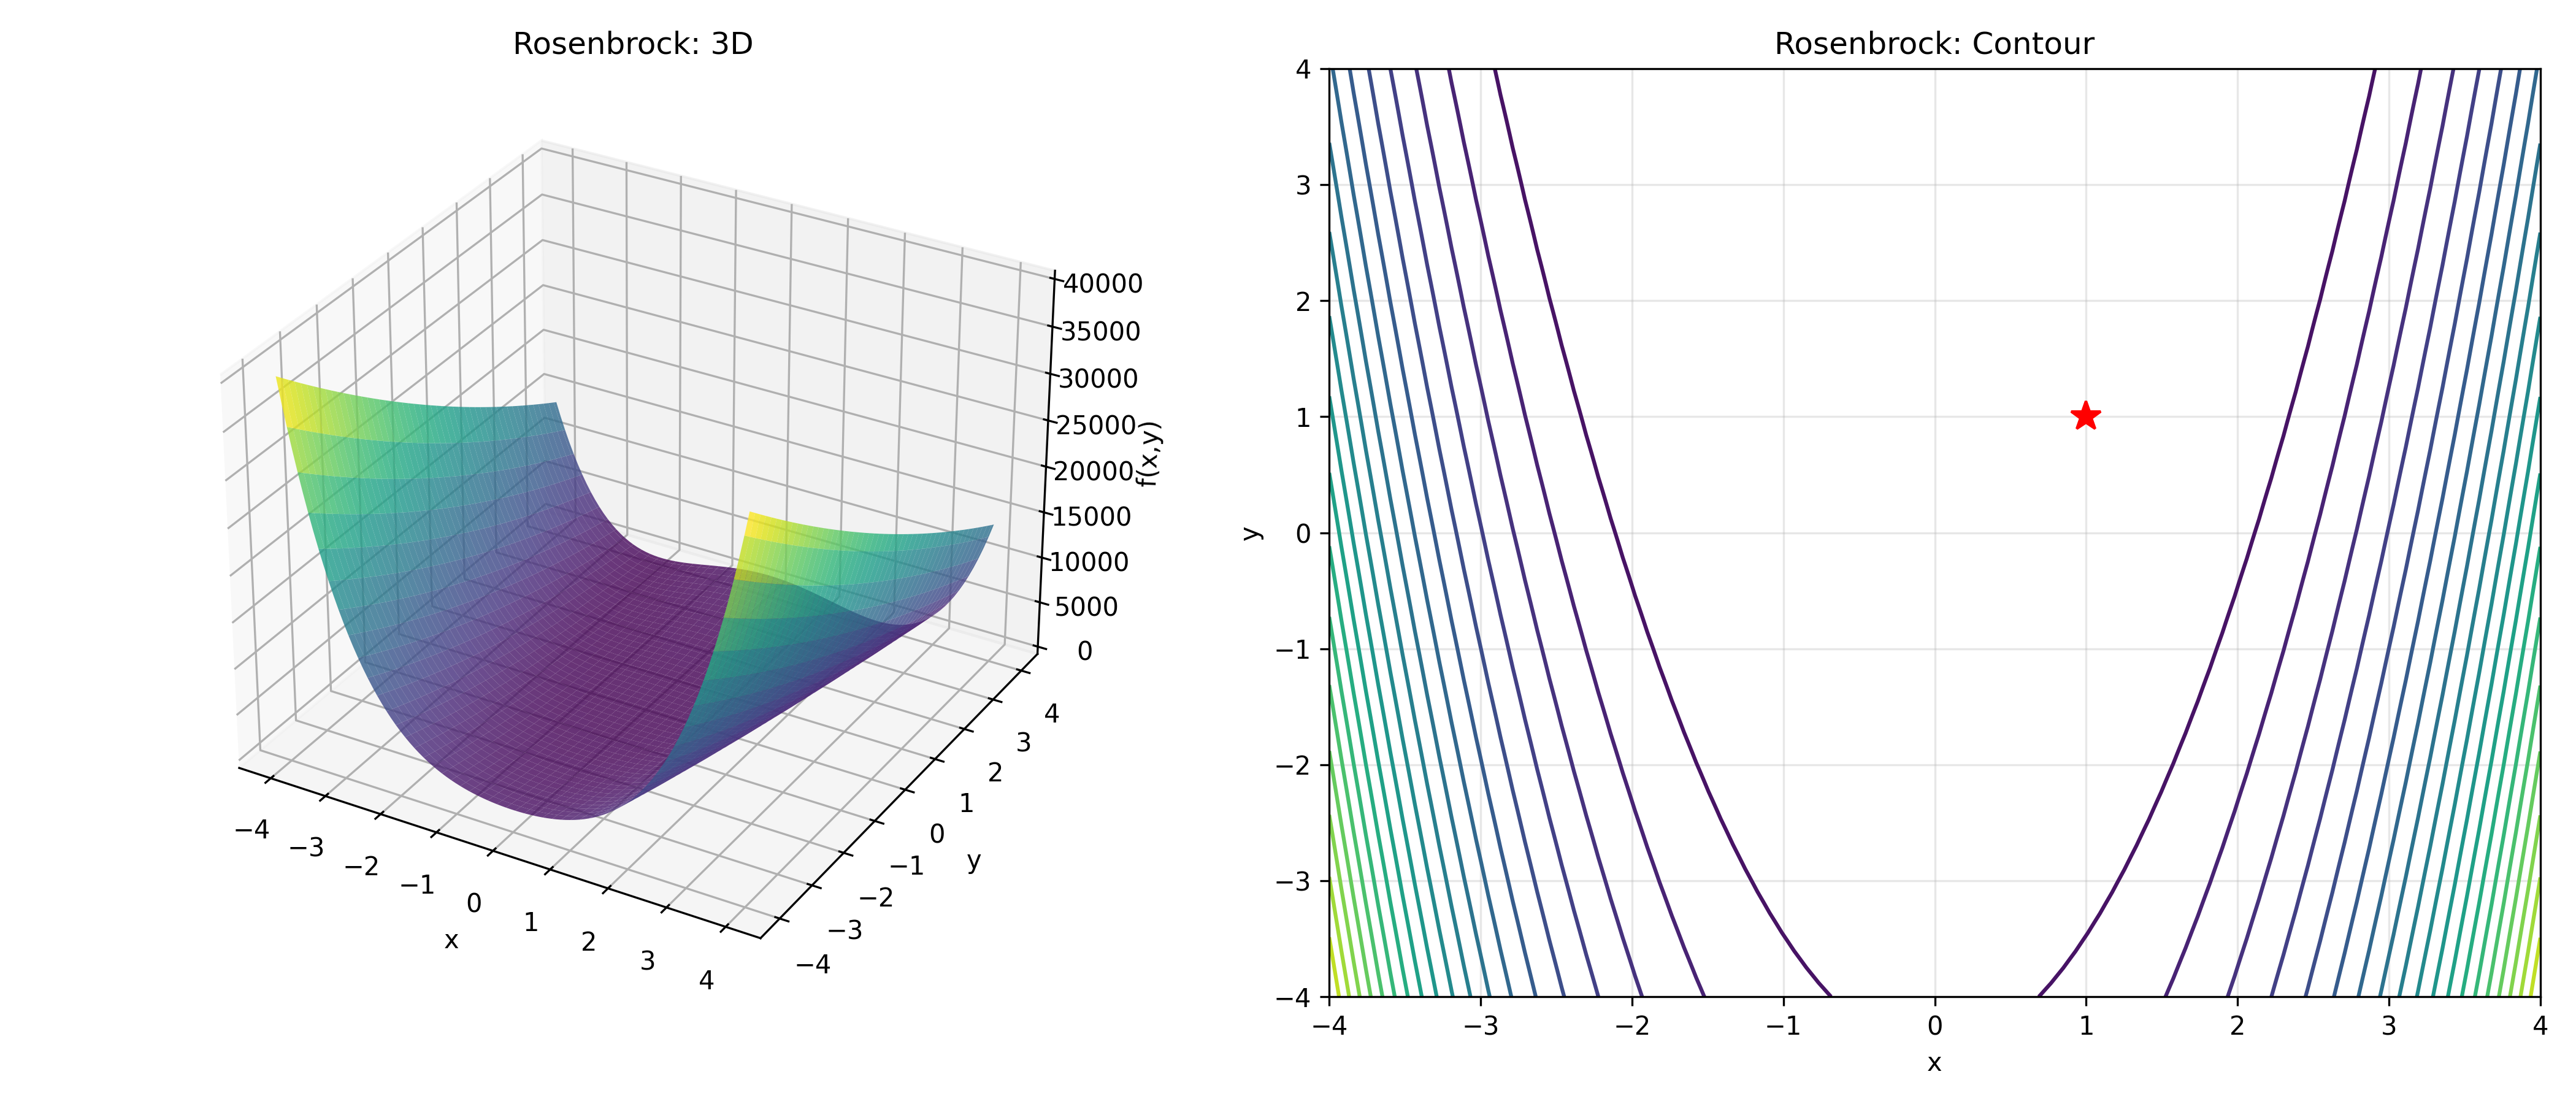
\includegraphics[width=.8\linewidth]{rosenbrock.png}
        \caption{График функции Розенброка.}
    \end{figure}
    \item Функция Химмельблау, равная $\xi (x, y) = (x ^ 2 + y - 11)^2 + (x + y^2 -y)^2$. Эта функция характеризуется наличием трёх равнозначных локальных минимумов, в каждом из которых функция принимает значение 0. Эти минимумы соответственно имеют вид (3,2), (-2.805$\ldots$, 3.131$\ldots), (-3.779$\ldots, -3.283$\ldots$), (3.584$\ldots$, -1.848$\ldots$). Её градиент имеет вид:
    \begin{equation*}
        \nabla \xi (x, y) = \left(
        \begin{array}{c}
            4ax + 2b \\
            2a + 4by
        \end{array}
        \right),
    \end{equation*}
    \begin{equation*}
        a = x^2 + y - 11, b = x + y^2 - 7.
    \end{equation*}
    Её гессиан $H_{\xi}$ имеет вид:
    \begin{equation*}
        H_{\xi} = \left(
        \begin{array}{cc}
            4a + 8x^2 + 2 & 4(x + y) \\
            4(x + y) & 4b + 8y^2 + 2
        \end{array}
        \right),
    \end{equation*}
    \begin{equation*}
        a = x^2 + y - 11, b = x + y^2 - 7.
    \end{equation*}
    \begin{figure}[H]
        \centering
        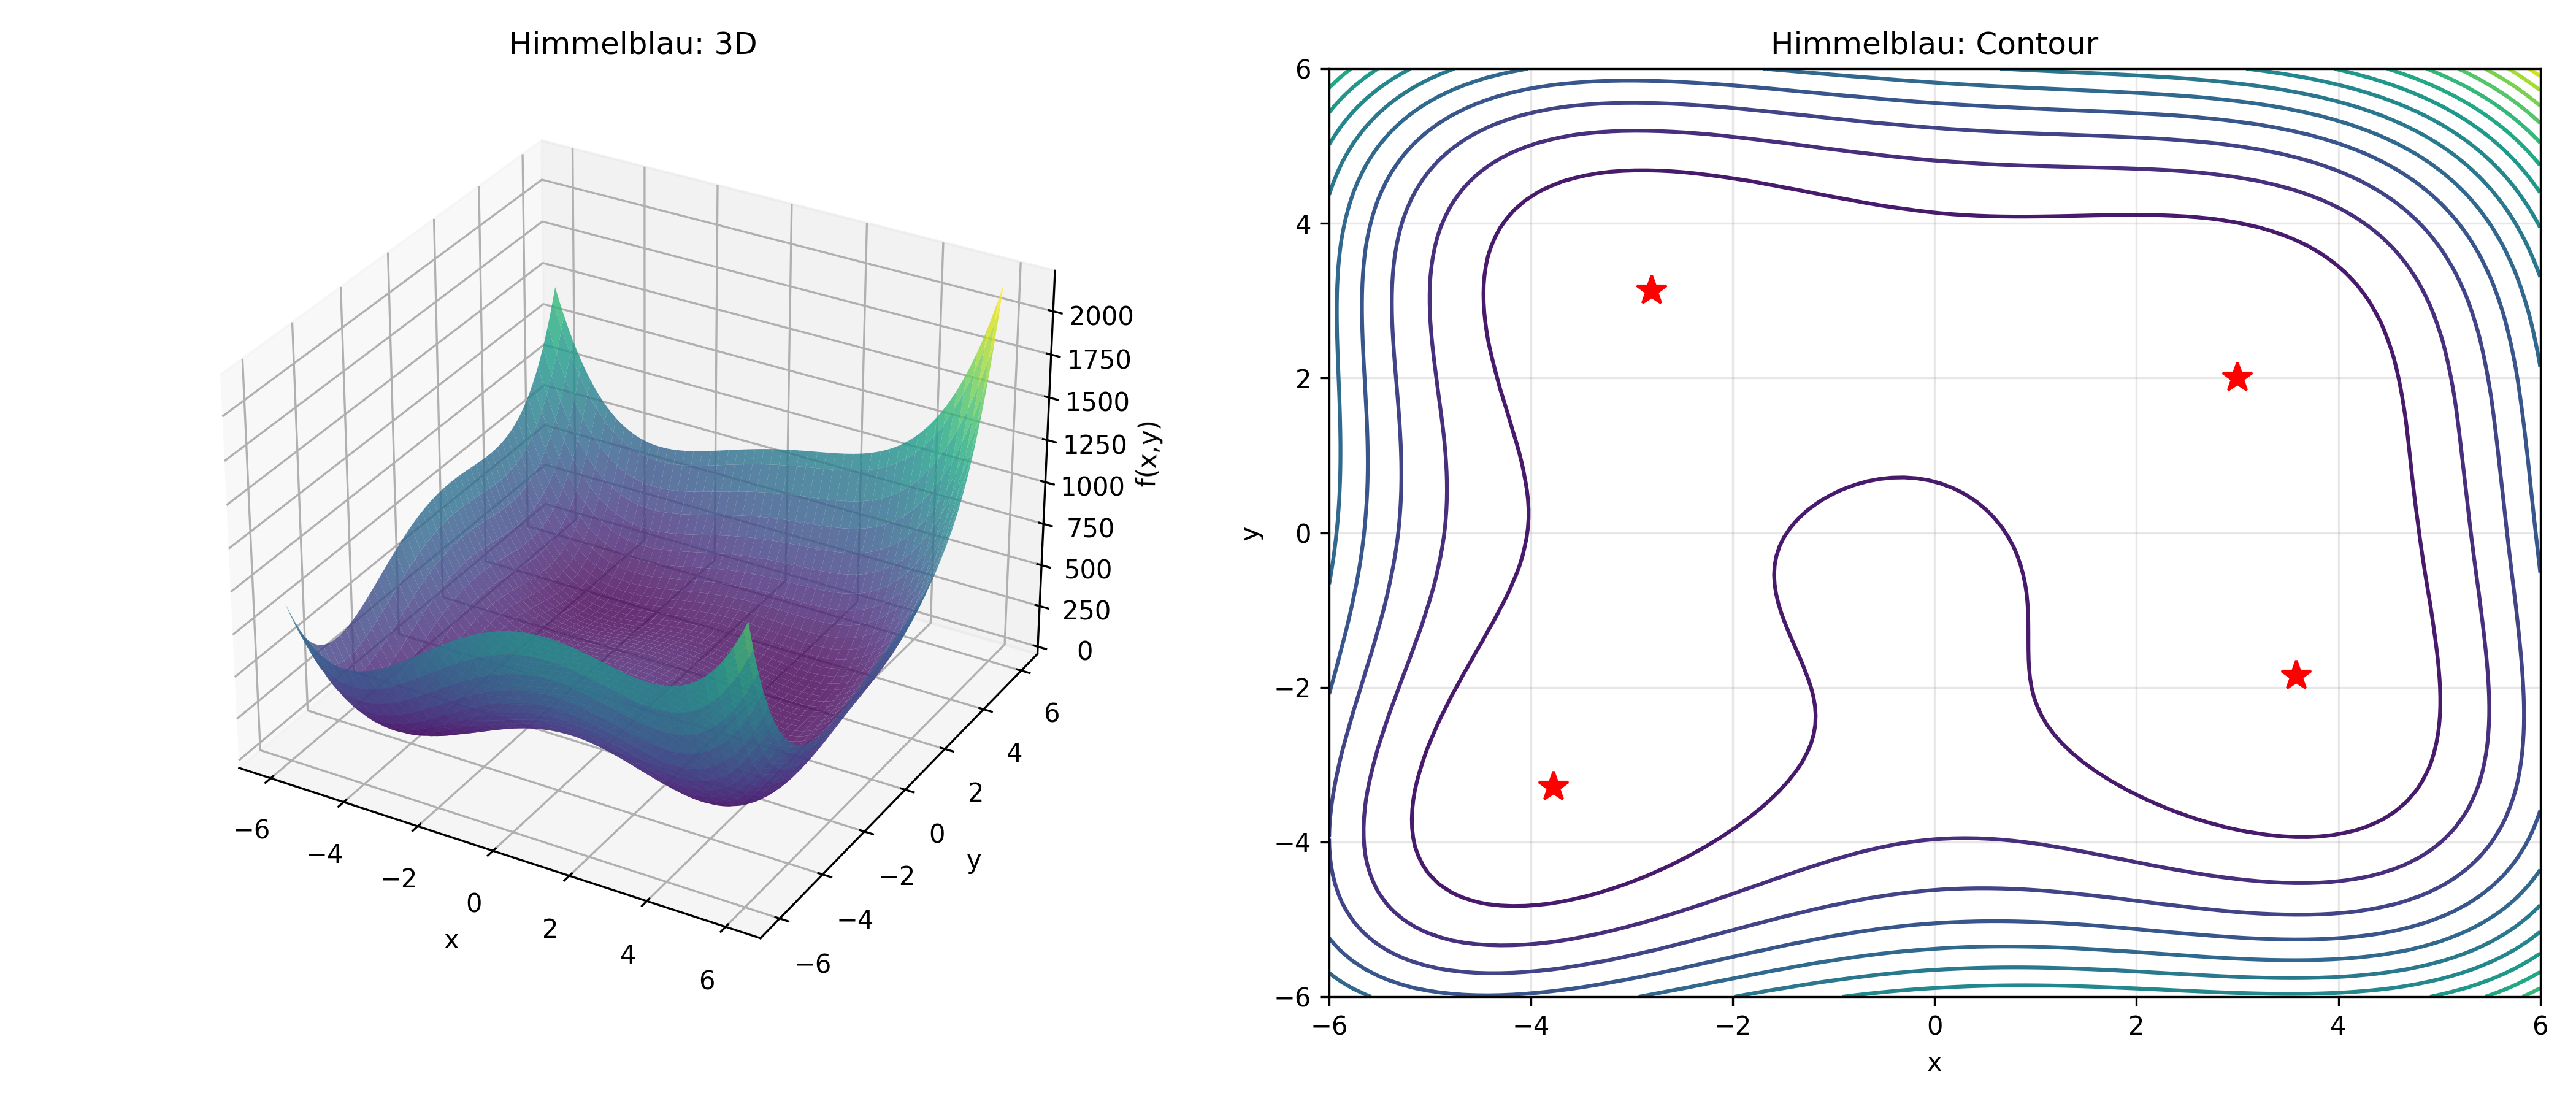
\includegraphics[width=1\linewidth]{himmelblau.png}
        \caption{График функции Химмельблау}
    \end{figure}
\end{itemize}

\section{Теория}

Пусть имеется многомерная функция $f : D \subseteq \mathbb{R}^n \rightarrow \mathbb{R}$, у которой есть точка минимума $\textbf{x}^*$. Заметим, что итерационный процесс можно описать последовательностью $\{\textbf{x}_k\}_{i=1}^{\infty}$, в которой $\textbf{x}_{k+1} = \textbf{x}_k - \alpha_k p_k$, где $\alpha_k$ -- скаляр, а $p_k$ -- вектор. Таким образом, для нахождения минимума достаточно найти такие $\alpha_k, p_k$, что последовательность векторов $\textbf{x}_k$ сходится к точке минимума функции.

Метод сопряженных коэффициентов заключается в выборе $\alpha_k = \frac{\|g_k \|^2}{\langle Ap_k,p_k\rangle}, g_k = \nabla f(\textbf{x}_k)$, $p_0 = g_0$, $p_{k+1} = g_{k+1} + \beta_k p_k$, где $\beta_k = \frac{\|g_{k+1} \|^2}{\|g_k \|^2}$. В теории данный метод должен сходиться не более чем за $n$ итераций для квадратичных функций, однако для плохо обусловленных функций ввиду вычислительных ошибок фактическое число итераций может различаться.

Нелинейный метод сопряженных градиентов заключается в выборе $\beta_k^{\text{FR}} = \frac{\|g_{k+1} \|^2}{\|g_k \|^2}$ (формула Флетчера-Ривса) либо $\beta_k^{\text{PR}} = \frac{\langle g_{k+1}, g_{k+1} - g_k\rangle}{\|g_k \|^2}$ (формула Полака-Рибьера). Число $\alpha_k$ можно выбирать по разному; в рамках данной лабораторной работы $\alpha_k$ выбиралось таким образом, чтобы соблюдались сильные условия Вольфе, либо, если нельзя найти такое $\alpha_k$, равным 1.

Метод Ньютона заключается в выборе в качестве вектора $p_k$ \textit{ньютоновское направление}, которое определяется равенством $H_k p_k = g_k$, где $H_k = H_f(\textbf{x}_k)$. Направление шага $\alpha_k$ можно выбирать по-разному, например, так, чтобы соблюдалось условие Армихо. Таким образом, вычисление направления шага подразумевает нахождение решения уравнения $H_k p_k = g_k$. Сделать это можно, например, разложив гессиан в произведение нижнетреугольной матрциы $L$ и её транспонирования. После решаются уравнения $Lz = g_k, L^Tp_k = z$. Если разложение не удалось (например, потому что гессиан не положительно определенный), то можно в качестве направления выбрать направление градиентного спуска. В этом заключается метод Ньютона с выбором направления.

Метод Powell's Dog Leg заключается в построении квадратичной модели функции и решении trust region подзадачи. В качестве шага выбирается либо ньютоновское направление, либо направление градиентного спуска, либо их взвешенная сумма. При этом на каждой итерации сравнивается предсказанное и фактическое убывания, после чего радиус доверительной области либо уменьшается, если модель плохо предсказала функцию, либо не меняется или увеличивается, если предсказание оказалось хорошим.

Квазиньютоновские методы похожи на ньютоновские методы, однако они вместо прямого вычисления гессиана ищут лишь его приближение (или, что чаще, приближение обратной к гессиану матрицы). При этом должно выполняться \textit{секущее условие}: $G_{k+1} y_k = s_k$, где $y_k = \Delta g_k$, $s_k = \Delta \textbf{x}_k$. В рамках лабораторной работы исследованы подходы BFGS и DFP.

Формула BFGS имеет вид:
\begin{equation*}
    G_{k+1}^{\text{BFGS}} = (I - \rho_k s_k y_k^T)G_k(I - \rho_k y_k s_k^T) + \rho_k s_k s_k^T, \rho_k = \frac{1}{\langle y_k, s_k \rangle}.
\end{equation*}

Формула DFP для матрицы $G_k$ имеет вид:
\begin{equation*}
    G_{k+1}^{\text{DFP}} = G_k + \rho_k s_k s_k^T - \frac{G_k y_k y_k^T G_k}{\langle y_k, G_k y_k\rangle}.
\end{equation*}

Метод L-BFGS похож на метод BFGS, с той разницей, что приближение обратного гессиана не хранится напрямую, а вычисляется приблизительно, с использованием информации о $m$ предыдущих шагах. Таким образом, требуется не $\bigo(n^2)$, а лишь $\bigo(mn)$ памяти.

\section{Анализ результатов}
\subsection{Сходимость для квадратичных функций при различных конфигурациях}

Здесь в качестве начальной позиции использовалась точка (5,5,...) (вектор из одних \enquote{пятёрок}).

\begin{itemize}
    \item Для метода сопряжённых градиентов заметим, что при увеличении параметра $n$ или $k$ график начинает всё больше походить на линейную зависимость. Тем не менее, на многих графиках с фиксированными $k$ видно, что число итераций больше, чем размерность пространства. Это обусловлено накапливающимися ошибками вычислений.
    \begin{figure}[H]
    \centering
    \subcaptionbox{Зависимость от $n$ ($k = 3^8$)}{
\includegraphics[width=0.5\textwidth]{task1_LinearConjugateGradient_fix_k_6561.png}}%
    \subcaptionbox{Зависимость от $k$ ($n = 2^9$)}{
\includegraphics[width=0.5\textwidth]{task1_LinearConjugateGradient_fix_n_512.png}}%
    \caption{Метод сопряжённых коэффициентов при различных конфигурациях.}
    \end{figure}
    \item Методы Флетчера-Ривса и Полака-Рибьера ведут себя схоже: при увеличении параметра $k$ зависимость от $n$ дестабилизируется; при этом при фиксированном параметре $n$ число вызовов функции возрастает от $k$ хаотичным образом.
    \begin{figure}[H]
    \centering
    \subcaptionbox{Зависимость от $n$ ($k = 3^8$)}{
\includegraphics[width=0.5\textwidth]{task1_FletcherReeves_fix_k_6561.png}}%
    \subcaptionbox{Зависимость от $k$ ($n = 2^9$)}{
\includegraphics[width=0.5\textwidth]{task1_FletcherReeves_fix_n_512.png}}%
    \caption{Метод Флетчера-Ривса при различных конфигурациях.}
    \end{figure}
    \begin{figure}[H]
    \centering
    \subcaptionbox{Зависимость от $n$ ($k = 3^8$)}{
\includegraphics[width=0.5\textwidth]{task1_PolakRibiere_fix_k_6561.png}}%
    \subcaptionbox{Зависимость от $k$ ($n = 2^9$)}{
\includegraphics[width=0.5\textwidth]{task1_PolakRibiere_fix_n_512.png}}%
    \caption{Метод Полака-Рибьера при различных конфигурациях.}
    \end{figure}
    \item Метод Ньютона с использованием разложения Холецкого и метод Ньютона с выбором направления работают относительно стабильно, выполняя поиск минимума не более, чем за 16 шагов. При этом число итераций, вызовов градиента и вызовов гессиана незначительно колеблются от константного значения.
    \begin{figure}[H]
    \centering
    \subcaptionbox{Зависимость от $n$ ($k = 3^8$)}{
\includegraphics[width=0.4\textwidth]{task1_NewtonCholesky_fix_k_6561.png}}%
    \subcaptionbox{Зависимость от $k$ ($n = 2^9$)}{
\includegraphics[width=0.4\textwidth]{task1_NewtonCholesky_fix_n_512.png}}%
    \caption{Метод Ньютона с использованием разложения Холецкого при различных конфигурациях.}
    \end{figure}
    \begin{figure}[H]
    \centering
    \subcaptionbox{Зависимость от $n$ ($k = 3^8$)}{
\includegraphics[width=0.4\textwidth]{task1_NewtonDirection_fix_k_6561.png}}%
    \subcaptionbox{Зависимость от $k$ ($n = 2^9$)}{
\includegraphics[width=0.4\textwidth]{task1_NewtonDirection_fix_n_512.png}}%
    \caption{Метод Ньютона с выбором направления при различных конфигурациях.}
    \end{figure}
    \item Метод Powell's Dog Leg работает стабильно. При этом, количество итераций при фиксированном $k$ зависит от числа итераций как логарифм размерности пространства. Про конкретный вид функциональной зависимости числа итераций от числа обусловленности судить сложно, но можно предположить, что она существует.
    \begin{figure}[H]
    \centering
    \subcaptionbox{Зависимость от $n$ ($k = 3^8$)}{
\includegraphics[width=0.5\textwidth]{task1_PowellsDogLeg_fix_k_6561.png}}%
    \subcaptionbox{Зависимость от $k$ ($n = 2^9$)}{
\includegraphics[width=0.5\textwidth]{task1_PowellsDogLeg_fix_n_512.png}}%
    \caption{Метод Powell's Dog Leg при различных конфигурациях.}
    \end{figure}
    \item Про методы BFGS и DFP нельзя ничего особого сказать, кроме того, что при возрастании $n$, $k$ число итераций для нахождения минимума возрастает, причём при увеличении $n$ или $k$ графики зависимости начинают выглядит всё более хаотичными.
    \begin{figure}[H]
    \centering
    \subcaptionbox{Зависимость от $n$ ($k = 3^8$)}{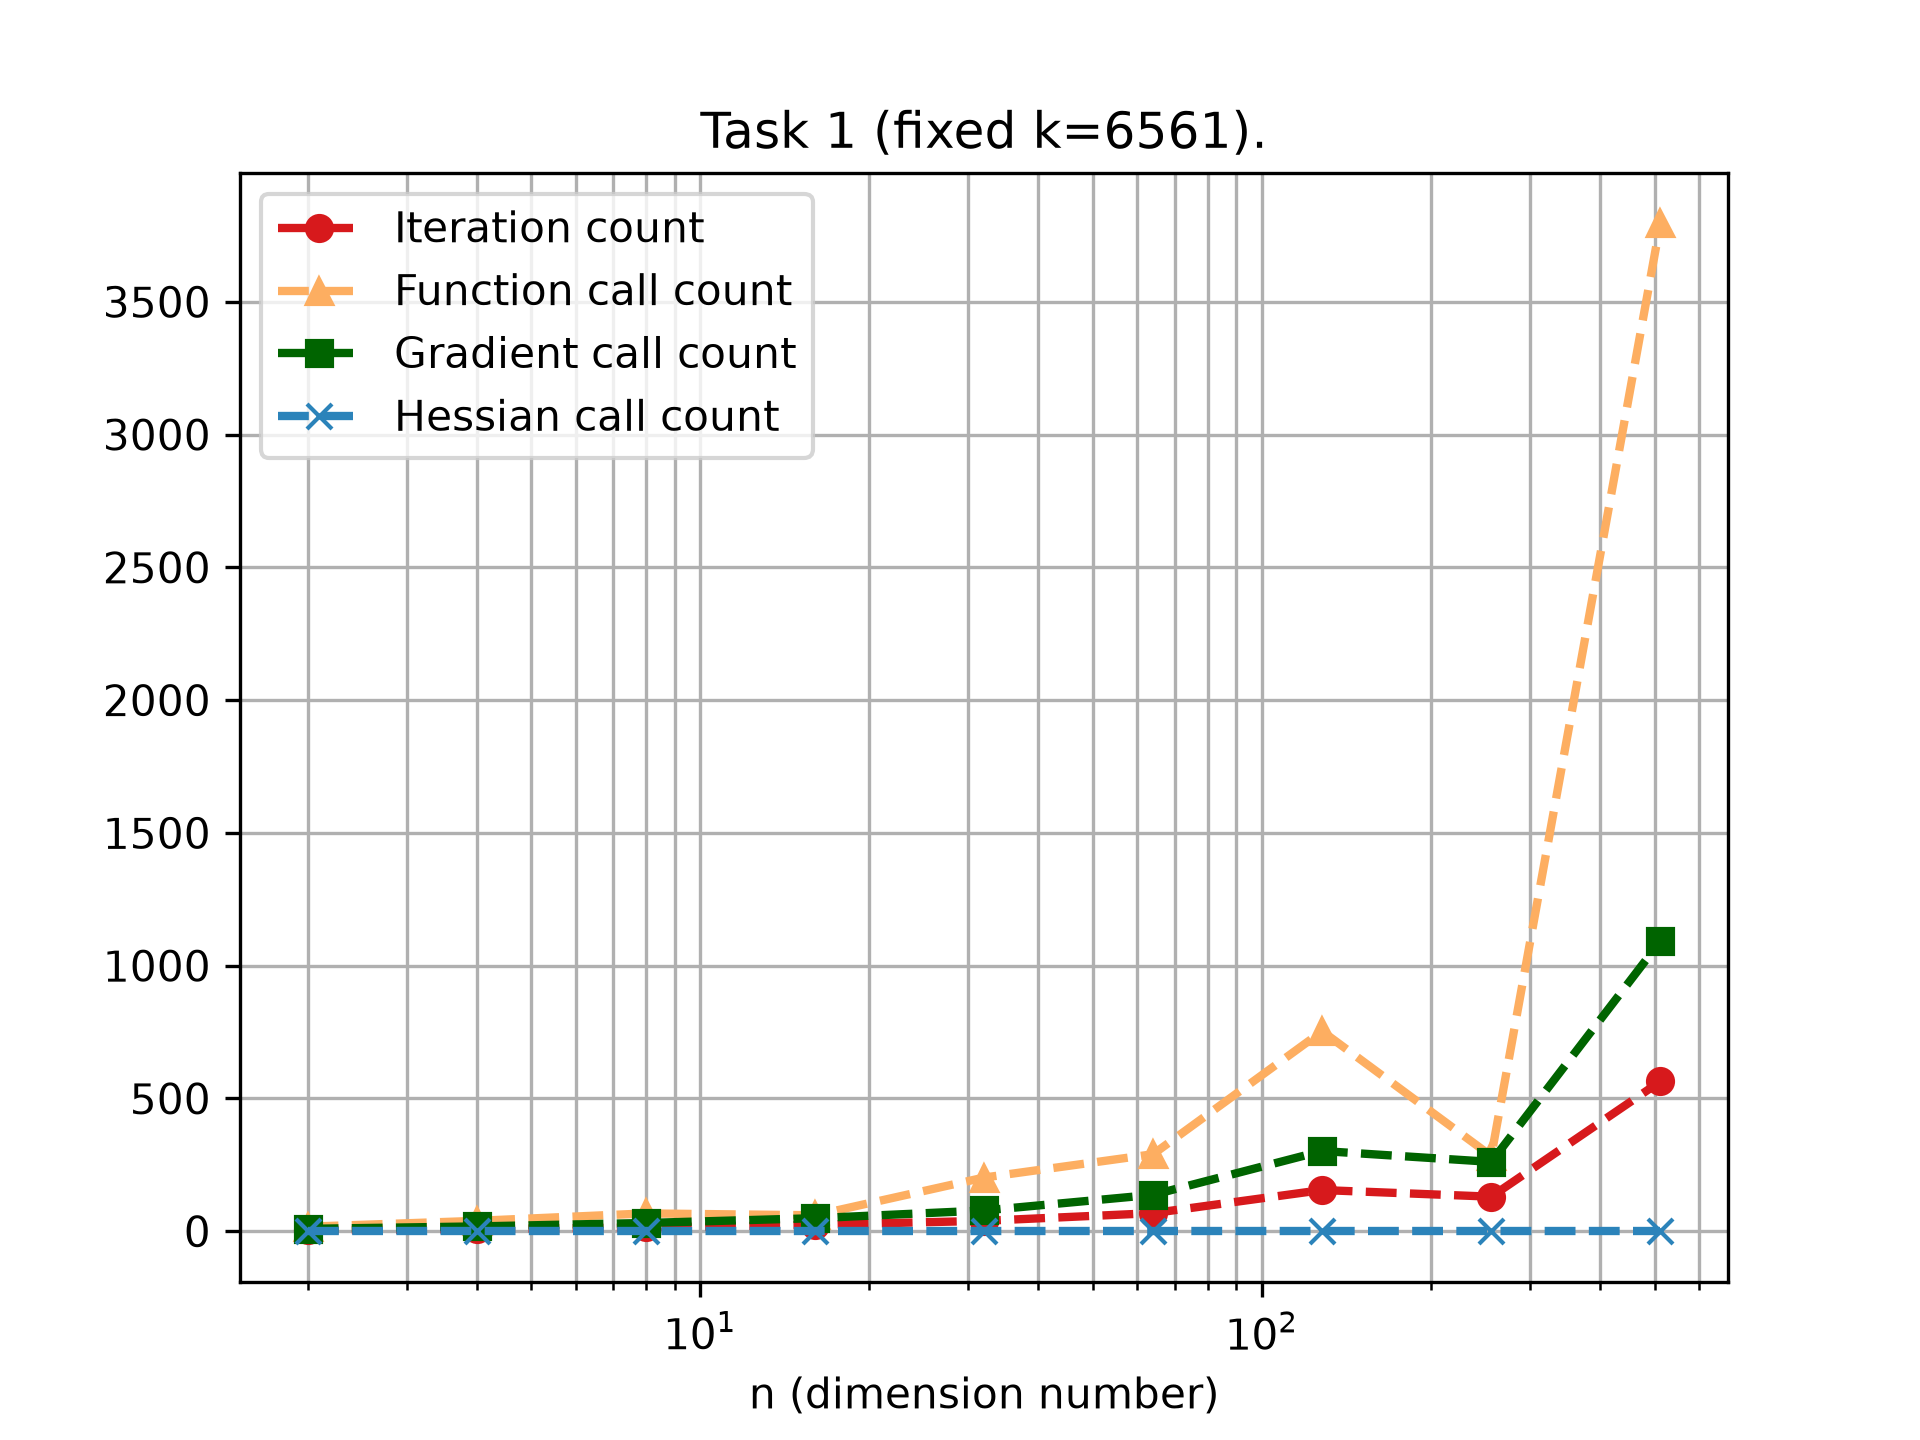
\includegraphics[width=0.5\textwidth]{task1_BFGS_fix_k_6561.png}}%
    \subcaptionbox{Зависимость от $k$ ($n = 2^9$)}{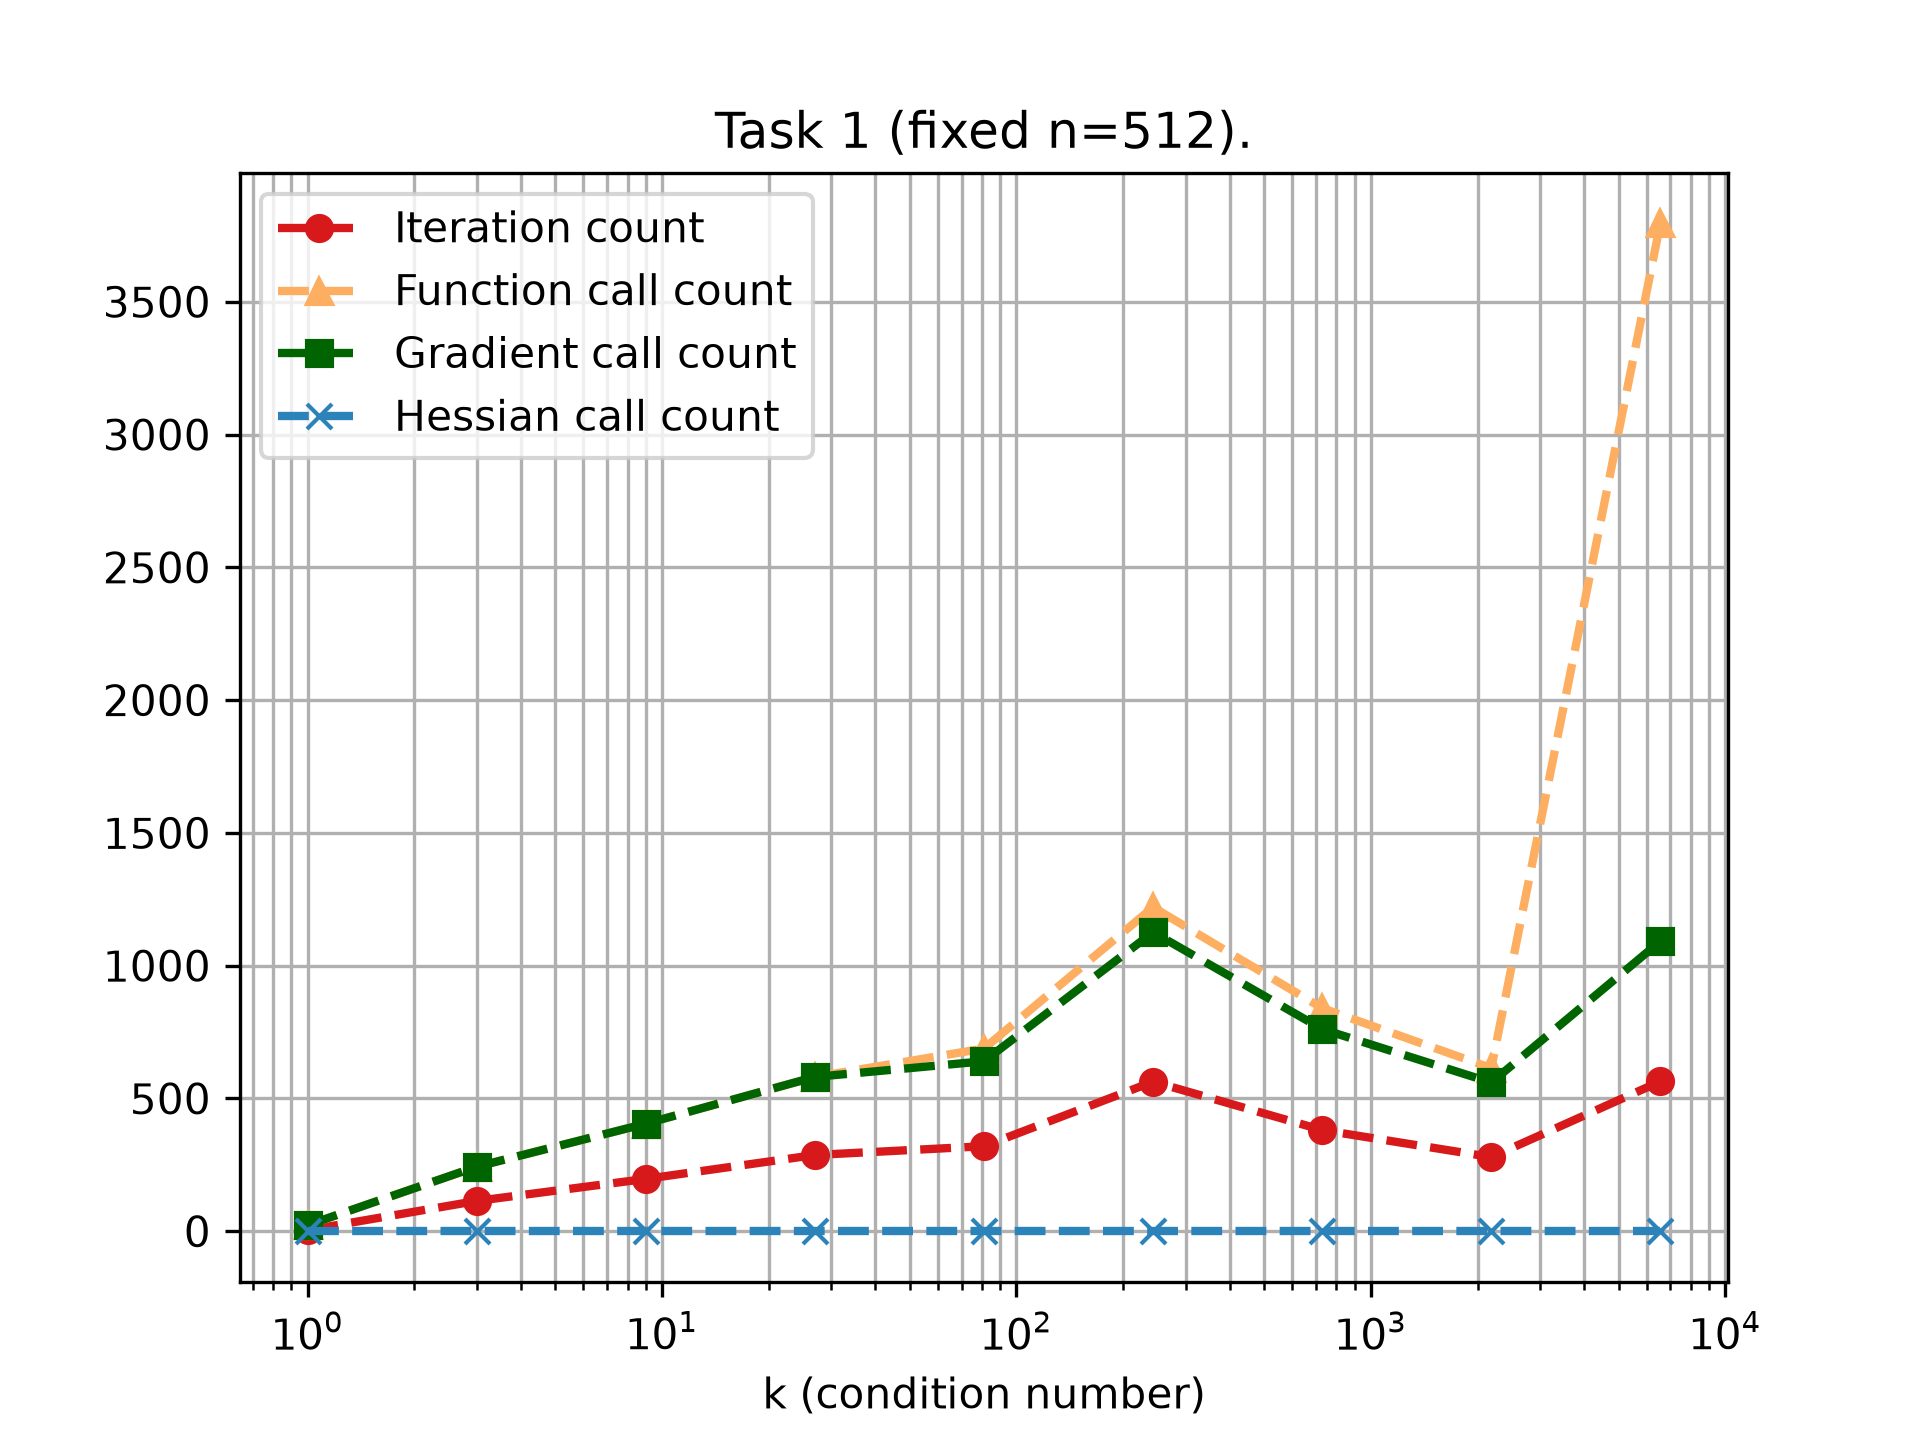
\includegraphics[width=0.5\textwidth]{task1_BFGS_fix_n_512.png}}%
    \caption{Метод BFGS при различных конфигурациях.}
    \end{figure}
    \begin{figure}[H]
    \centering
    \subcaptionbox{Зависимость от $n$ ($k = 3^8$)}{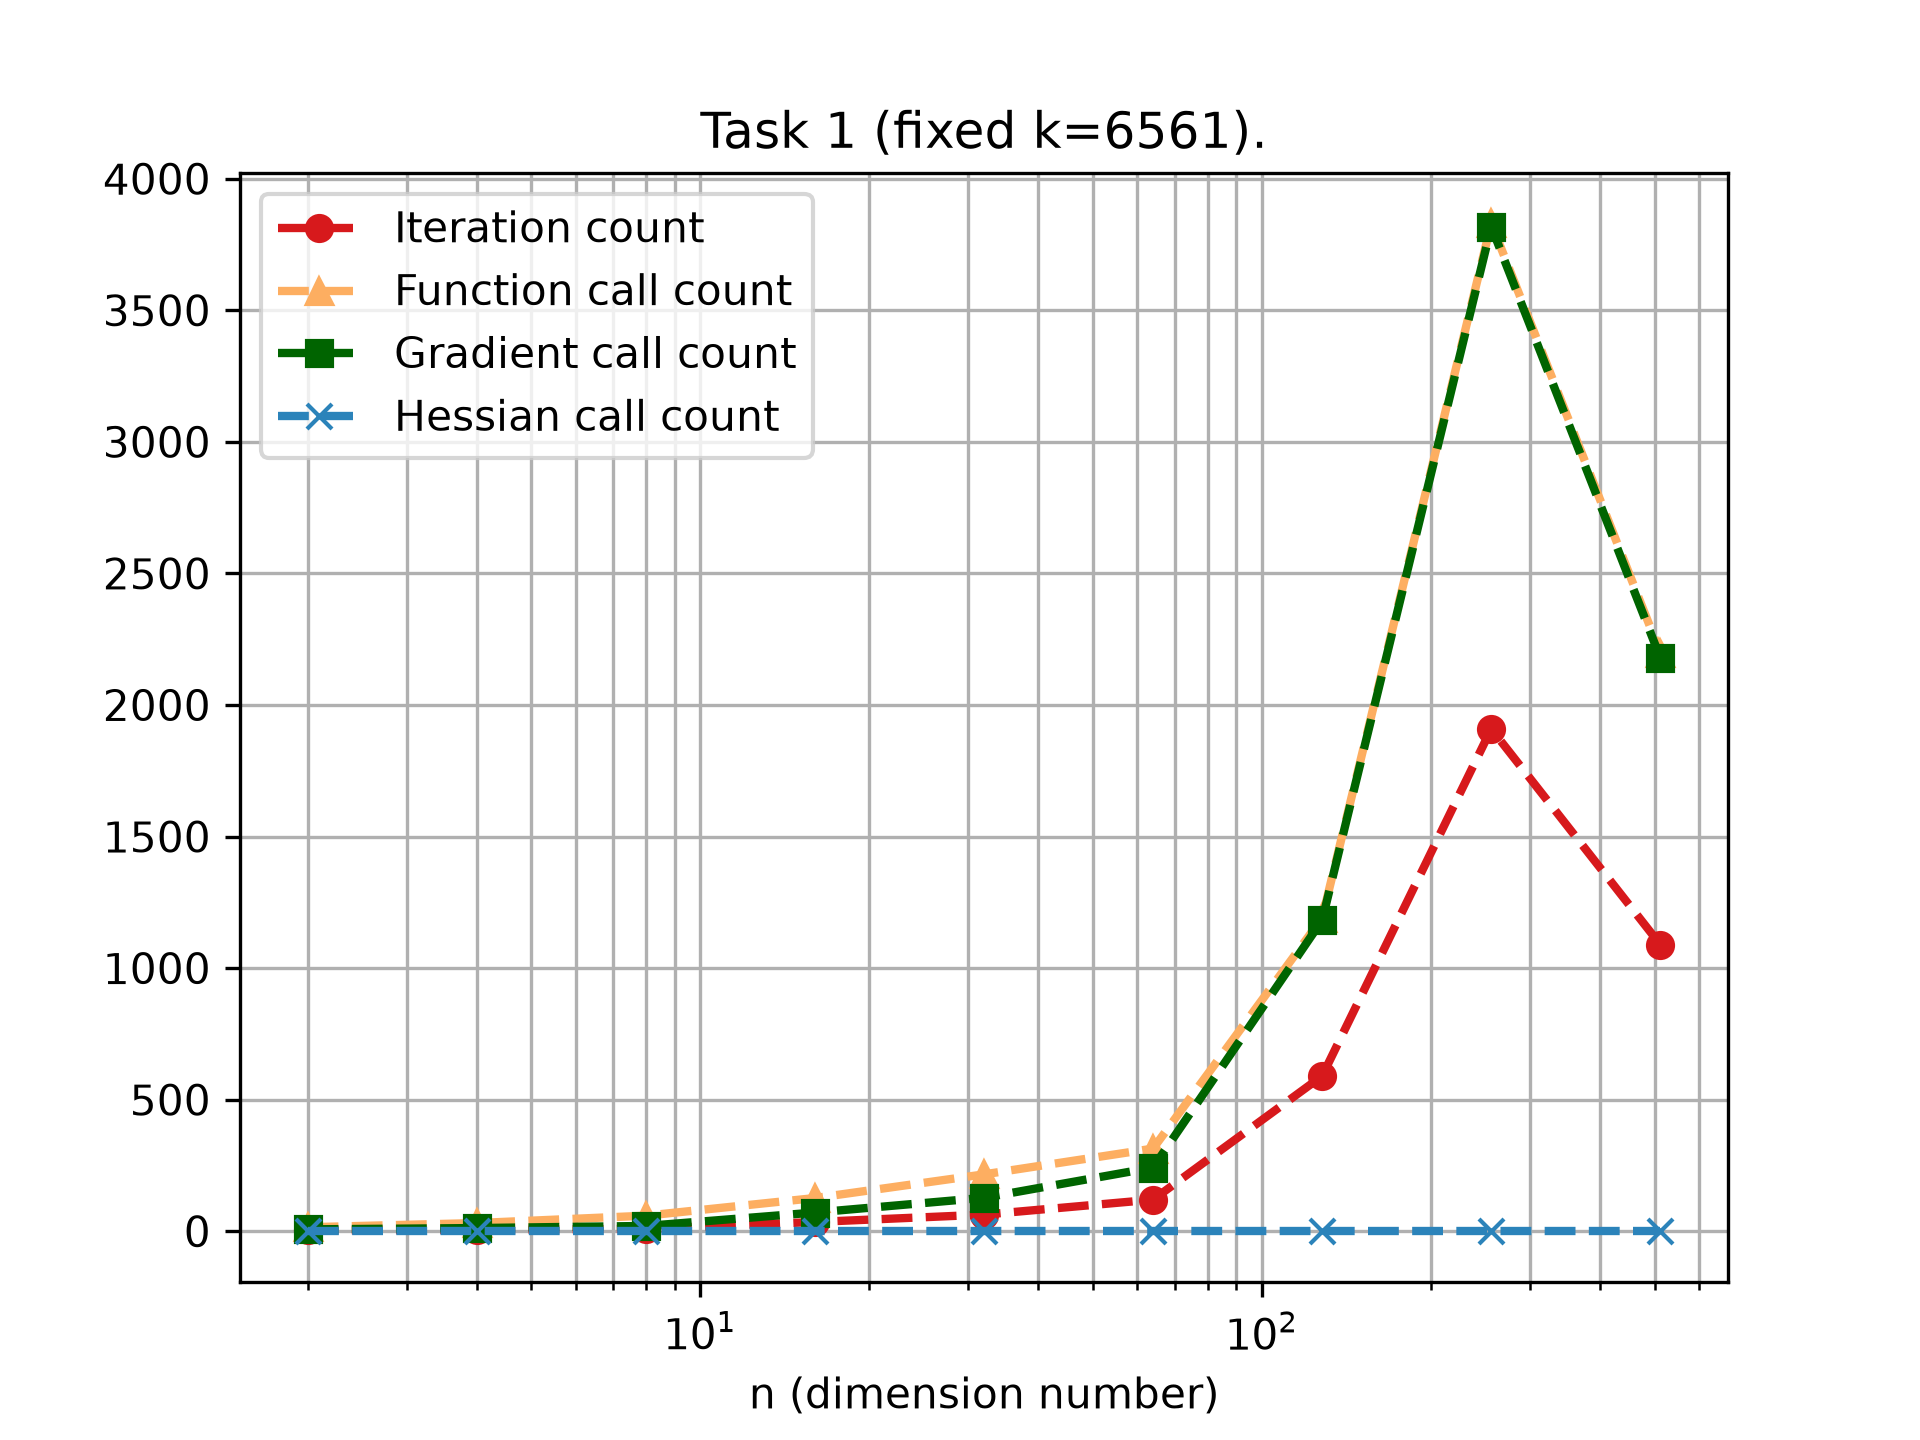
\includegraphics[width=0.5\textwidth]{task1_DFP_fix_k_6561.png}}%
    \subcaptionbox{Зависимость от $k$ ($n = 2^9$)}{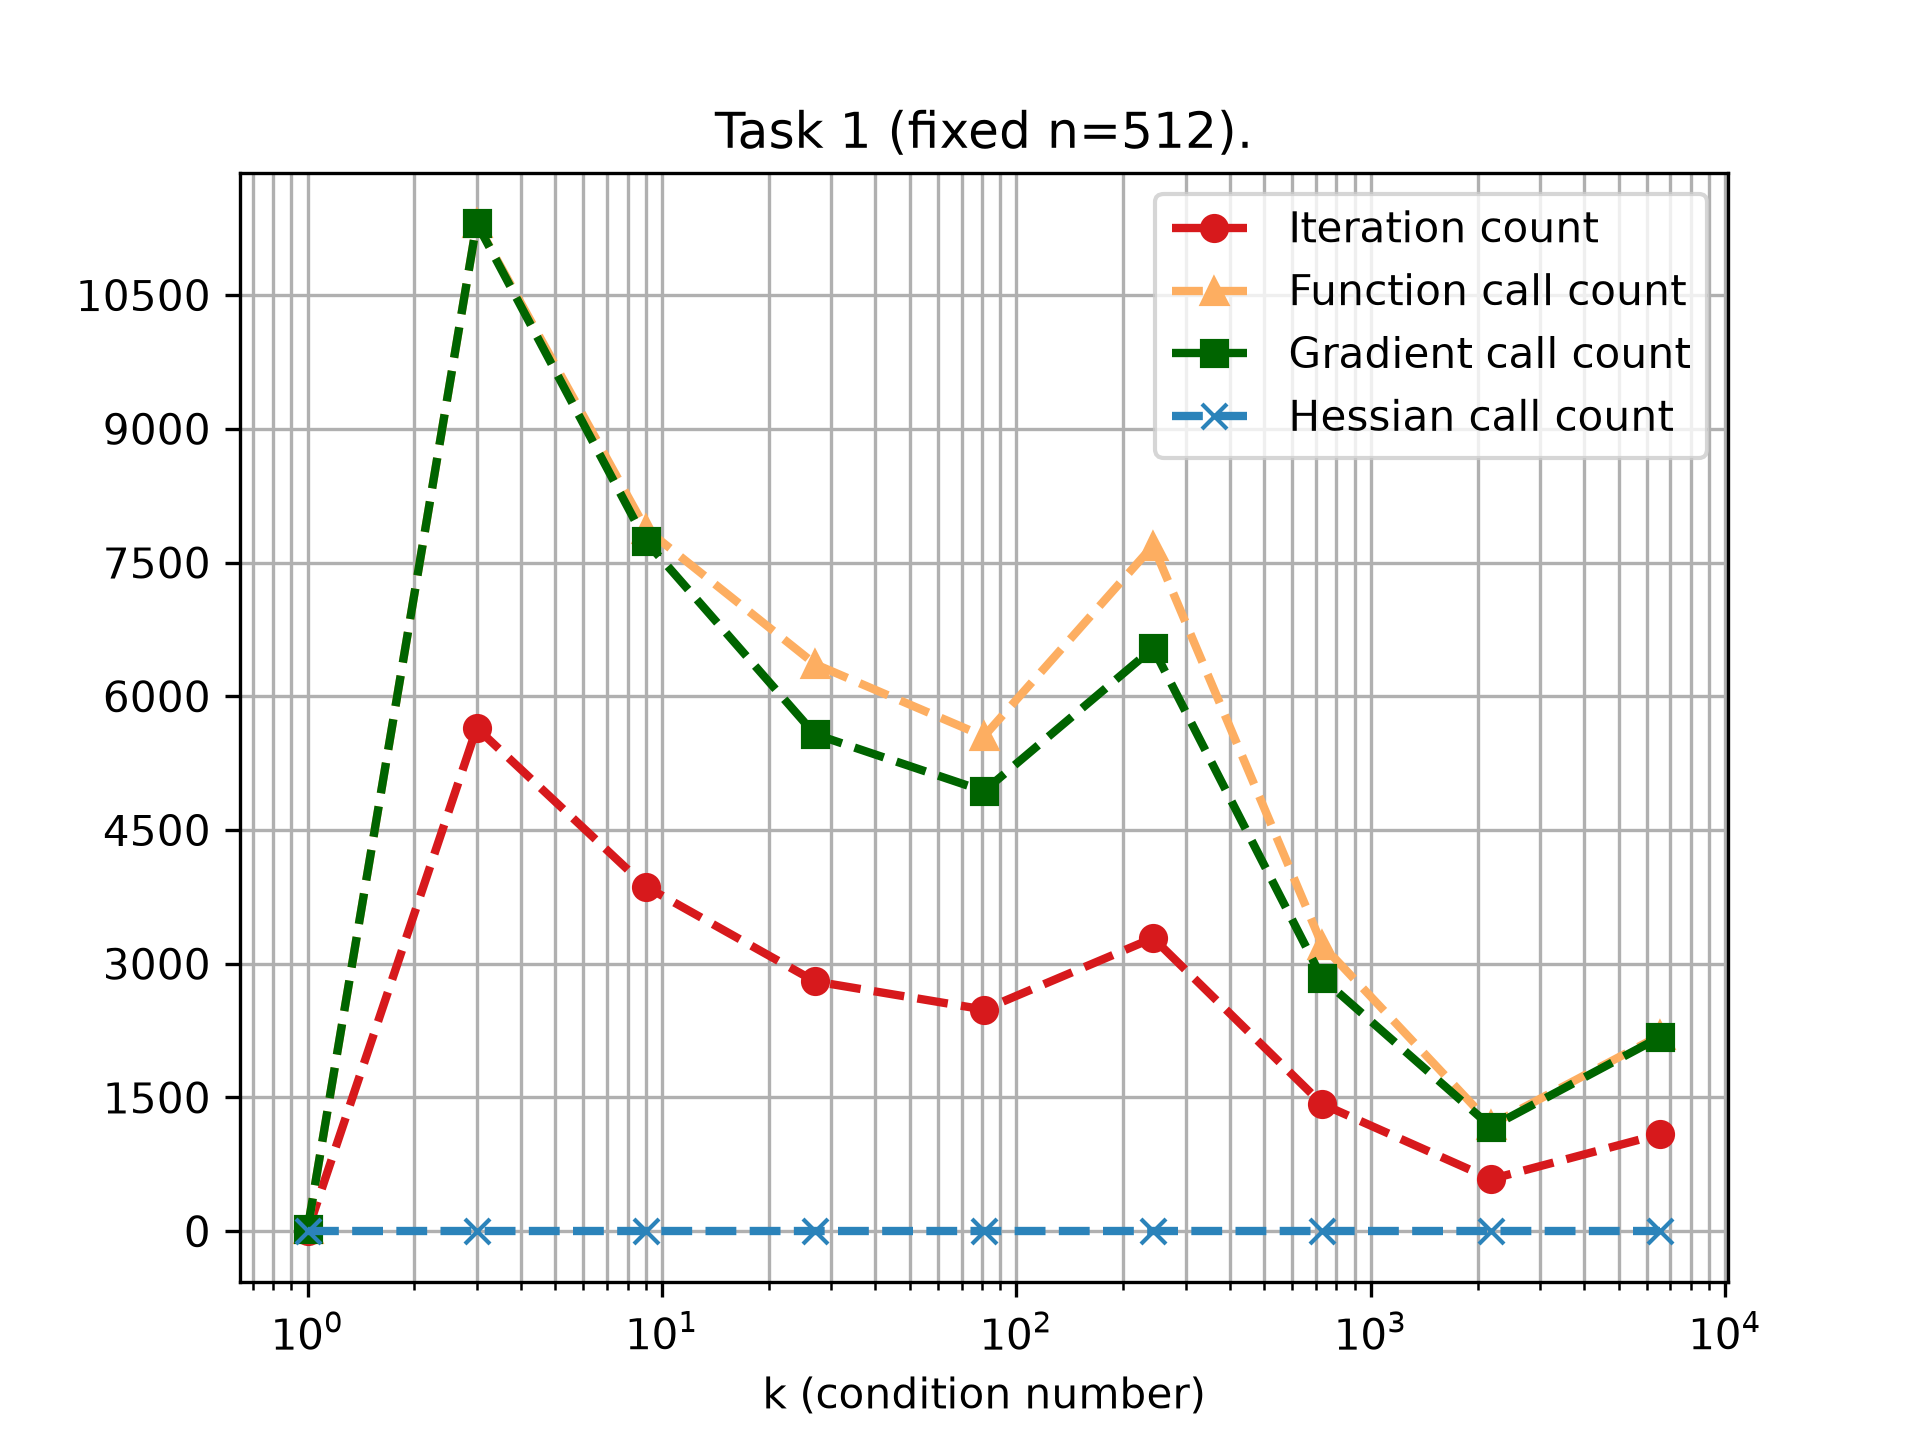
\includegraphics[width=0.5\textwidth]{task1_DFP_fix_n_512.png}}%
    \caption{Метод DFP при различных конфигурациях.}
    \end{figure}
    \item Метод L-BFGS продемонстрировал хаотичный характер возрастания числа итераций при фиксированном $n$ в зависимости от $k$ и весьма конкретный характер возрастания числа итераций при фиксированном $k$ в зависимости от $n$.
    \begin{figure}[H]
    \centering
    \subcaptionbox{Зависимость от $n$ ($k = 3^8$)}{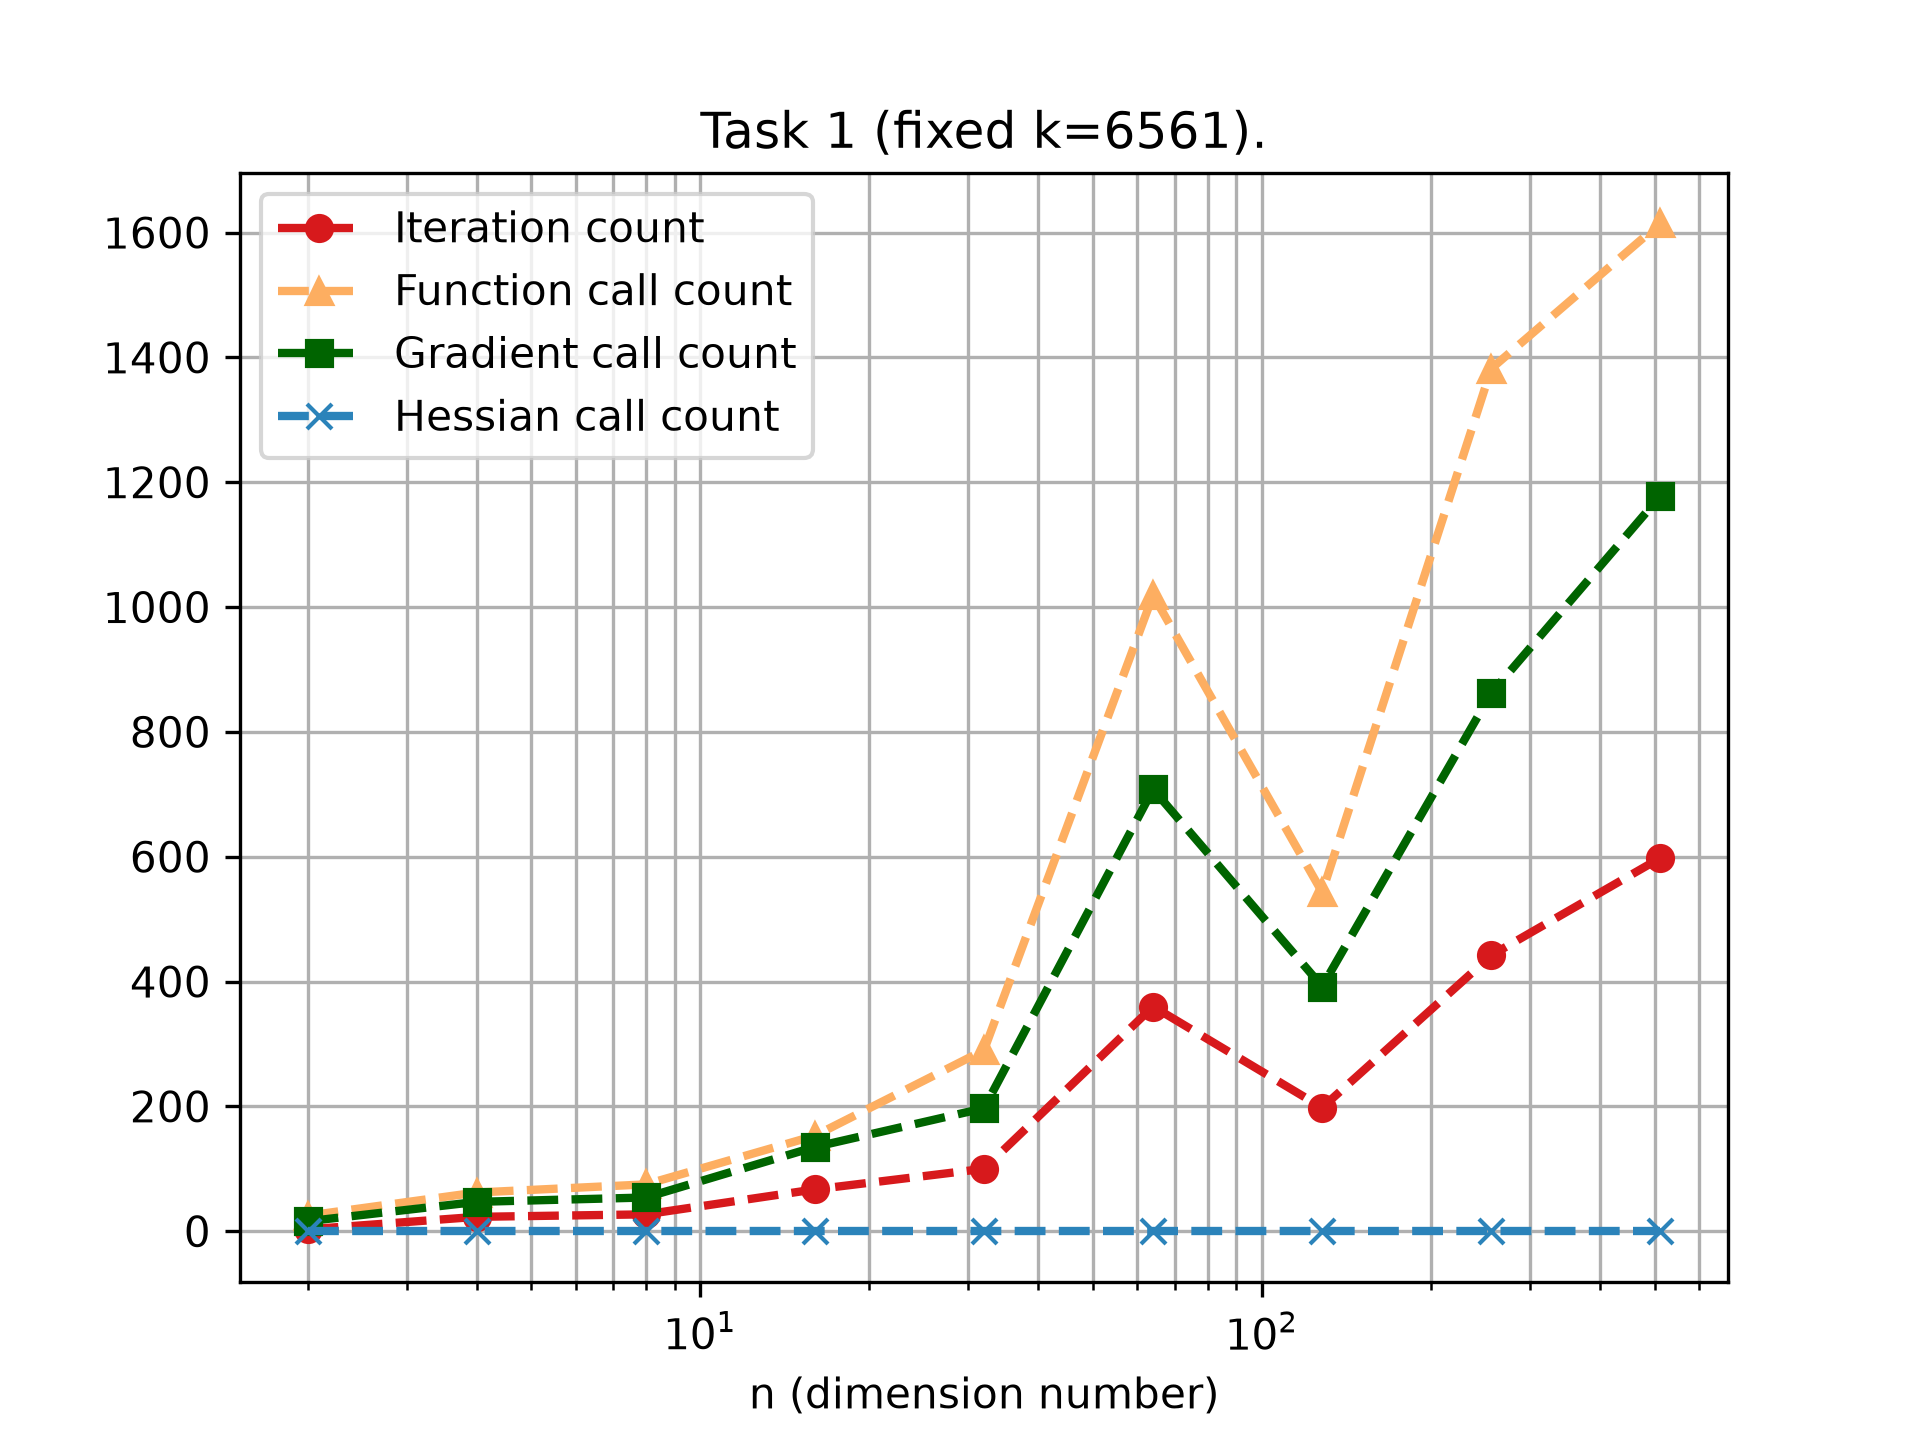
\includegraphics[width=0.5\textwidth]{task1_LBFGS_fix_k_6561.png}}%
    \subcaptionbox{Зависимость от $k$ ($n = 2^9$)}{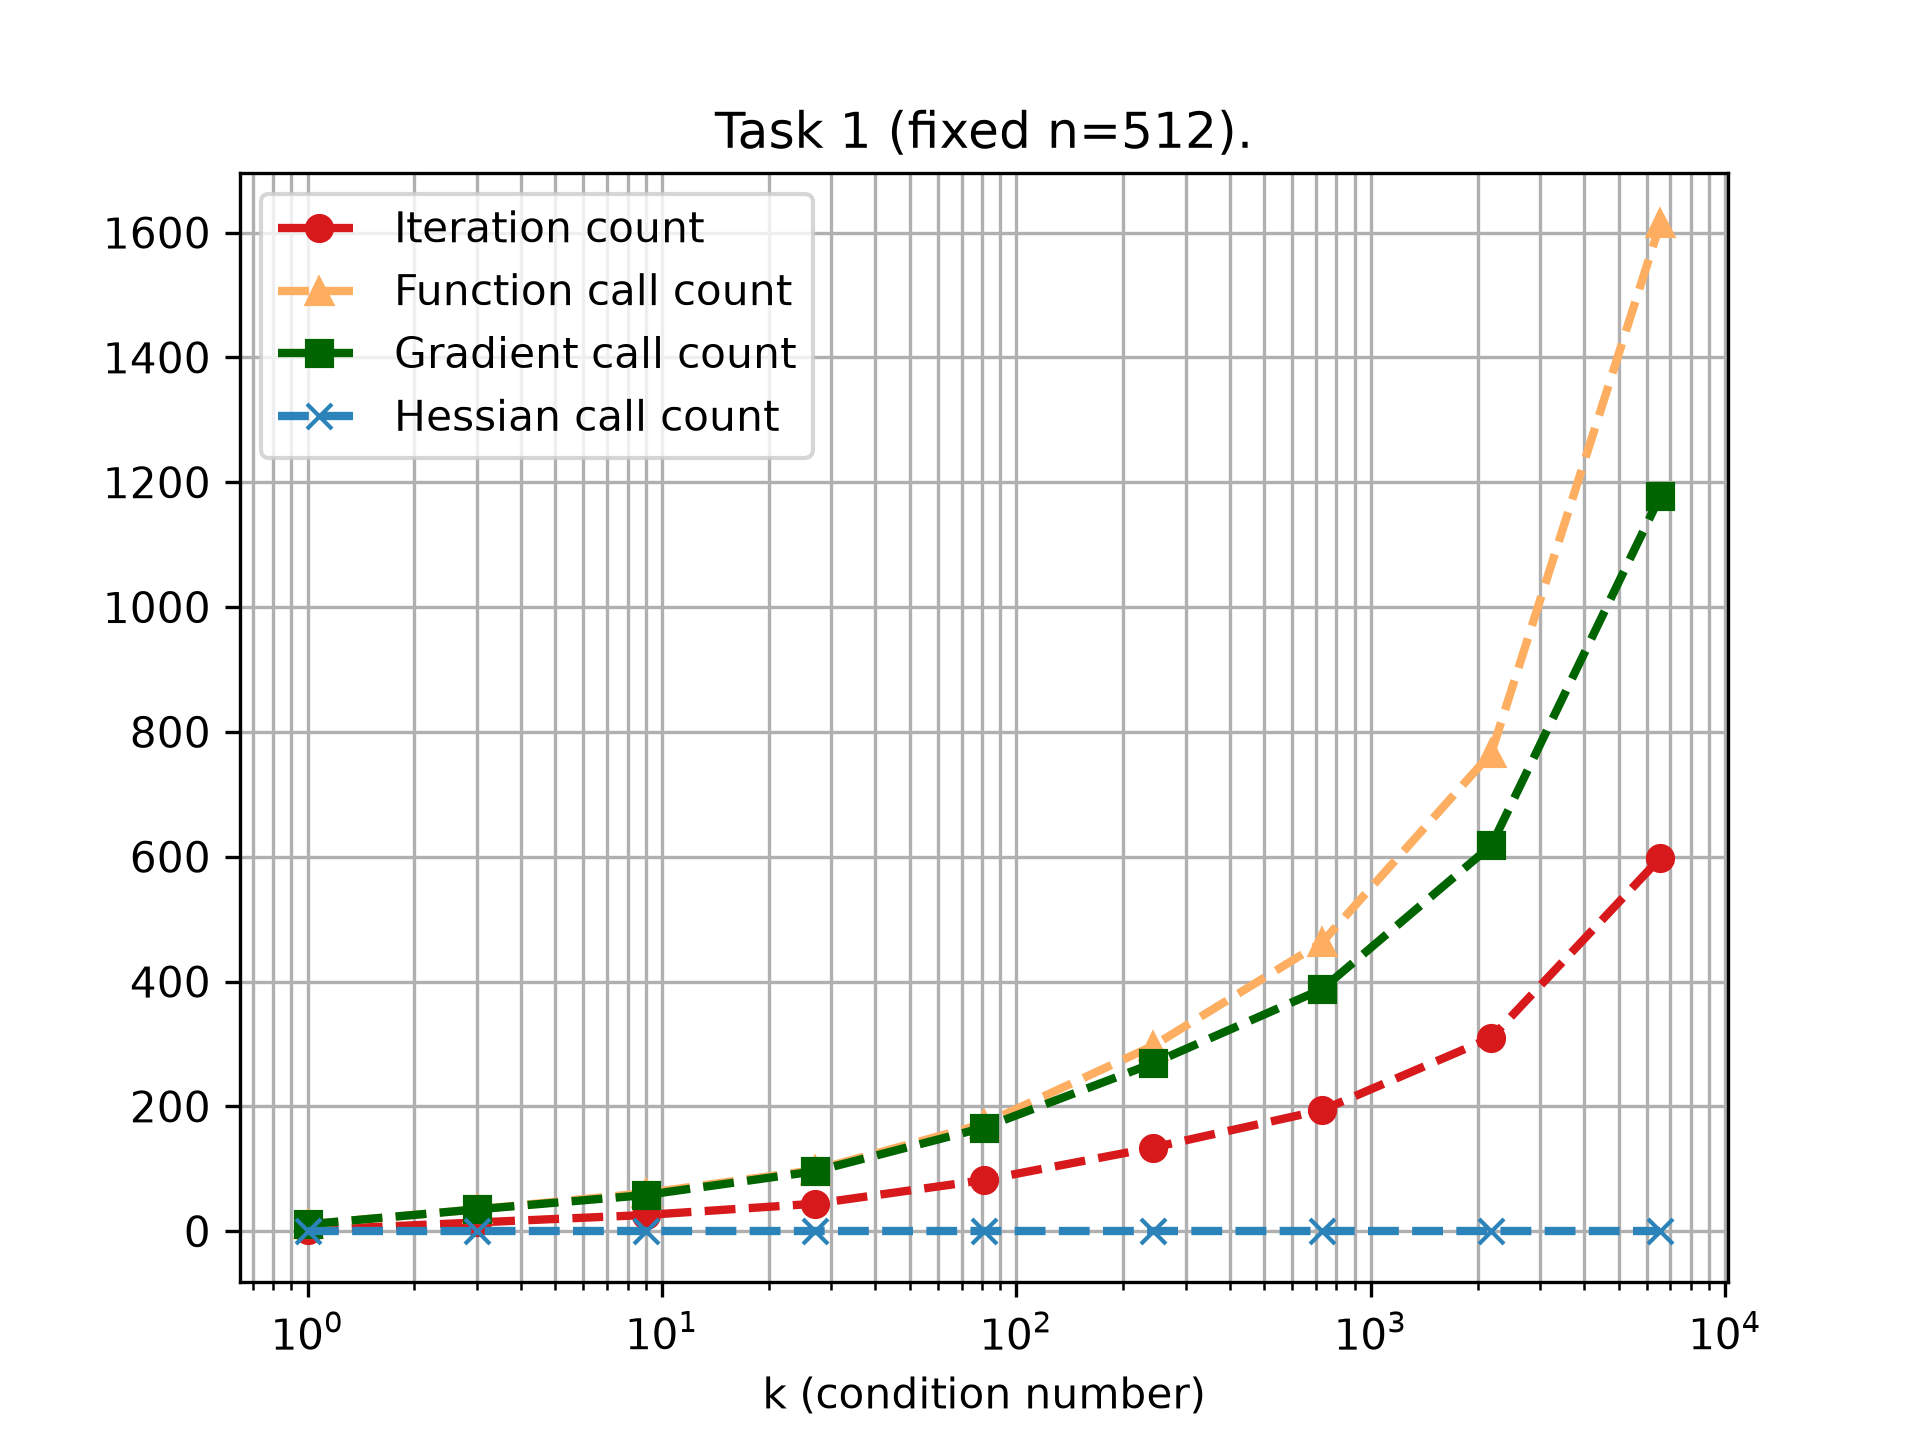
\includegraphics[width=0.5\textwidth]{task1_LBFGS_fix_n_512.png}}%
    \caption{Метод L-BFGS при различных конфигурациях.}
    \end{figure}
    \item Метод NewtonCG (библиотечная реализация) ведёт относительно стабильно. При этом заметна логарифмическая зависимость числа итераций от $k$ при фиксированном $n$. 
    \begin{figure}[H]
    \centering
    \subcaptionbox{Зависимость от $n$ ($k = 3^8$)}{
\includegraphics[width=0.5\textwidth]{task1_NewtonCG_fix_k_6561.png}}%
    \subcaptionbox{Зависимость от $k$ ($n = 2^9$)}{
\includegraphics[width=0.5\textwidth]{task1_NewtonCG_fix_n_512.png}}%
    \caption{Метод NewtonCG при различных конфигурациях.}
    \end{figure}
\end{itemize}

Таким образом, методы Ньютона с использованием разложения Холецкого, метод Ньютона с выбором шага и Powell's Dog Leg продемонстрировали более оптимальные и стабильные результаты работы по сравнению с библиотечной реализацией NewtonCG. В то же время, NewtonCG показал себя лучшим методом по сравнению с методами сопряжённых коэффициентов, нелинейных сопряжённых коэффициентов и квазиньютоновскими методами.

Ниже приведена иллюстрация работы всех собственных реализаций на примере двумерной квадратичной функции с $k=10$. Запуски проводились из 5 точек с разными расстояниями от центра.

\begin{figure}[H]
\centering
\subcaptionbox{Сопр. градиенты}{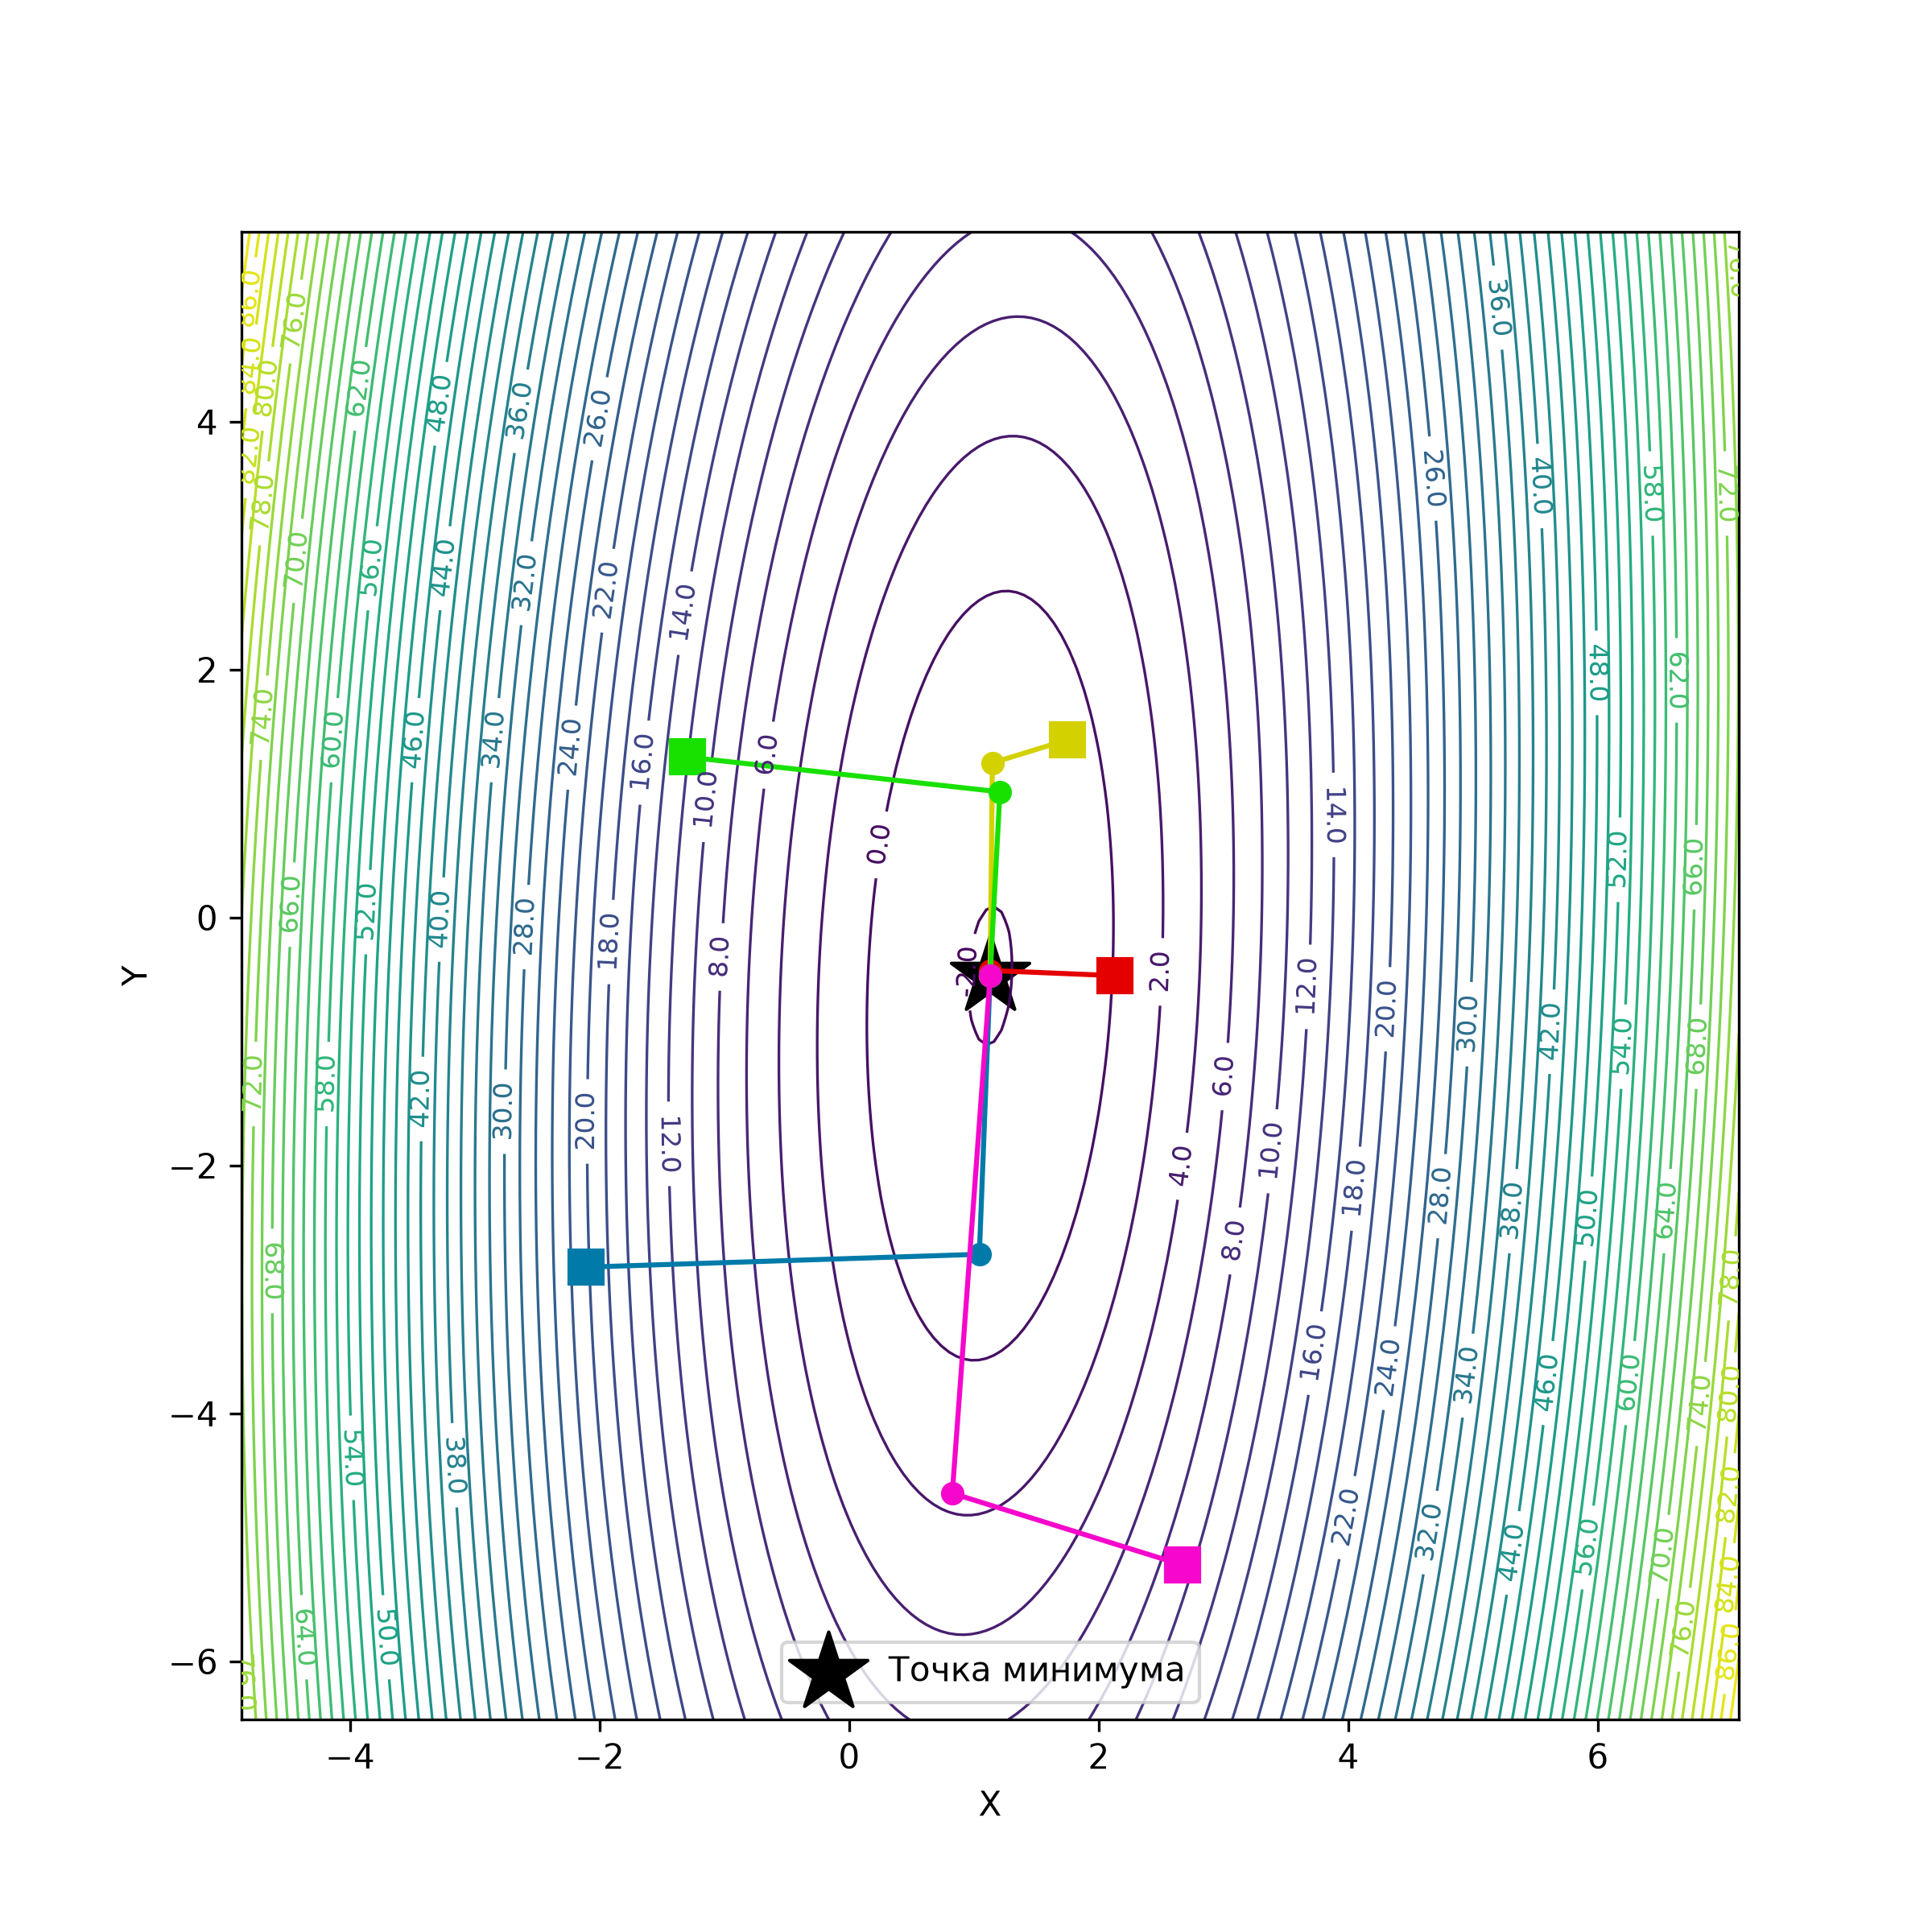
\includegraphics[width=0.3\textwidth]{task2_LinearConjugateGradient_plot.png}}%
\hfill % <-- Seperation
\subcaptionbox{Флетчер-Ривс}{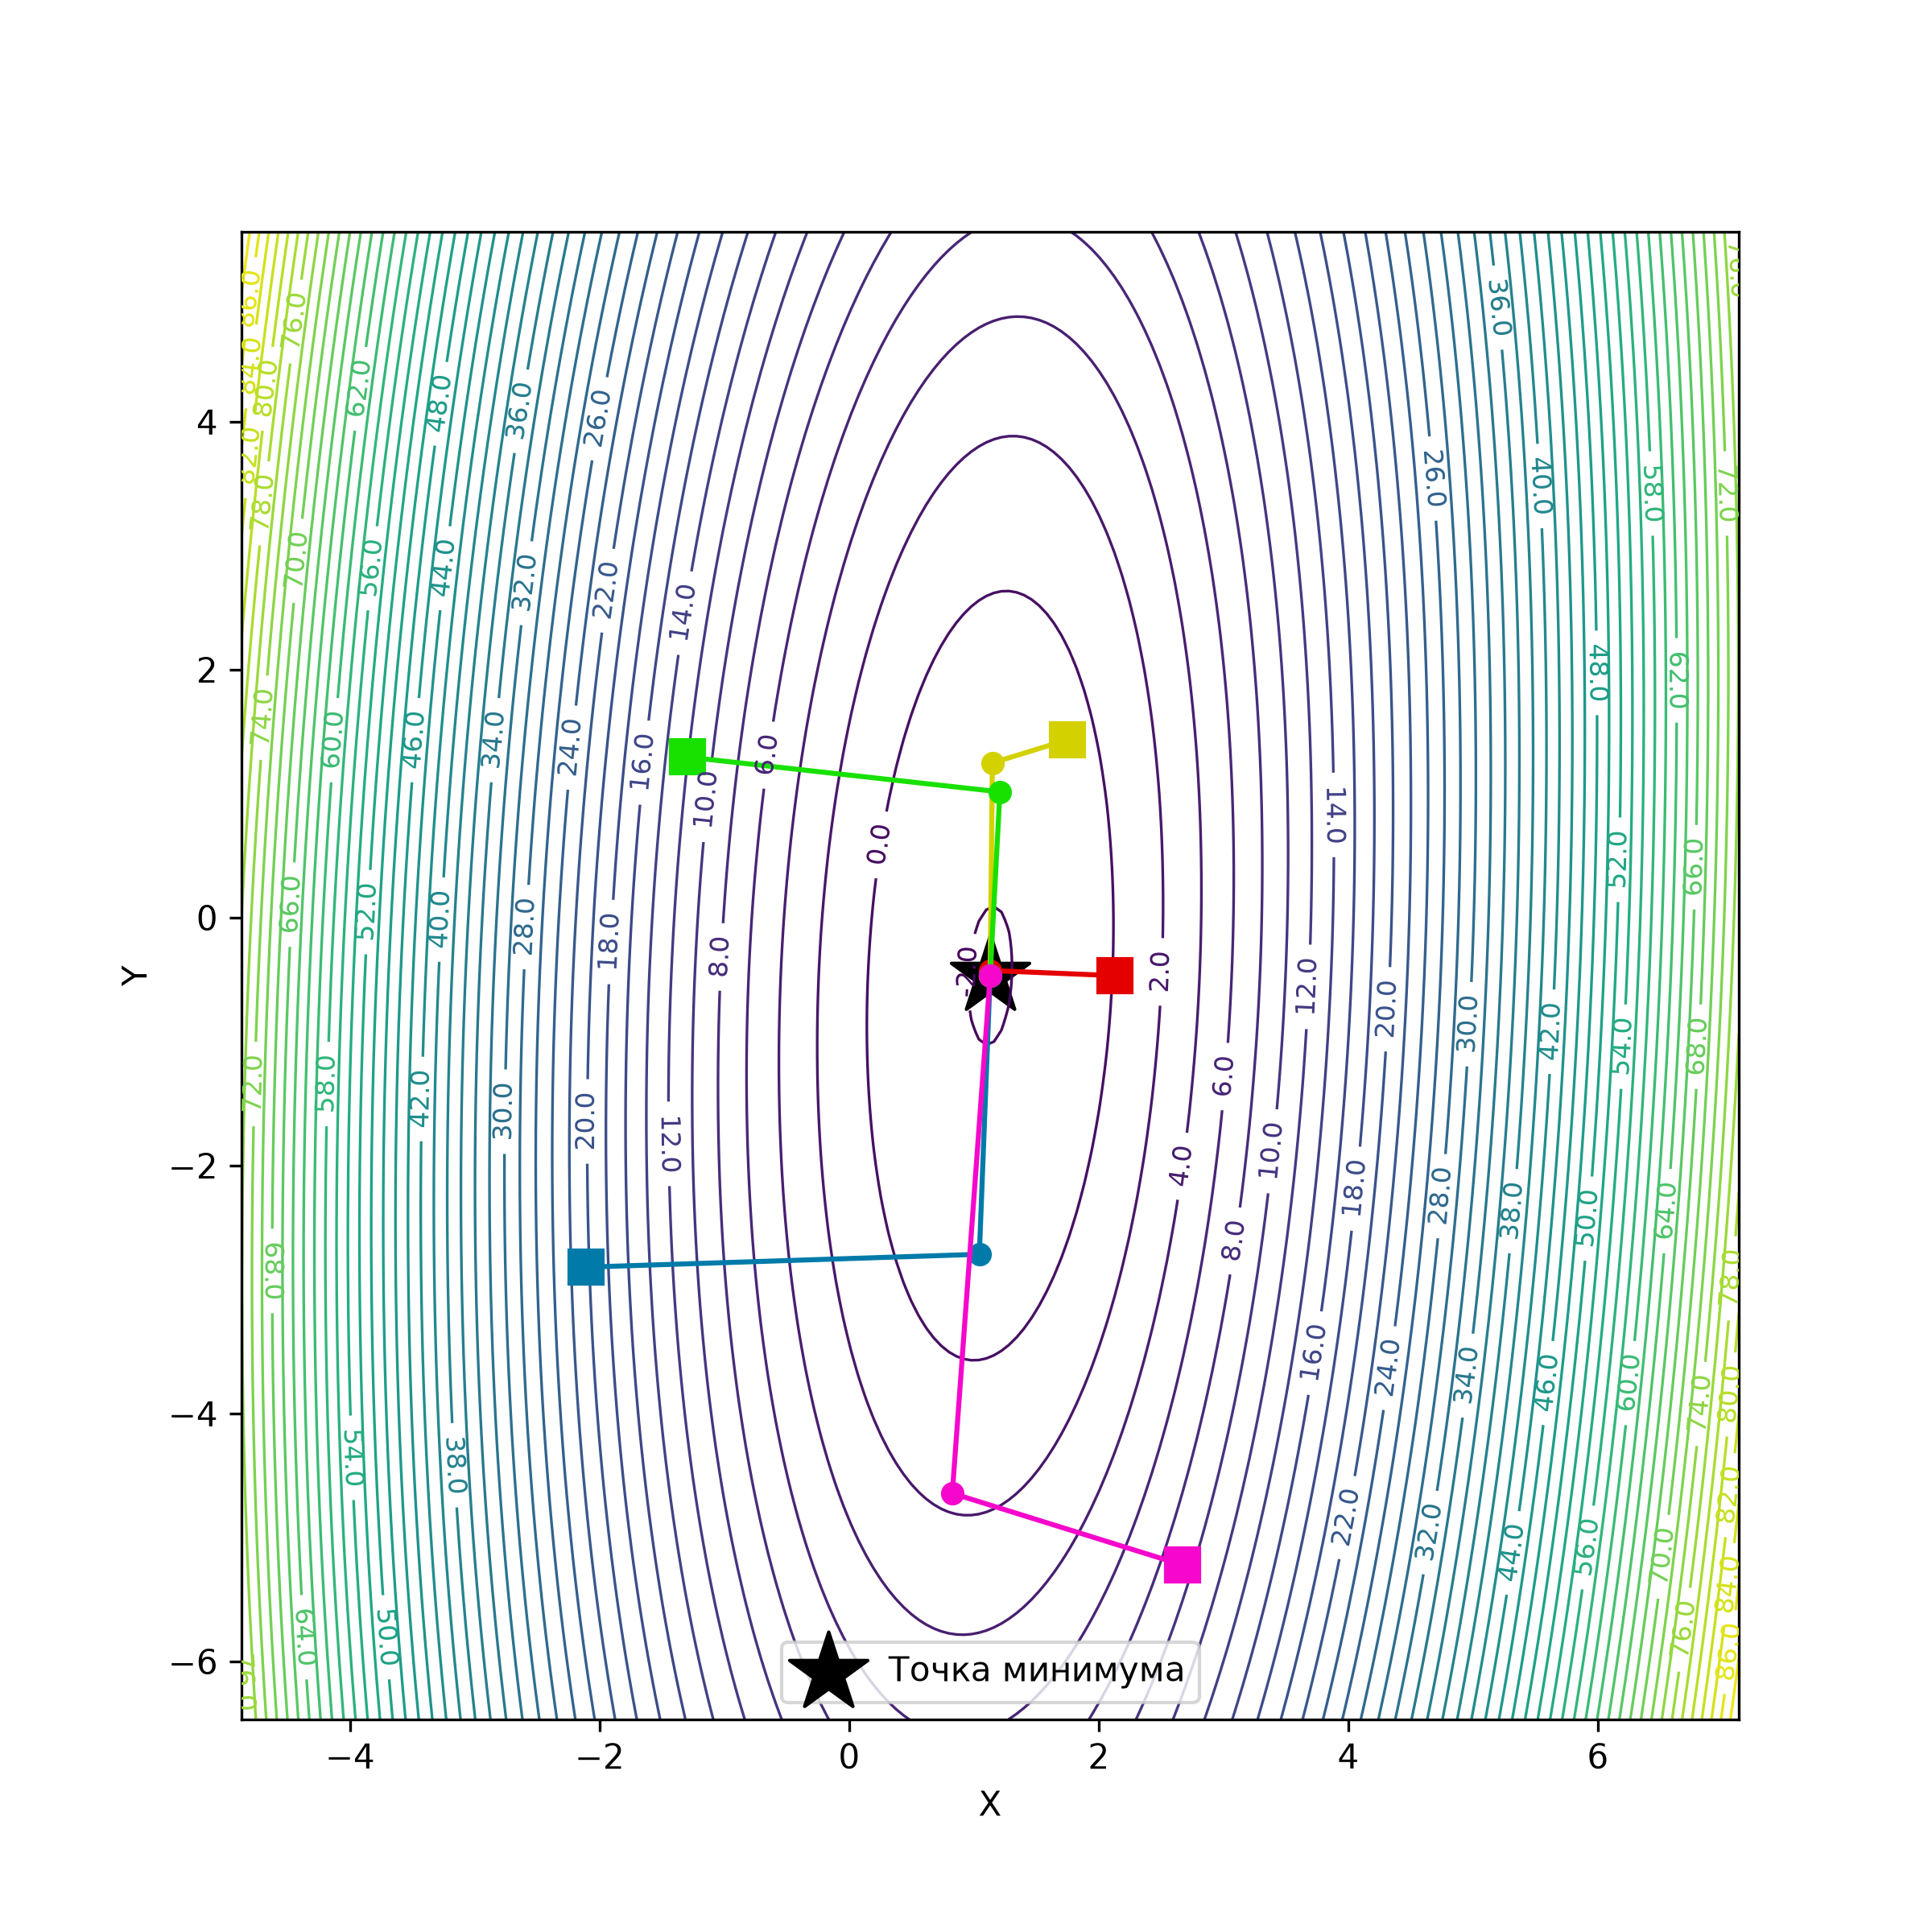
\includegraphics[width=0.3\textwidth]{task2_FletcherReeves_plot.png}}%
\hfill % <-- Seperation
\subcaptionbox{Полак-Рибьер}{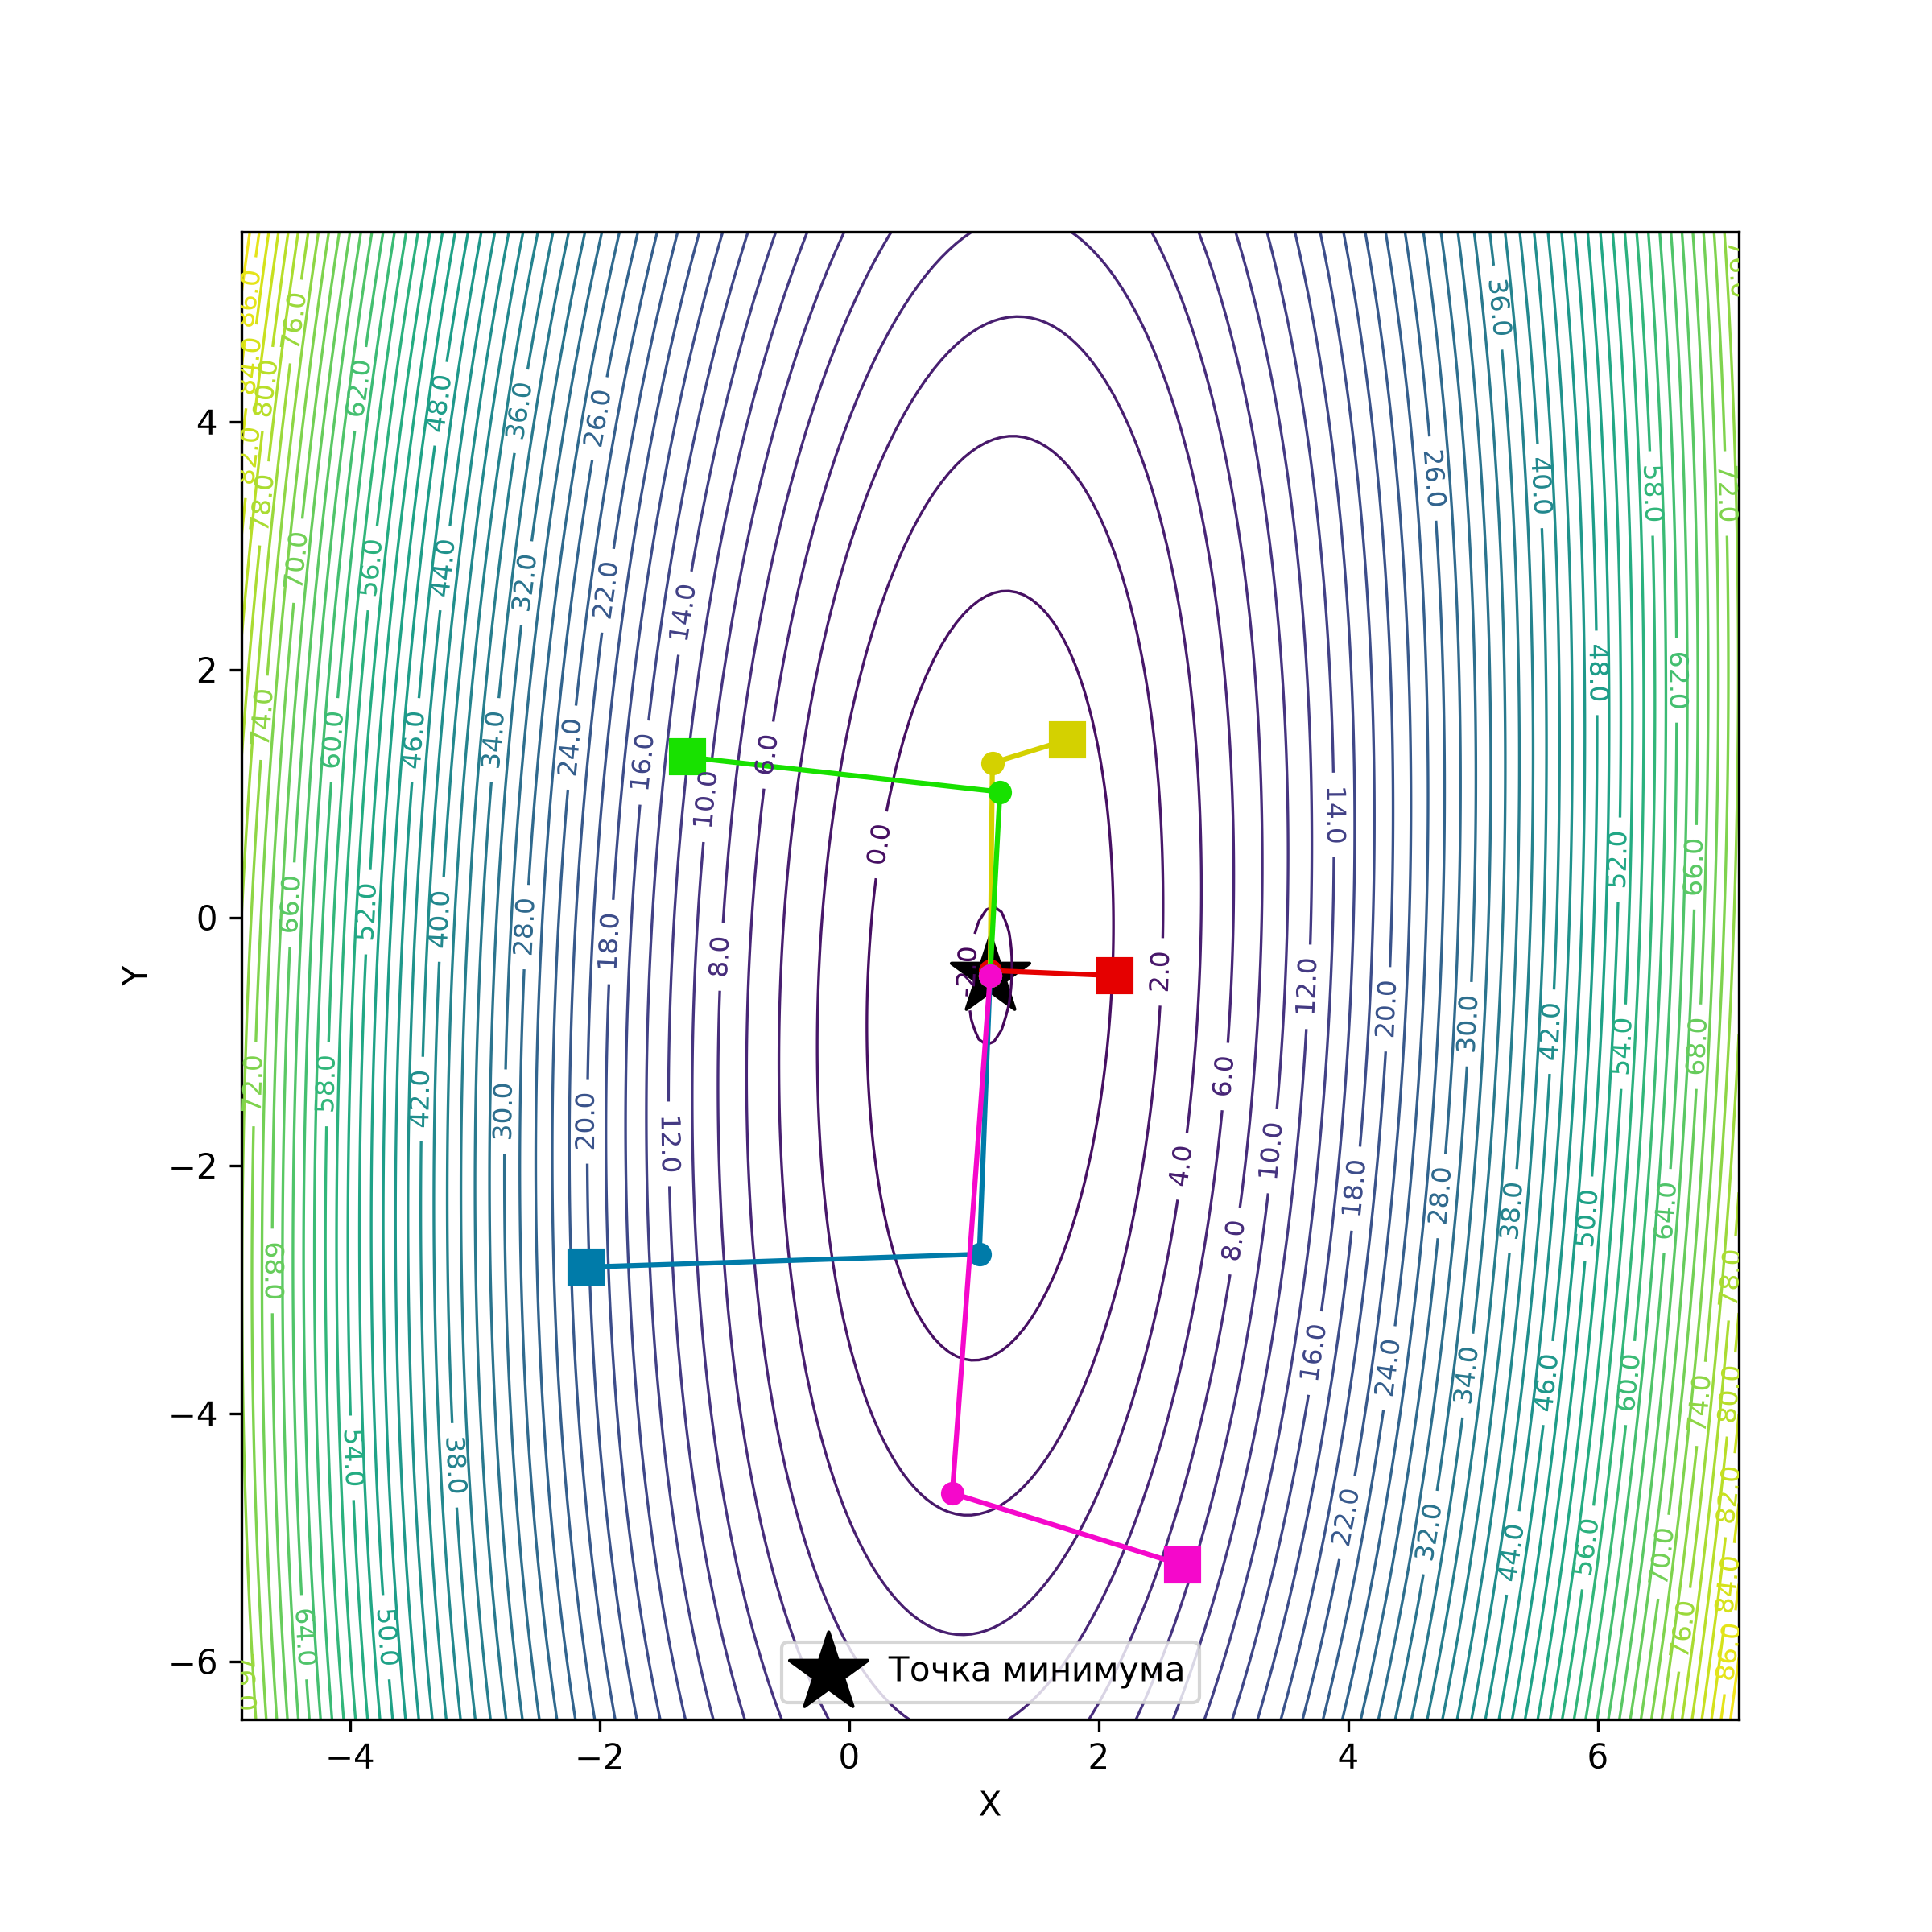
\includegraphics[width=0.3\textwidth]{task2_PolakRibiere_plot.png}}%
\\ % <-- Line break
\centering
\subcaptionbox{Разл. Холецкого}{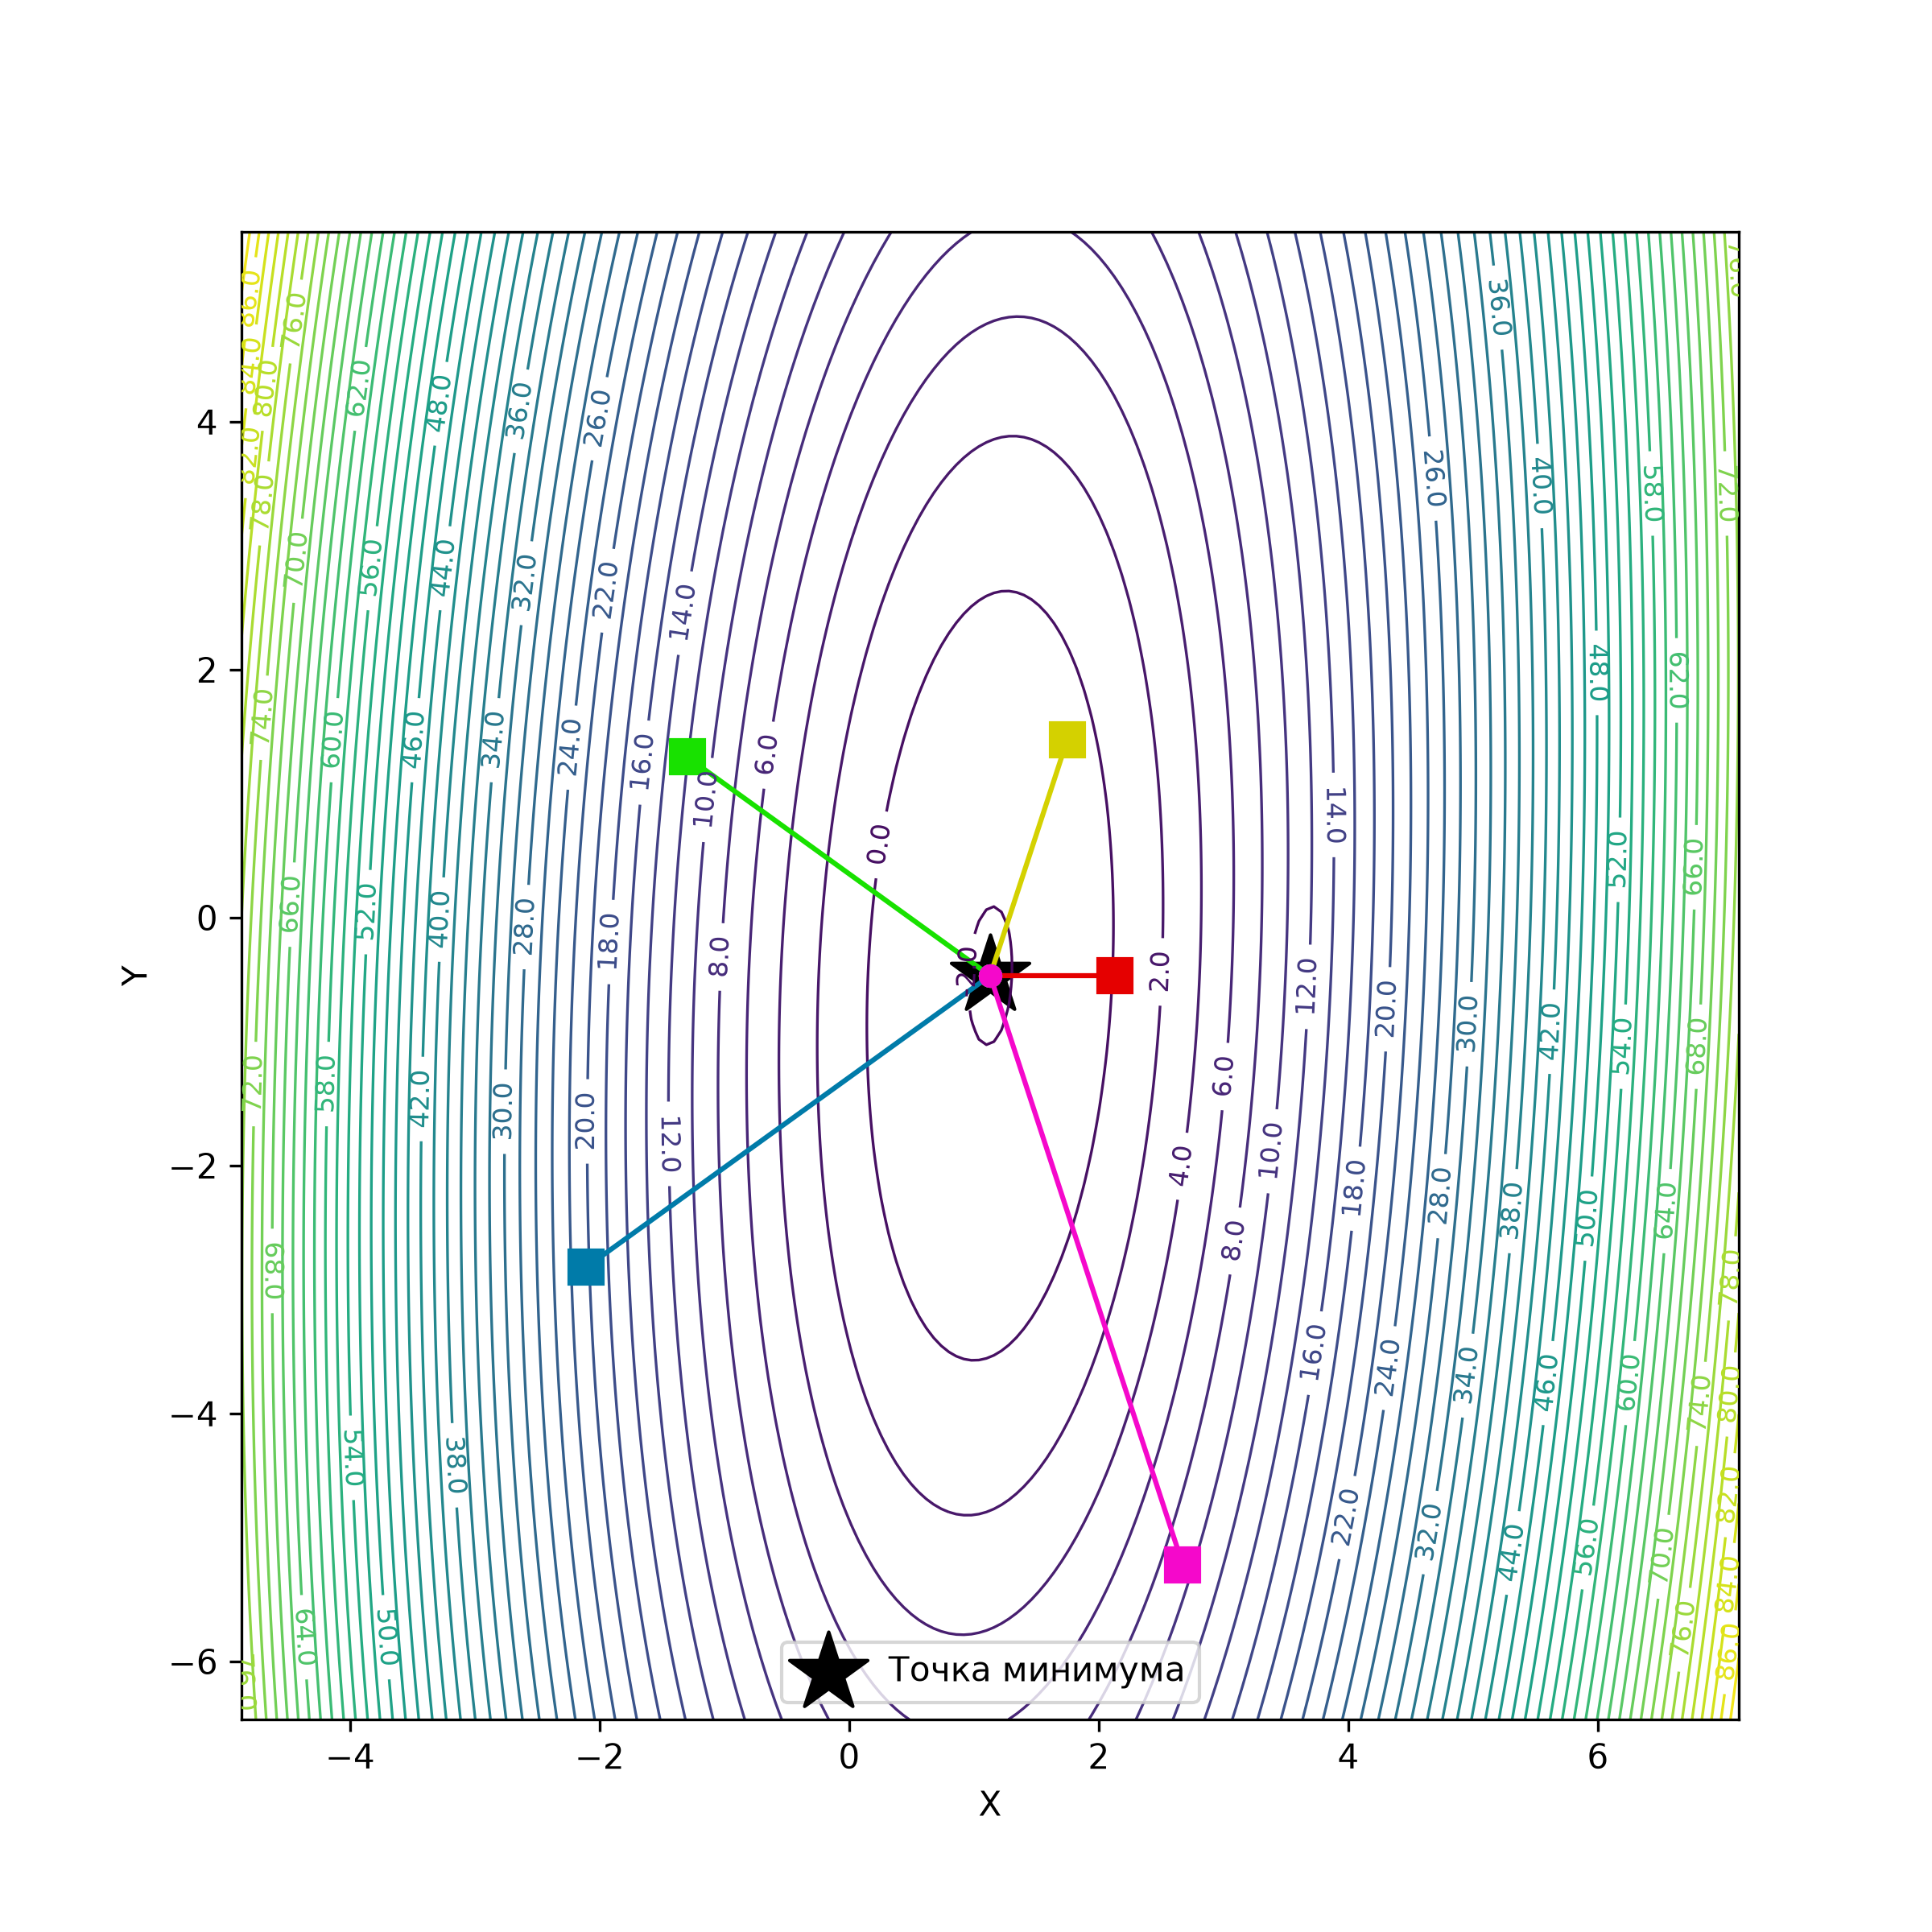
\includegraphics[width=0.3\textwidth]{task2_NewtonCholesky_plot.png}}%
\hfill % <-- Seperation
\subcaptionbox{Выбор направления}{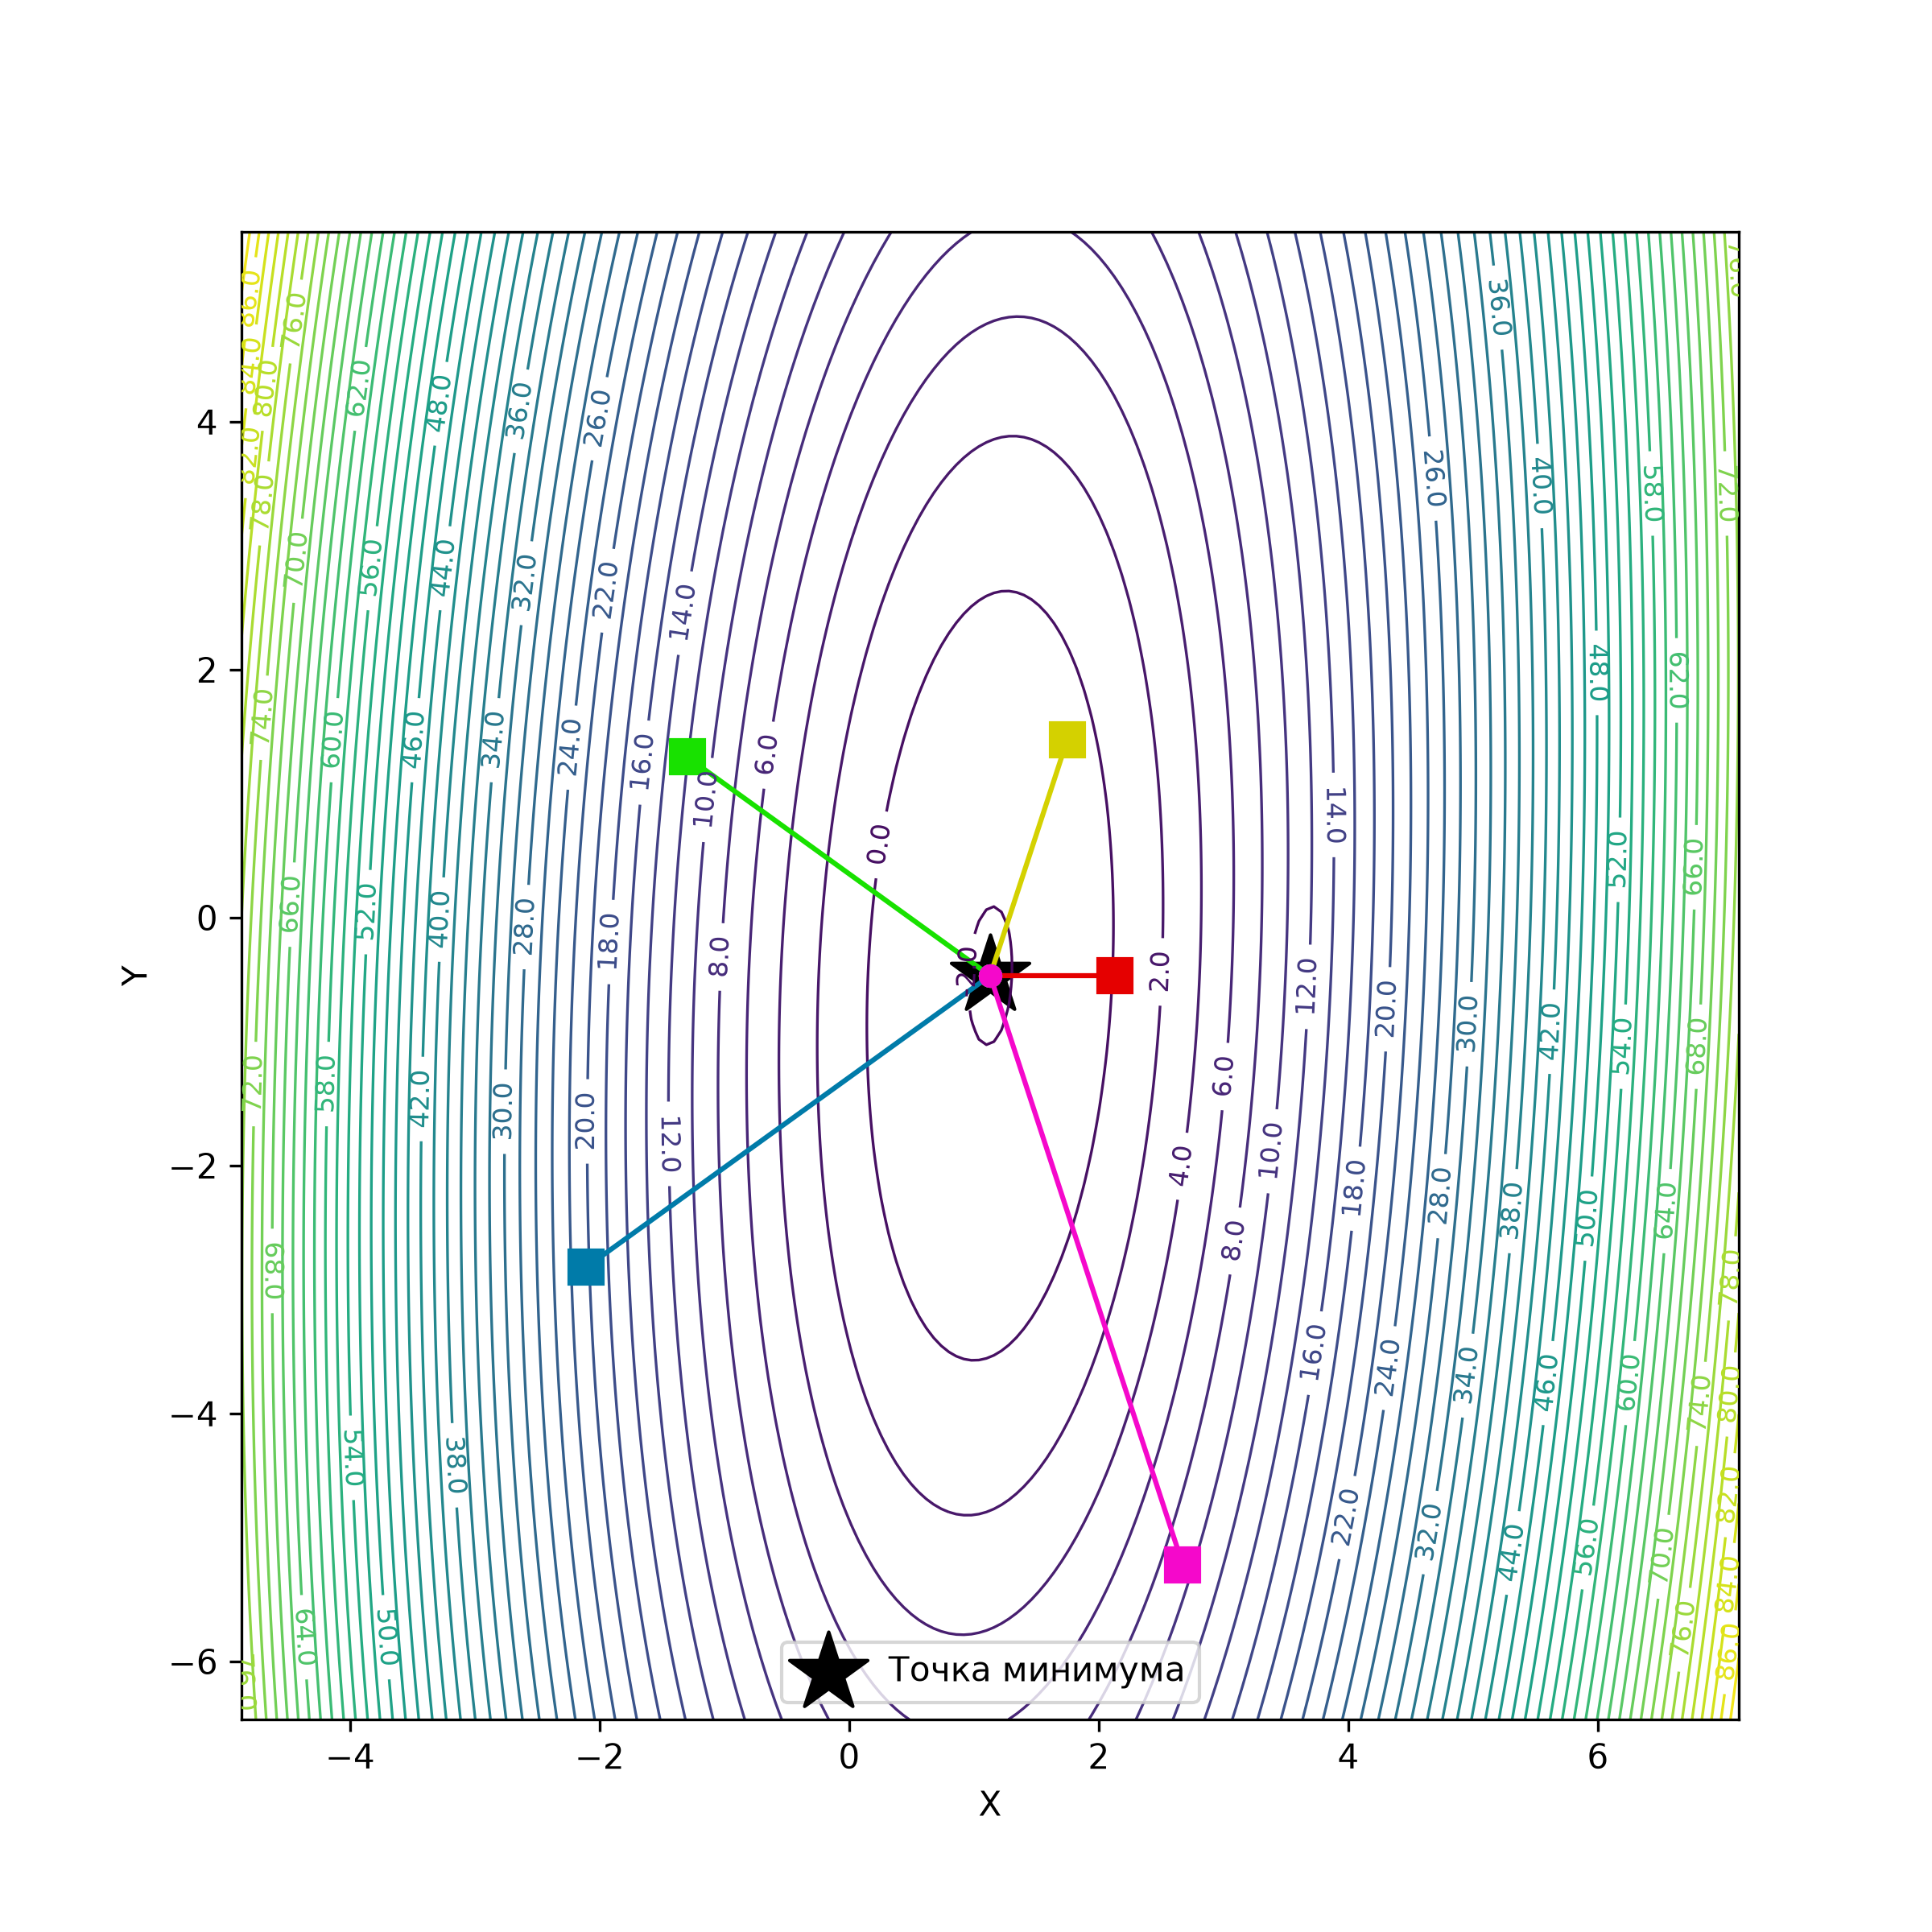
\includegraphics[width=0.3\textwidth]{task2_NewtonDirection_plot.png}}%
\hfill % <-- Seperation
\subcaptionbox{Powell's Dog Leg}{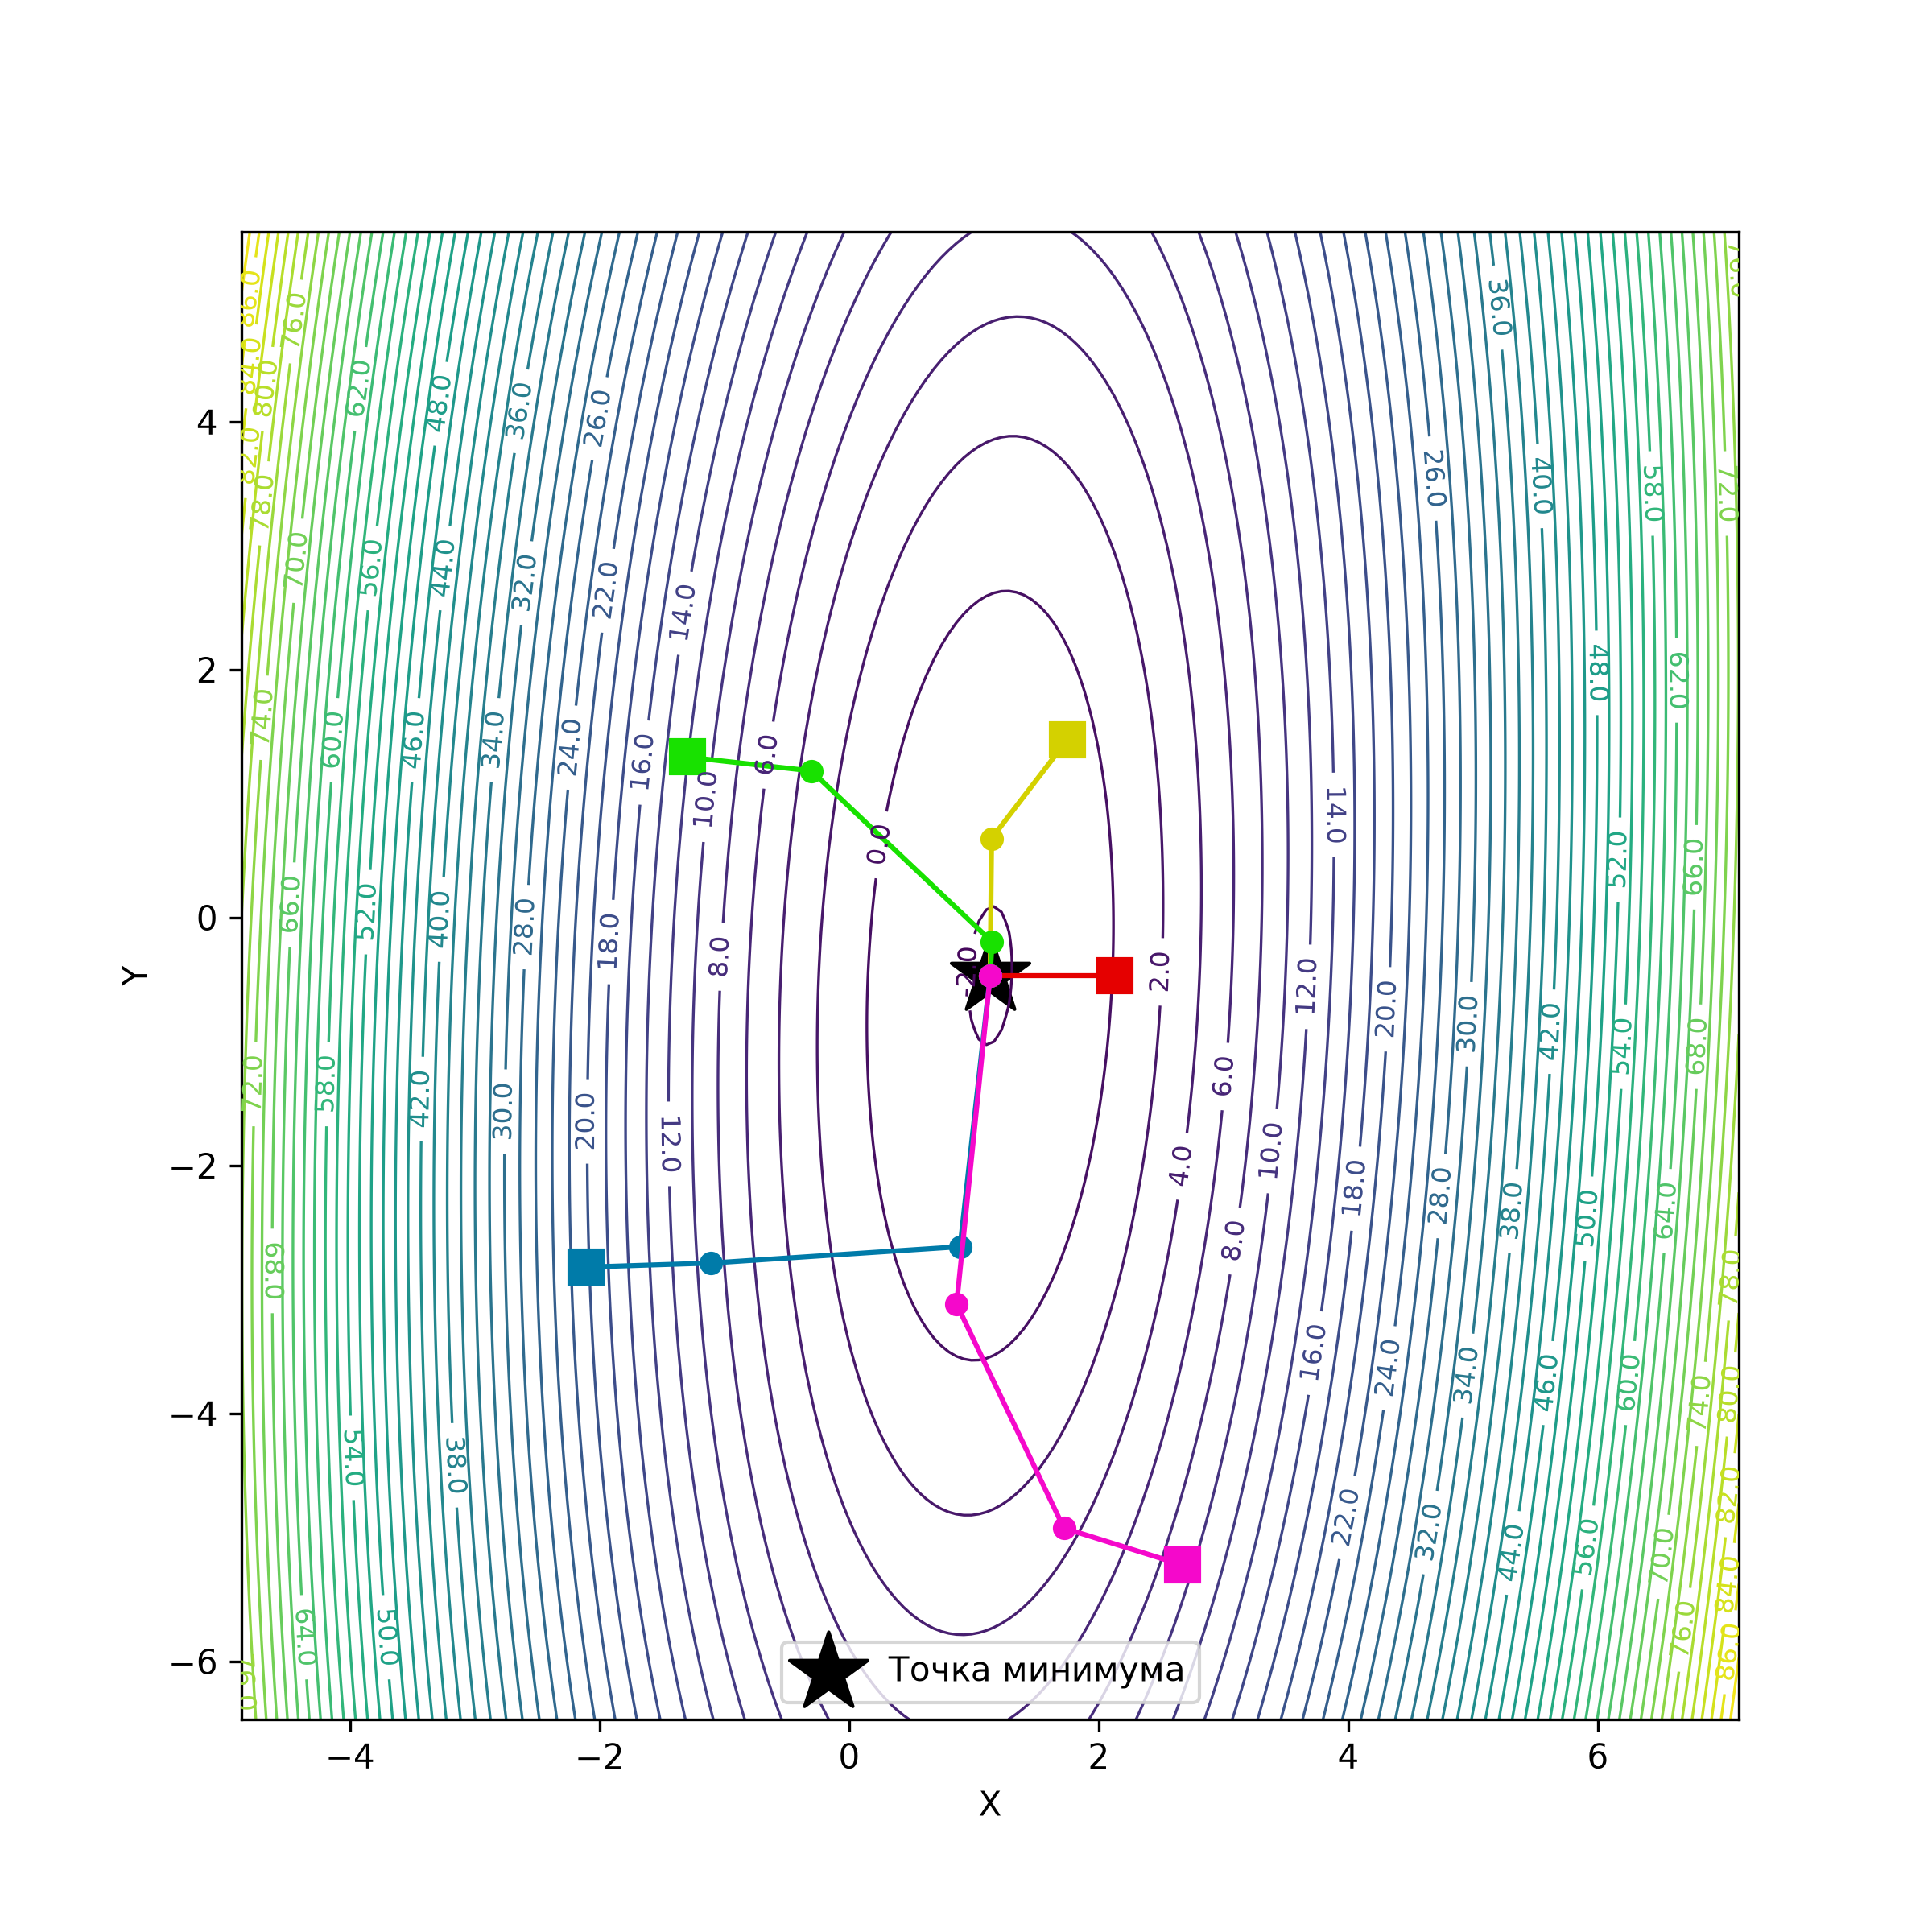
\includegraphics[width=0.3\textwidth]{task2_PowellsDogLeg_plot.png}}%
\\ % <-- Line break
\centering
\subcaptionbox{DFP}{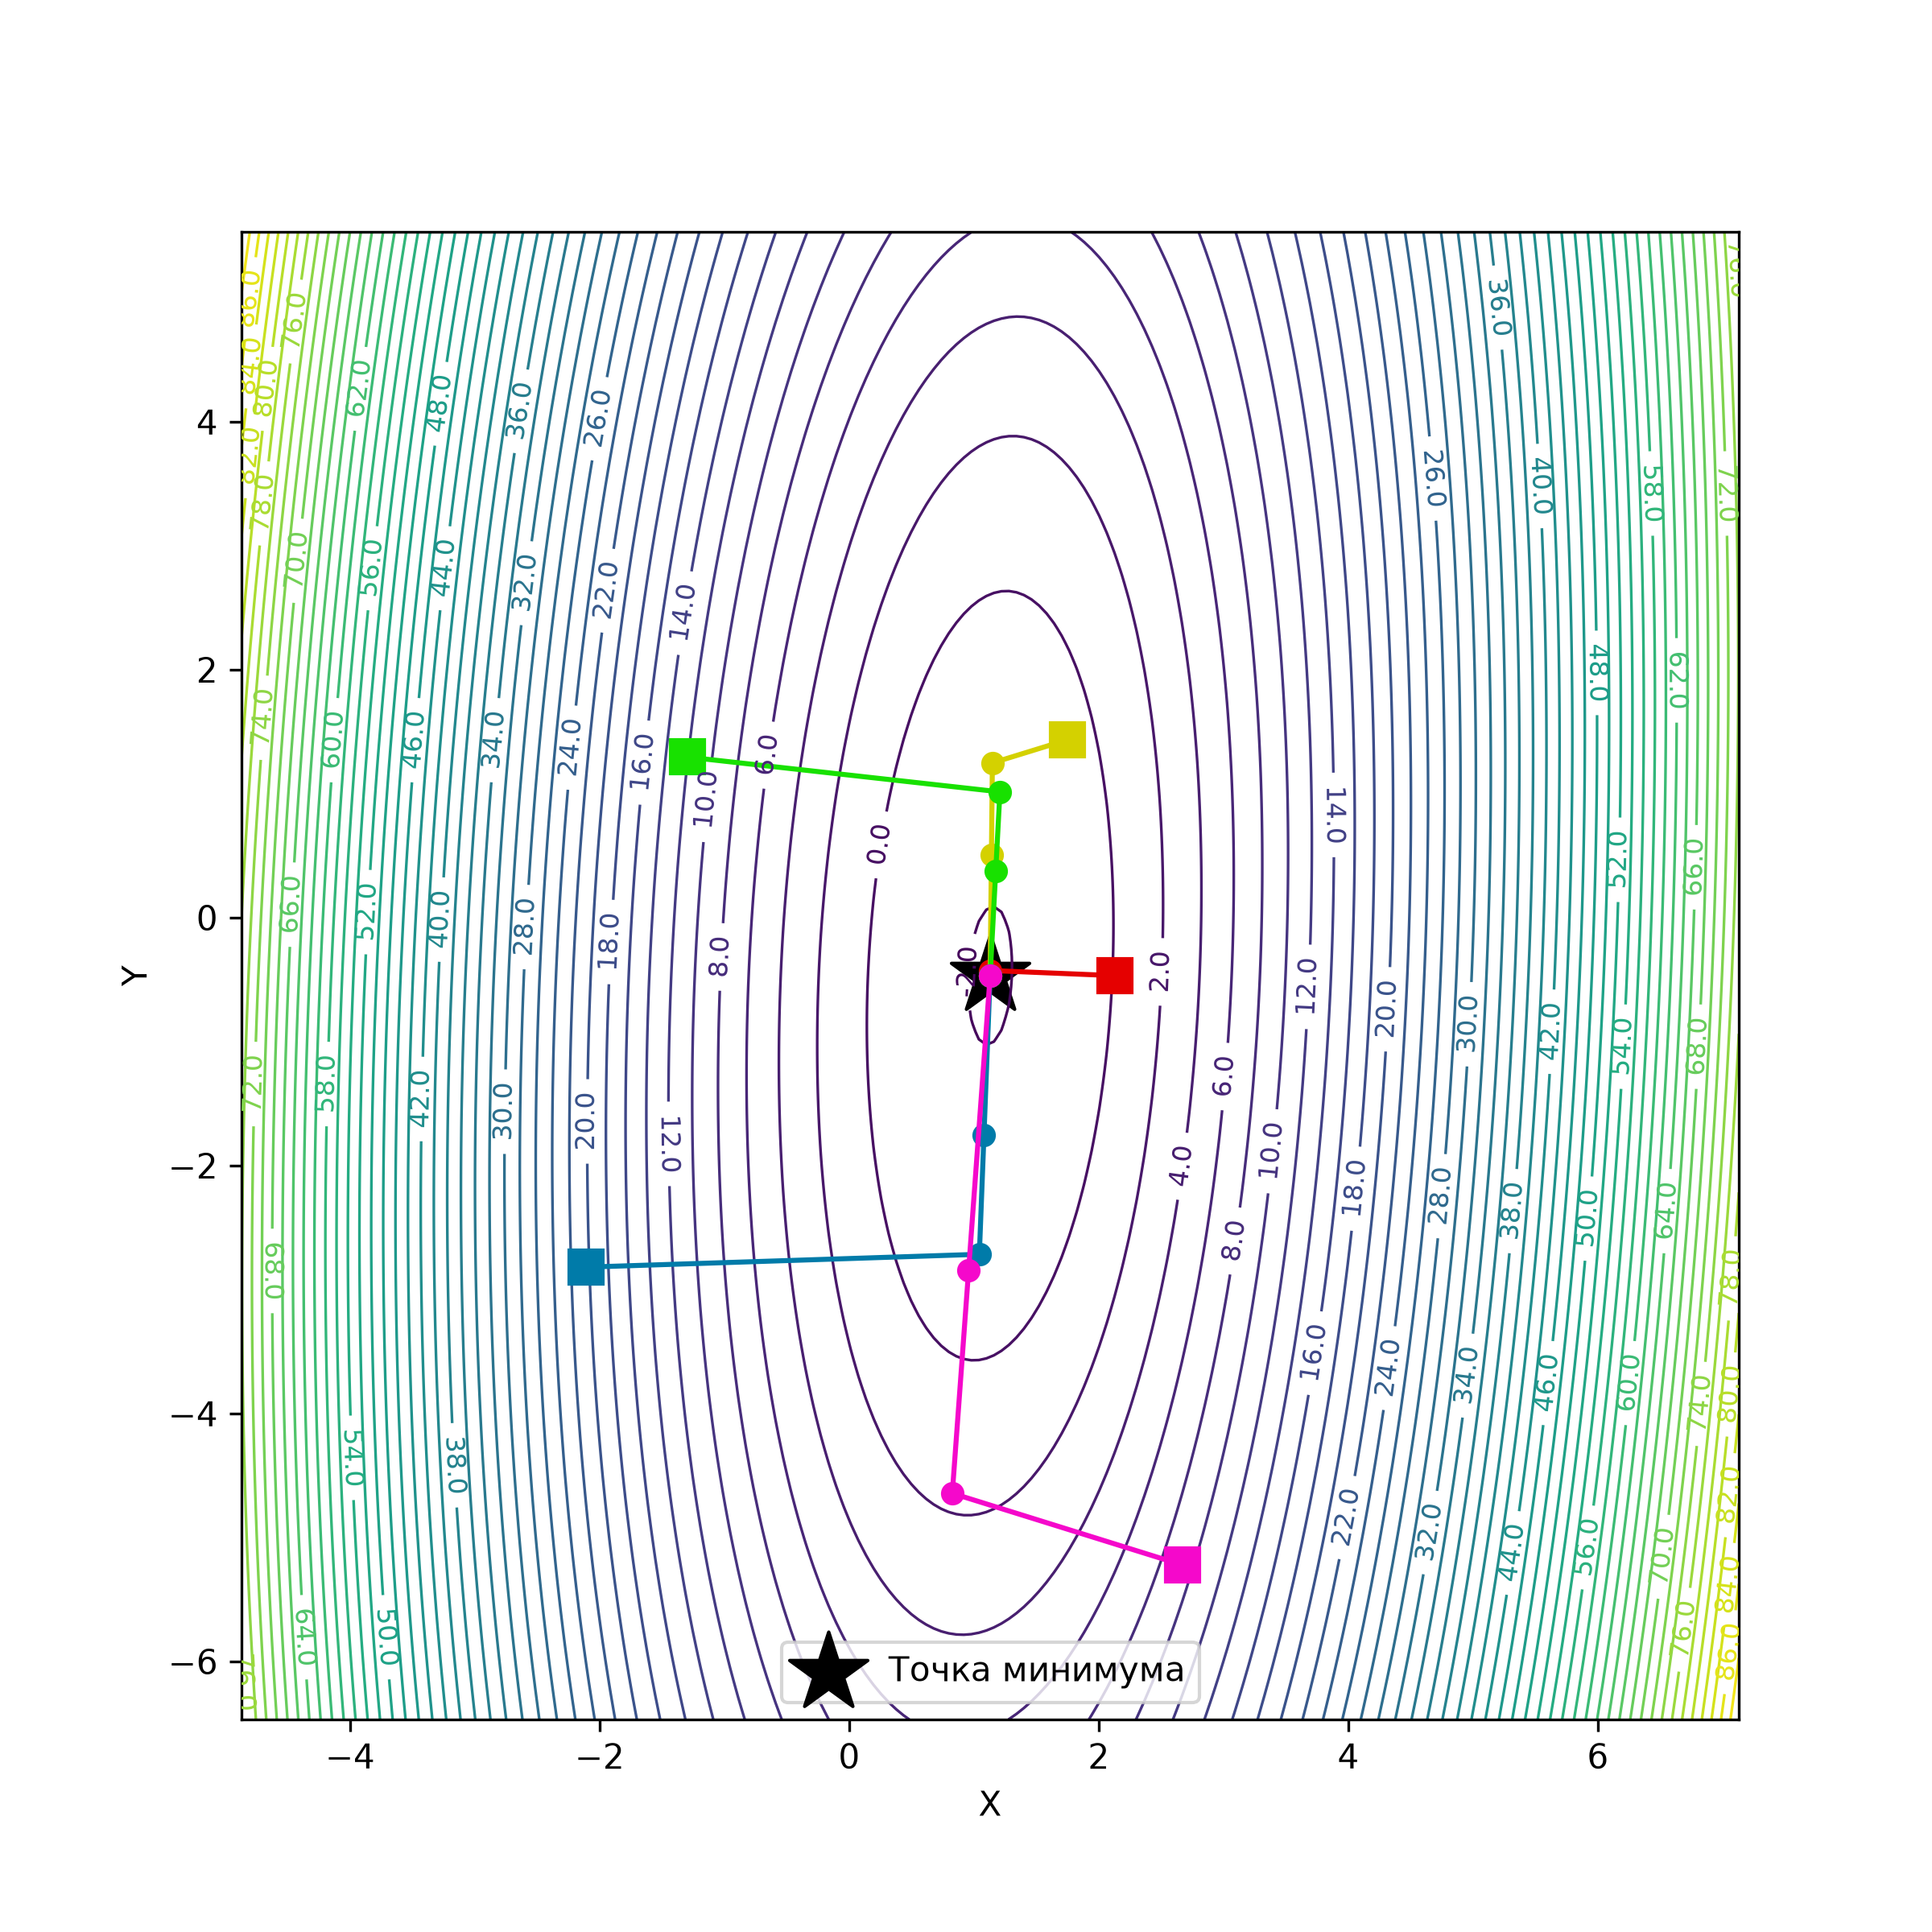
\includegraphics[width=0.3\textwidth]{task2_DFP_plot.png}}%
\hfill % <-- Seperation
\subcaptionbox{BFGS}{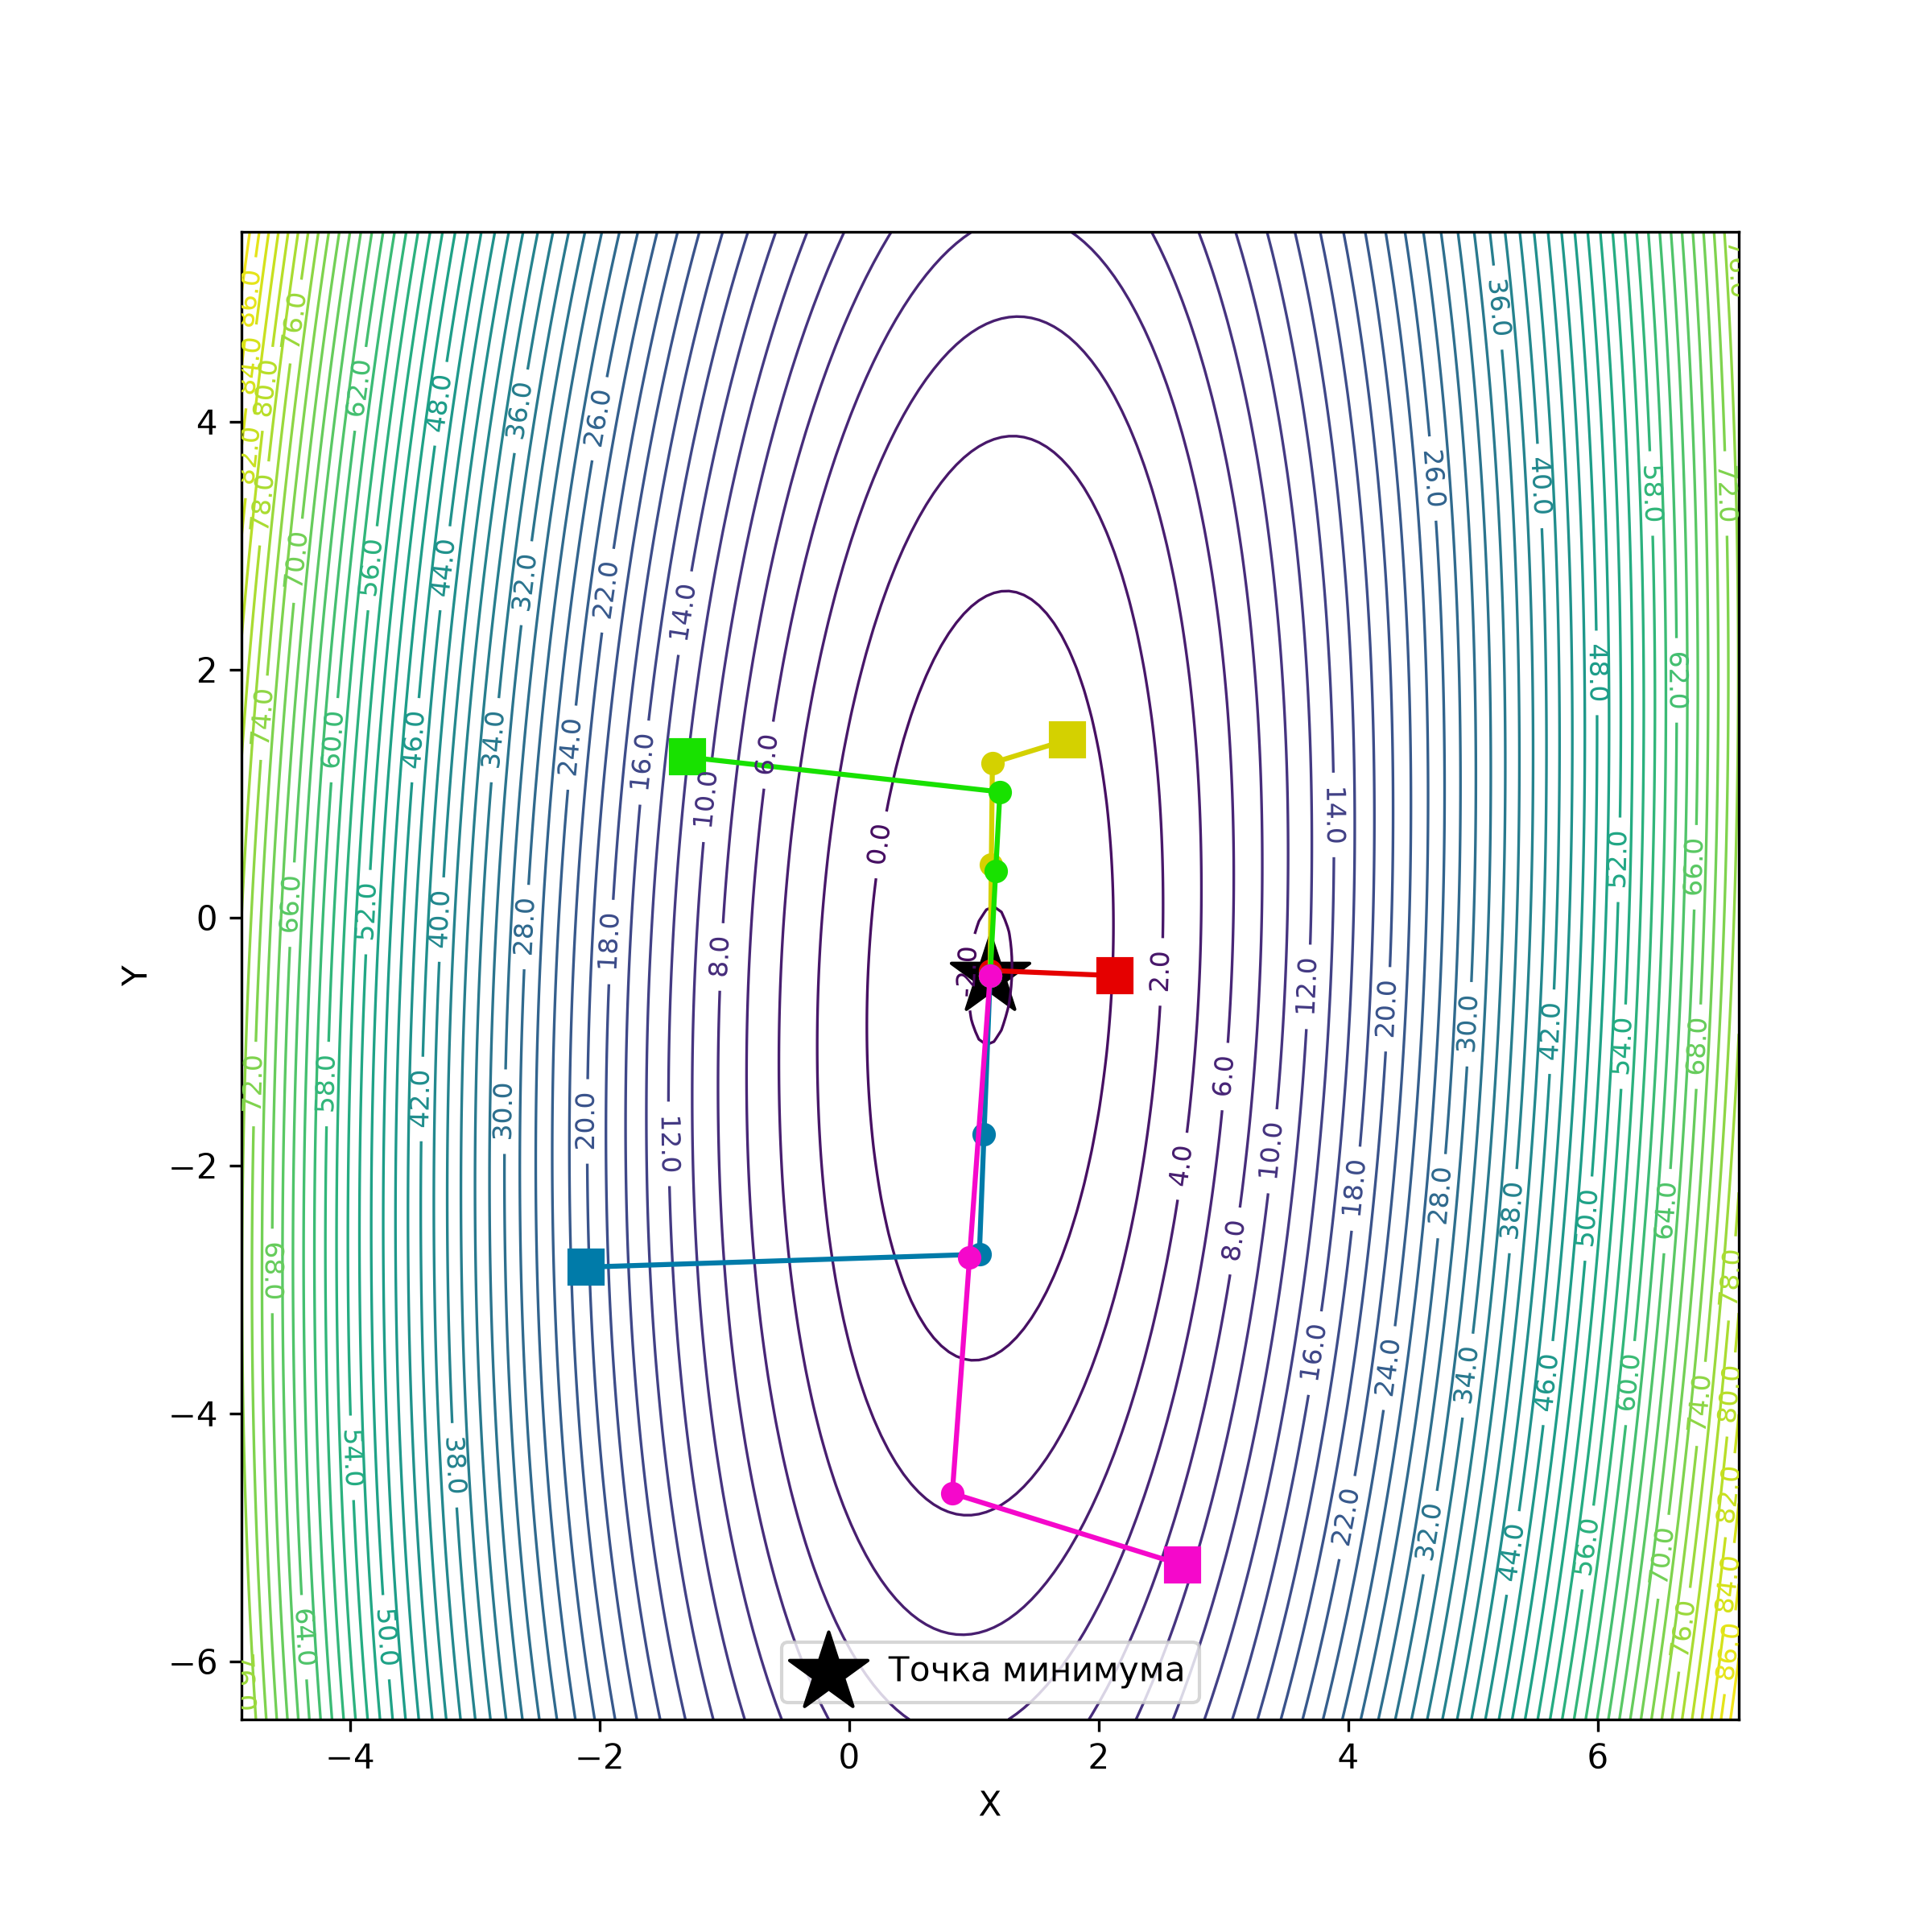
\includegraphics[width=0.3\textwidth]{task2_BFGS_plot.png}}%
\hfill % <-- Seperation
\subcaptionbox{L-BFGS}{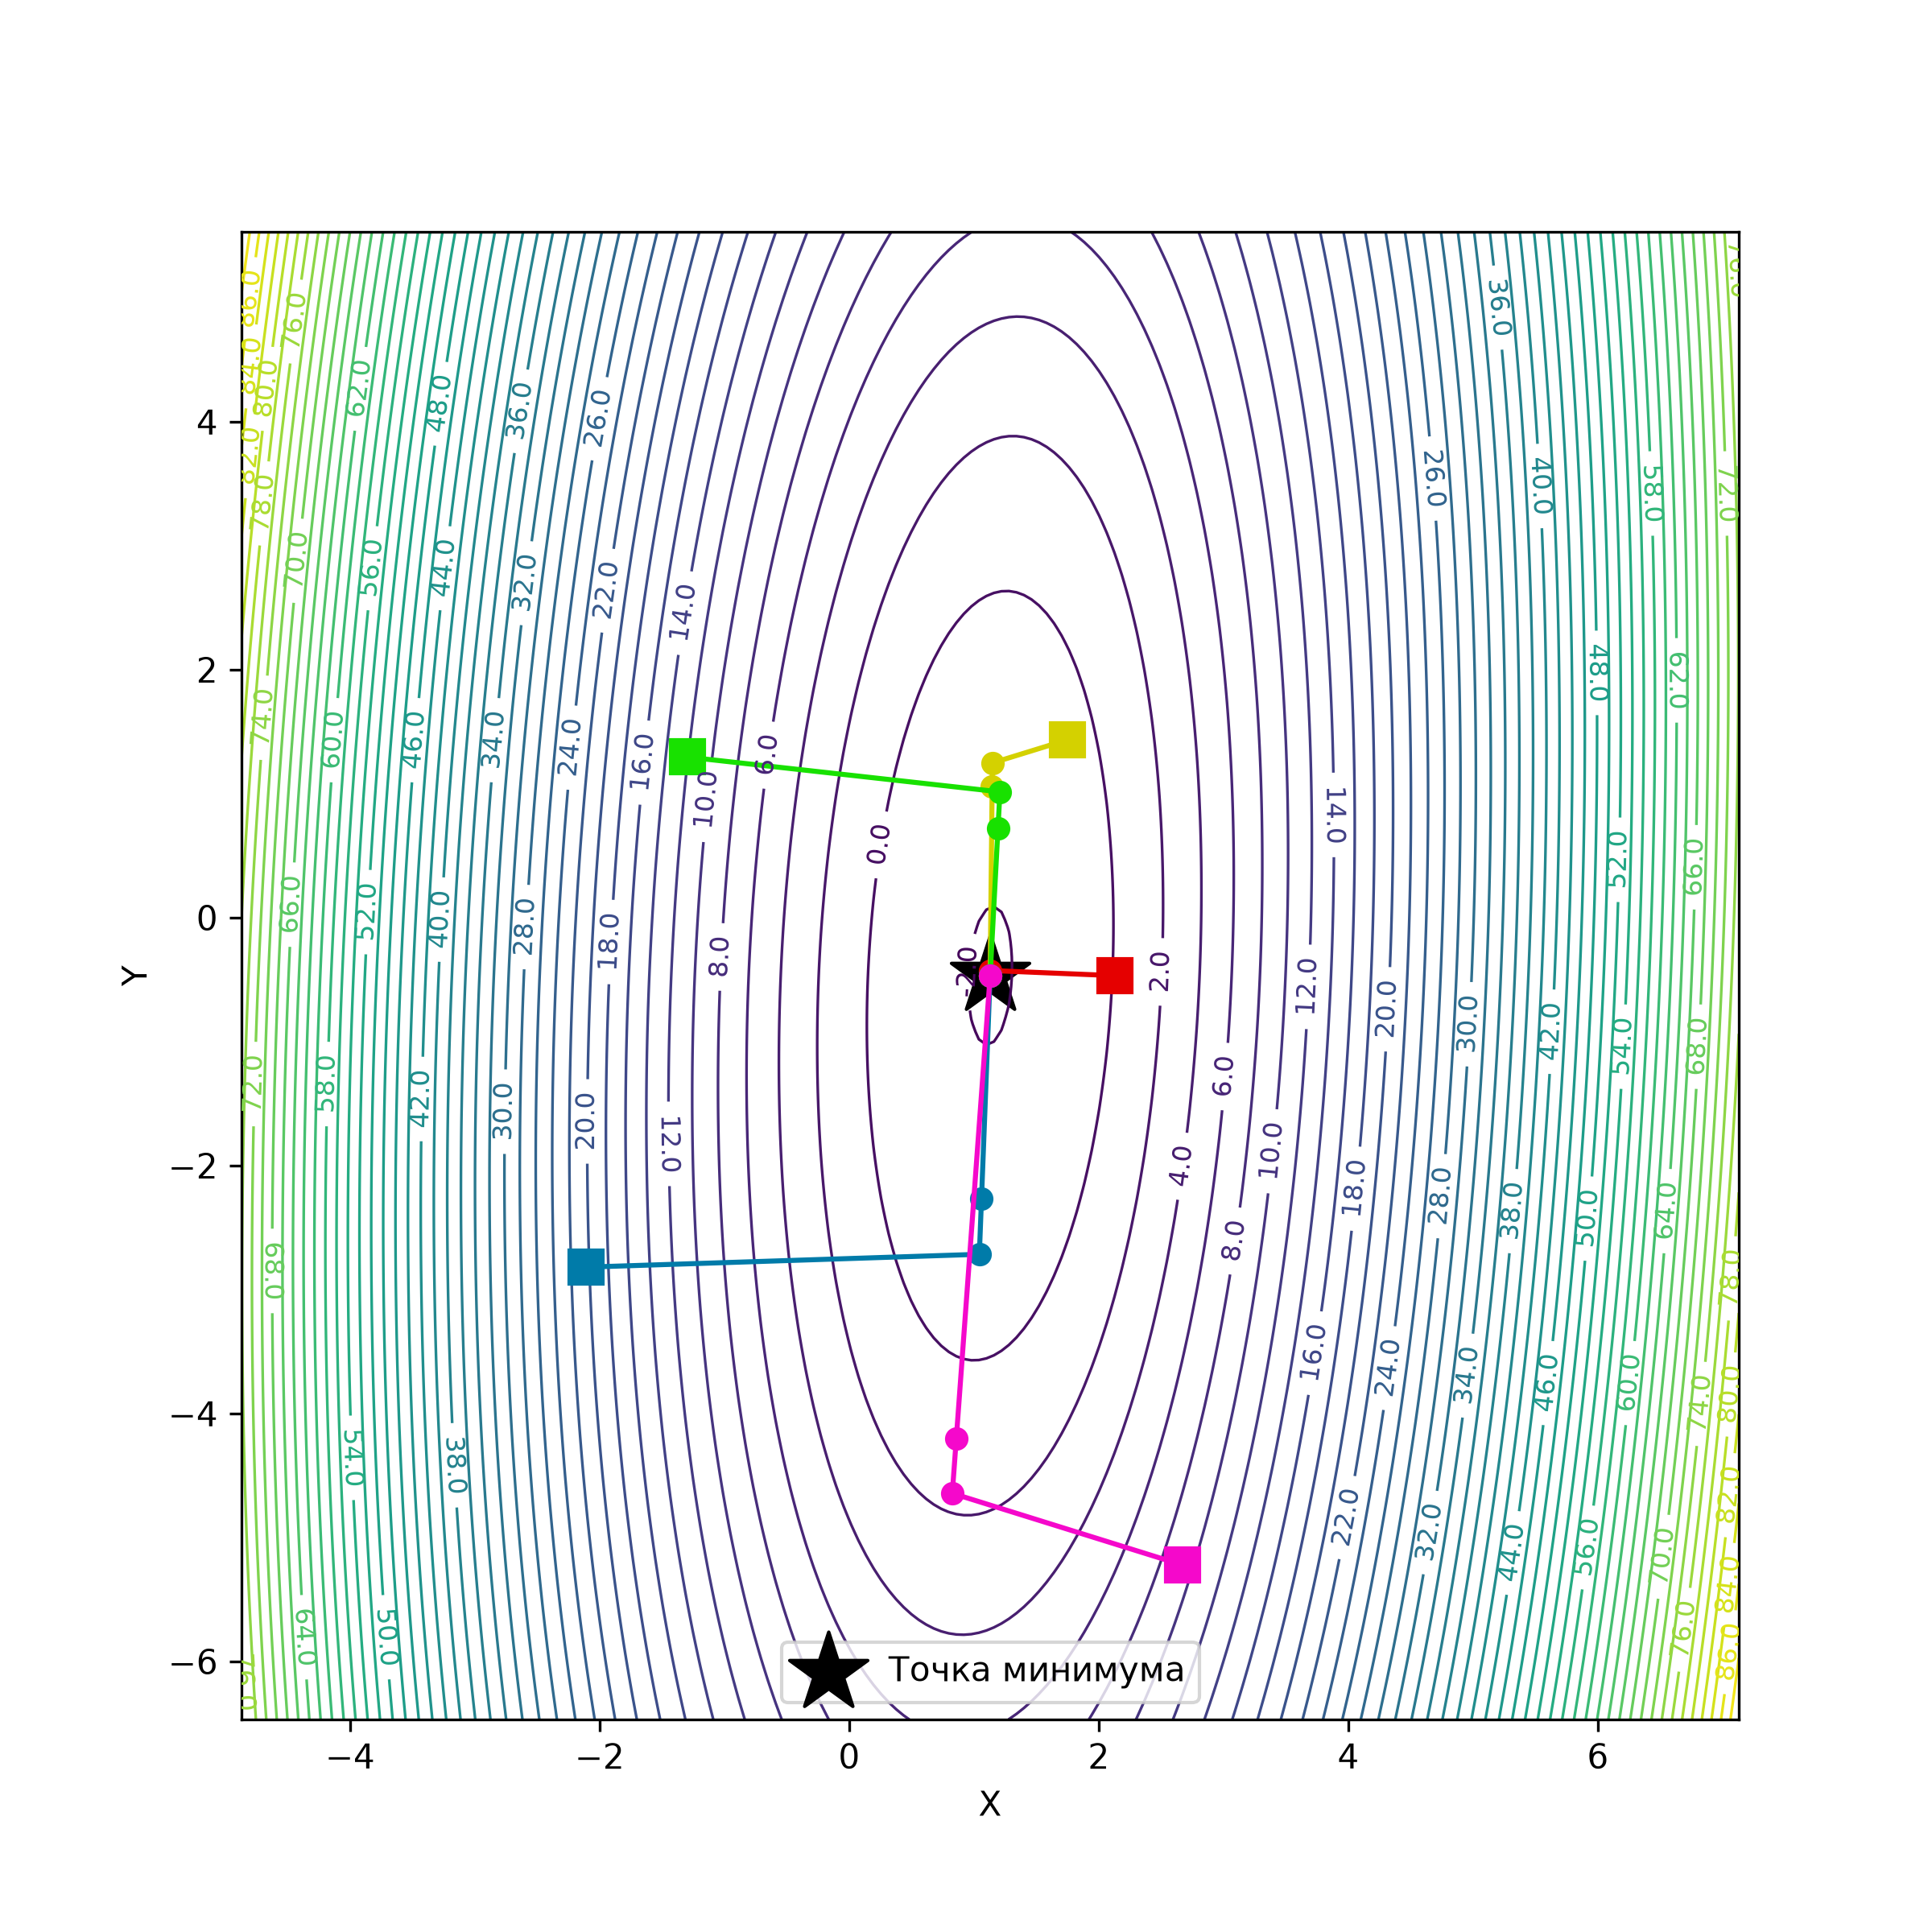
\includegraphics[width=0.3\textwidth]{task2_LBFGS_plot.png}}%
\\ % <-- Line break

\caption{Работа оптимизаторов на примере квадратичной функции.}
\end{figure}

Примечательно, что методы Ньютона сразу находили искомый минимум, не пытаясь следовать градиентным направлениям, как это сделали другие методы. Также, ввиду особенностей функции, видно, что дальнейшие направления спуска были сонаправлены с направлением градиентного спуска.


\subsection{Сходимость для сложных функций}

Были исследованы особенности сходимости оптимизаторов на примере сложных функций.

\begin{figure}[H]
\centering
\subcaptionbox{Сопр. градиенты}{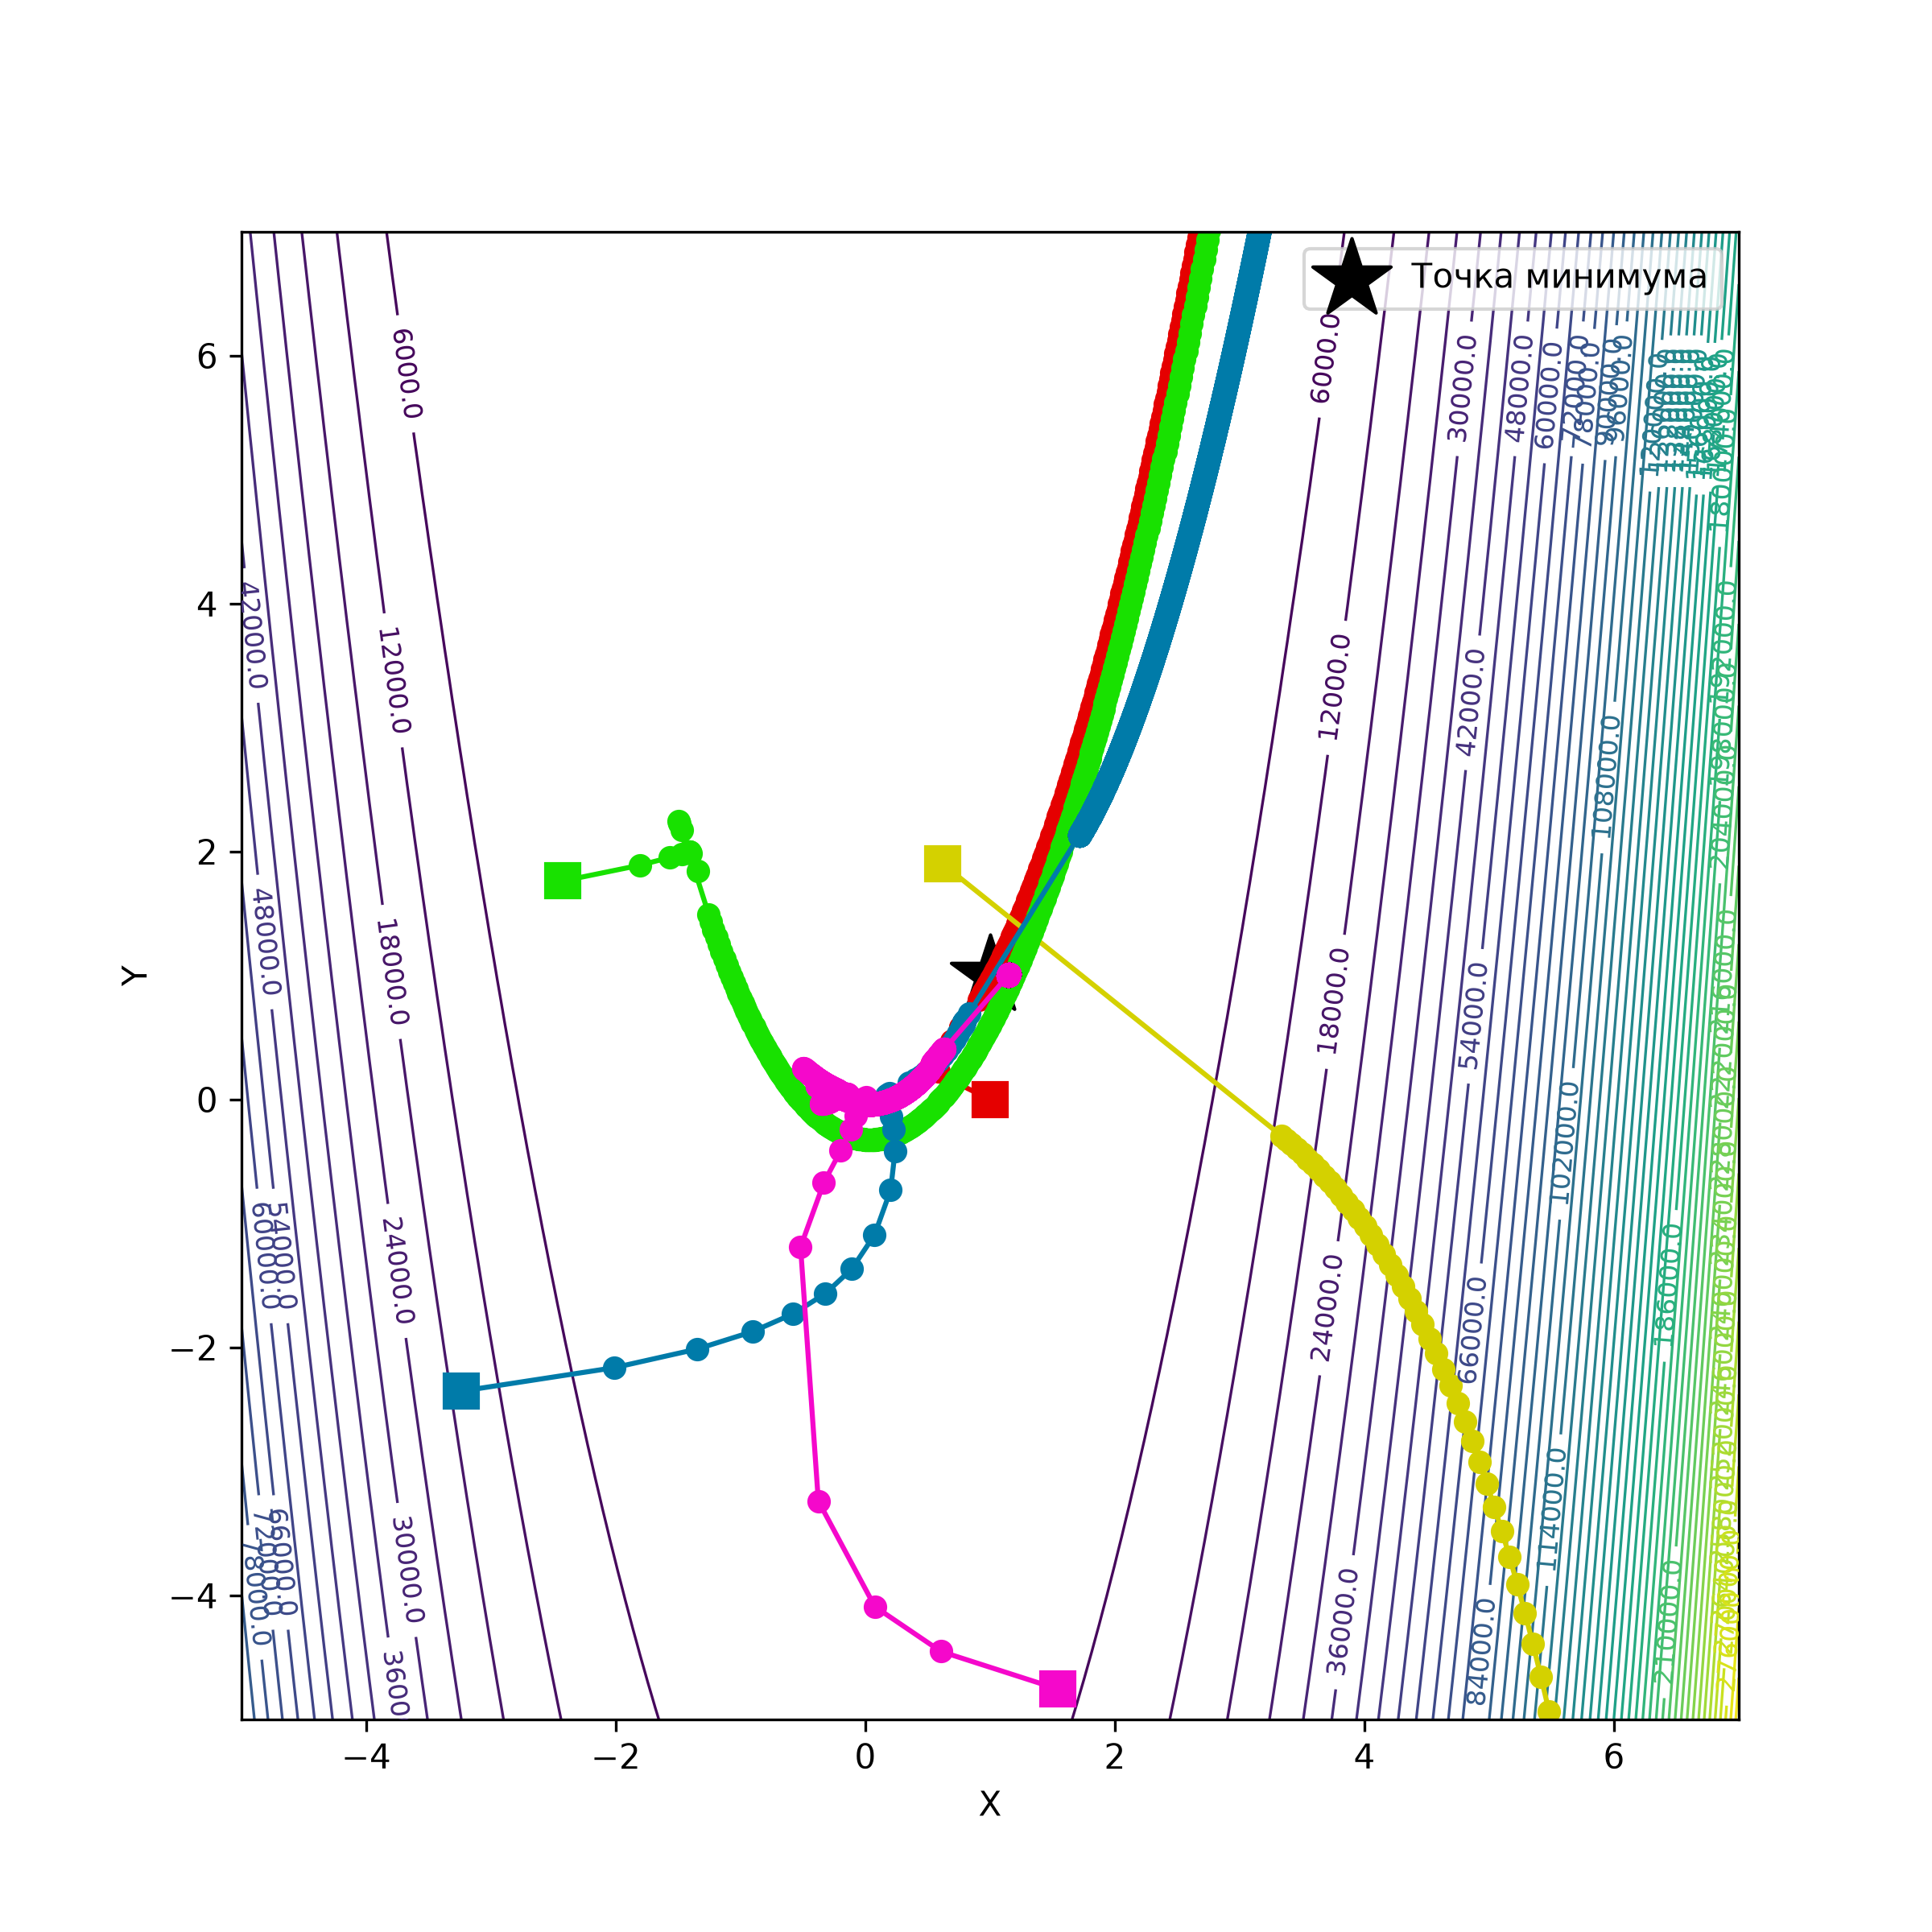
\includegraphics[width=0.3\textwidth]{task3_LinearConjugateGradient_Rosenbrock function_plot.png}}%
\hfill % <-- Seperation
\subcaptionbox{Флетчер-Ривс}{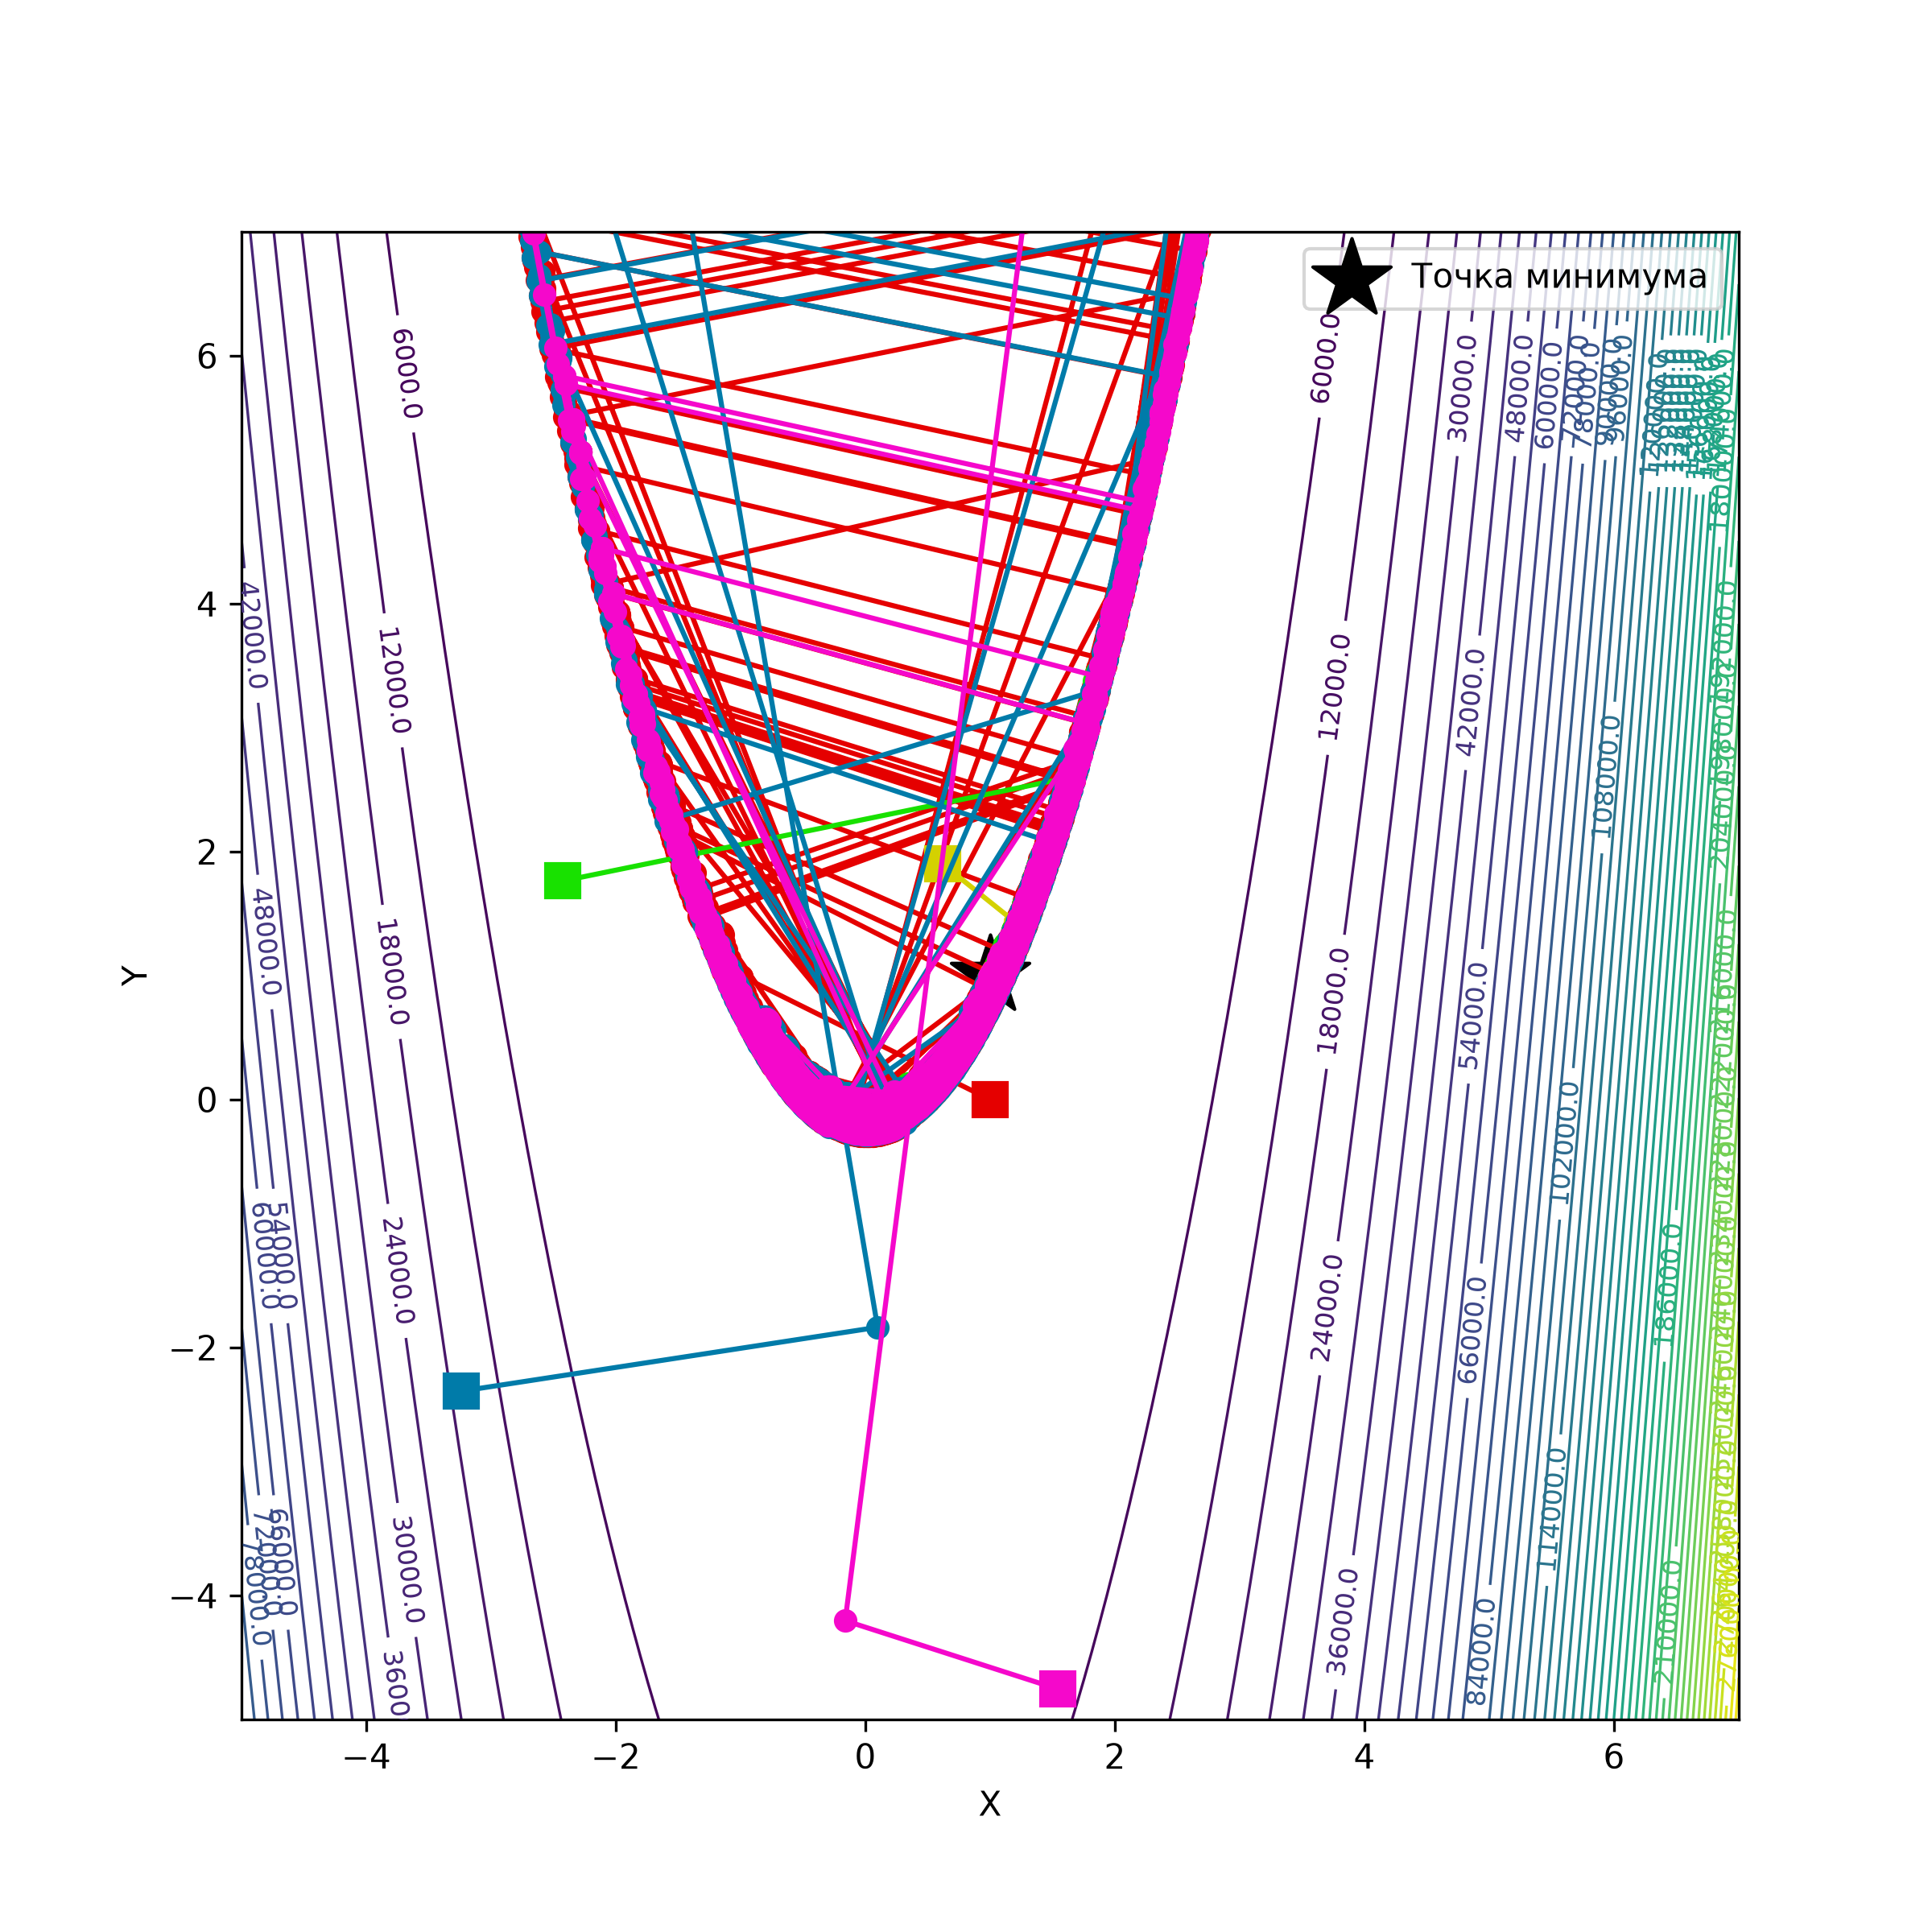
\includegraphics[width=0.3\textwidth]{task3_FletcherReeves_Rosenbrock function_plot.png}}%
\hfill % <-- Seperation
\subcaptionbox{Полак-Рибьер}{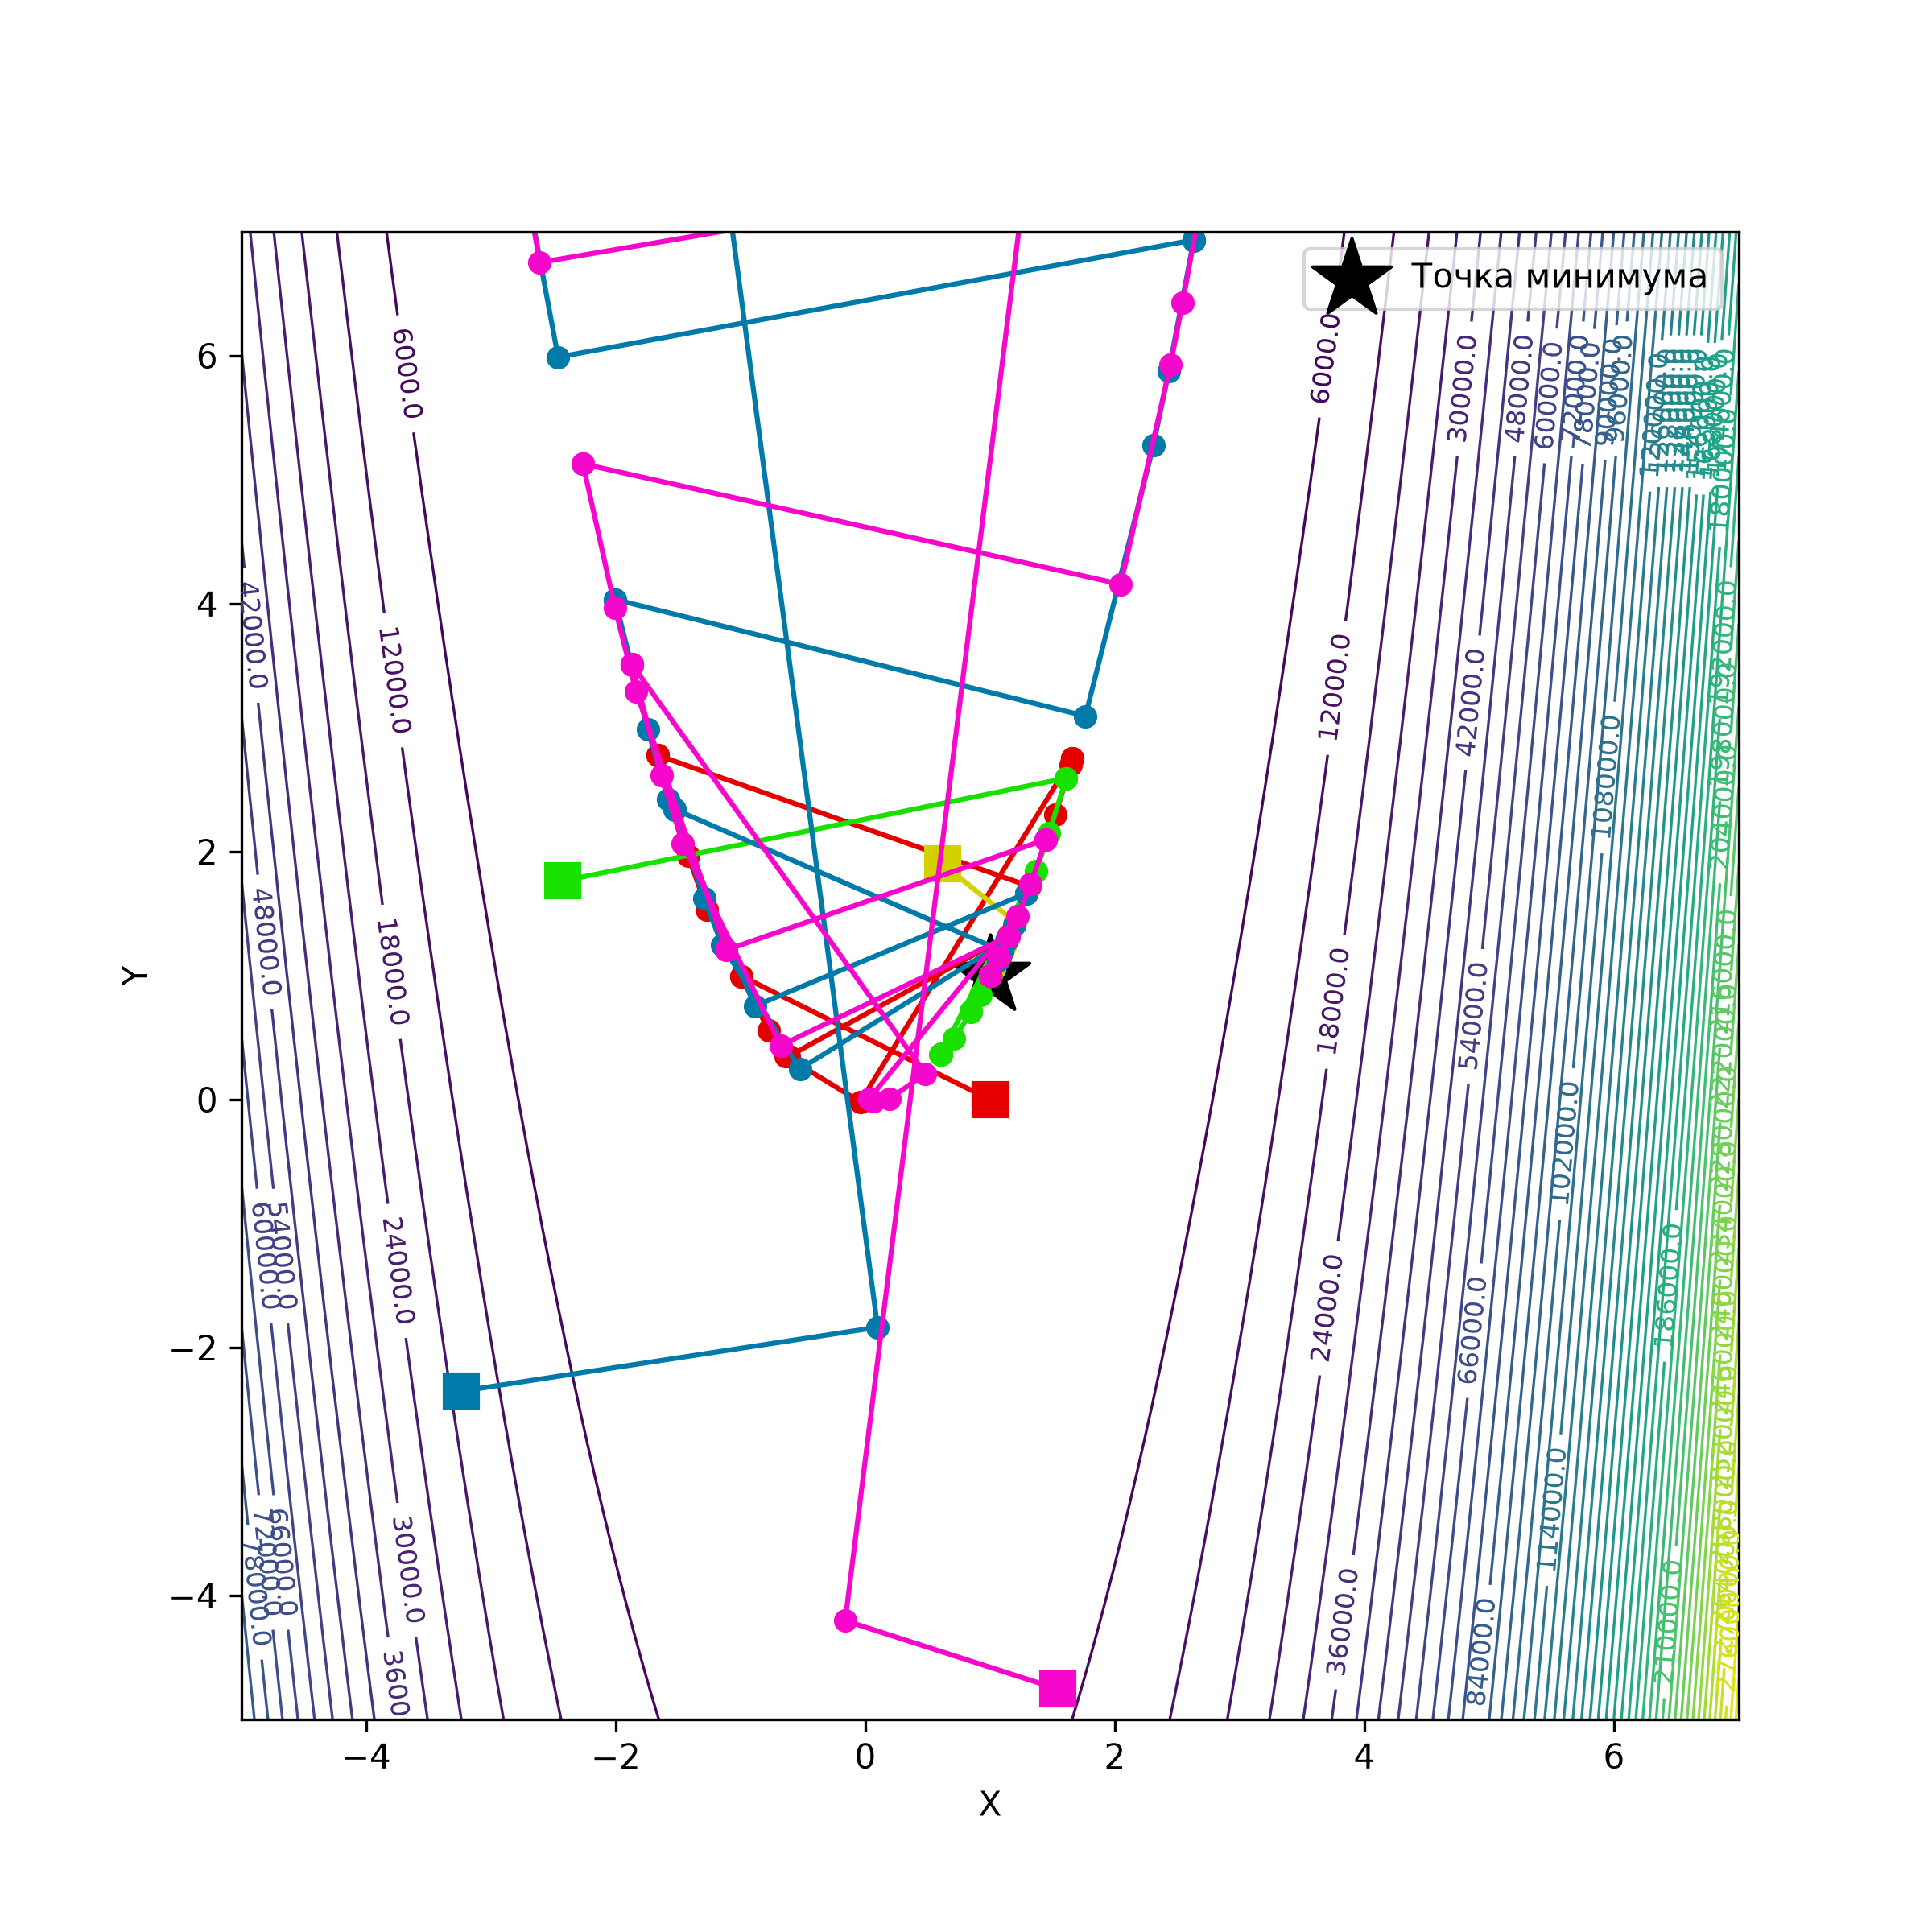
\includegraphics[width=0.3\textwidth]{task3_PolakRibiere_Rosenbrock function_plot.png}}%
\\ % <-- Line break
\centering
\subcaptionbox{Разл. Холецкого}{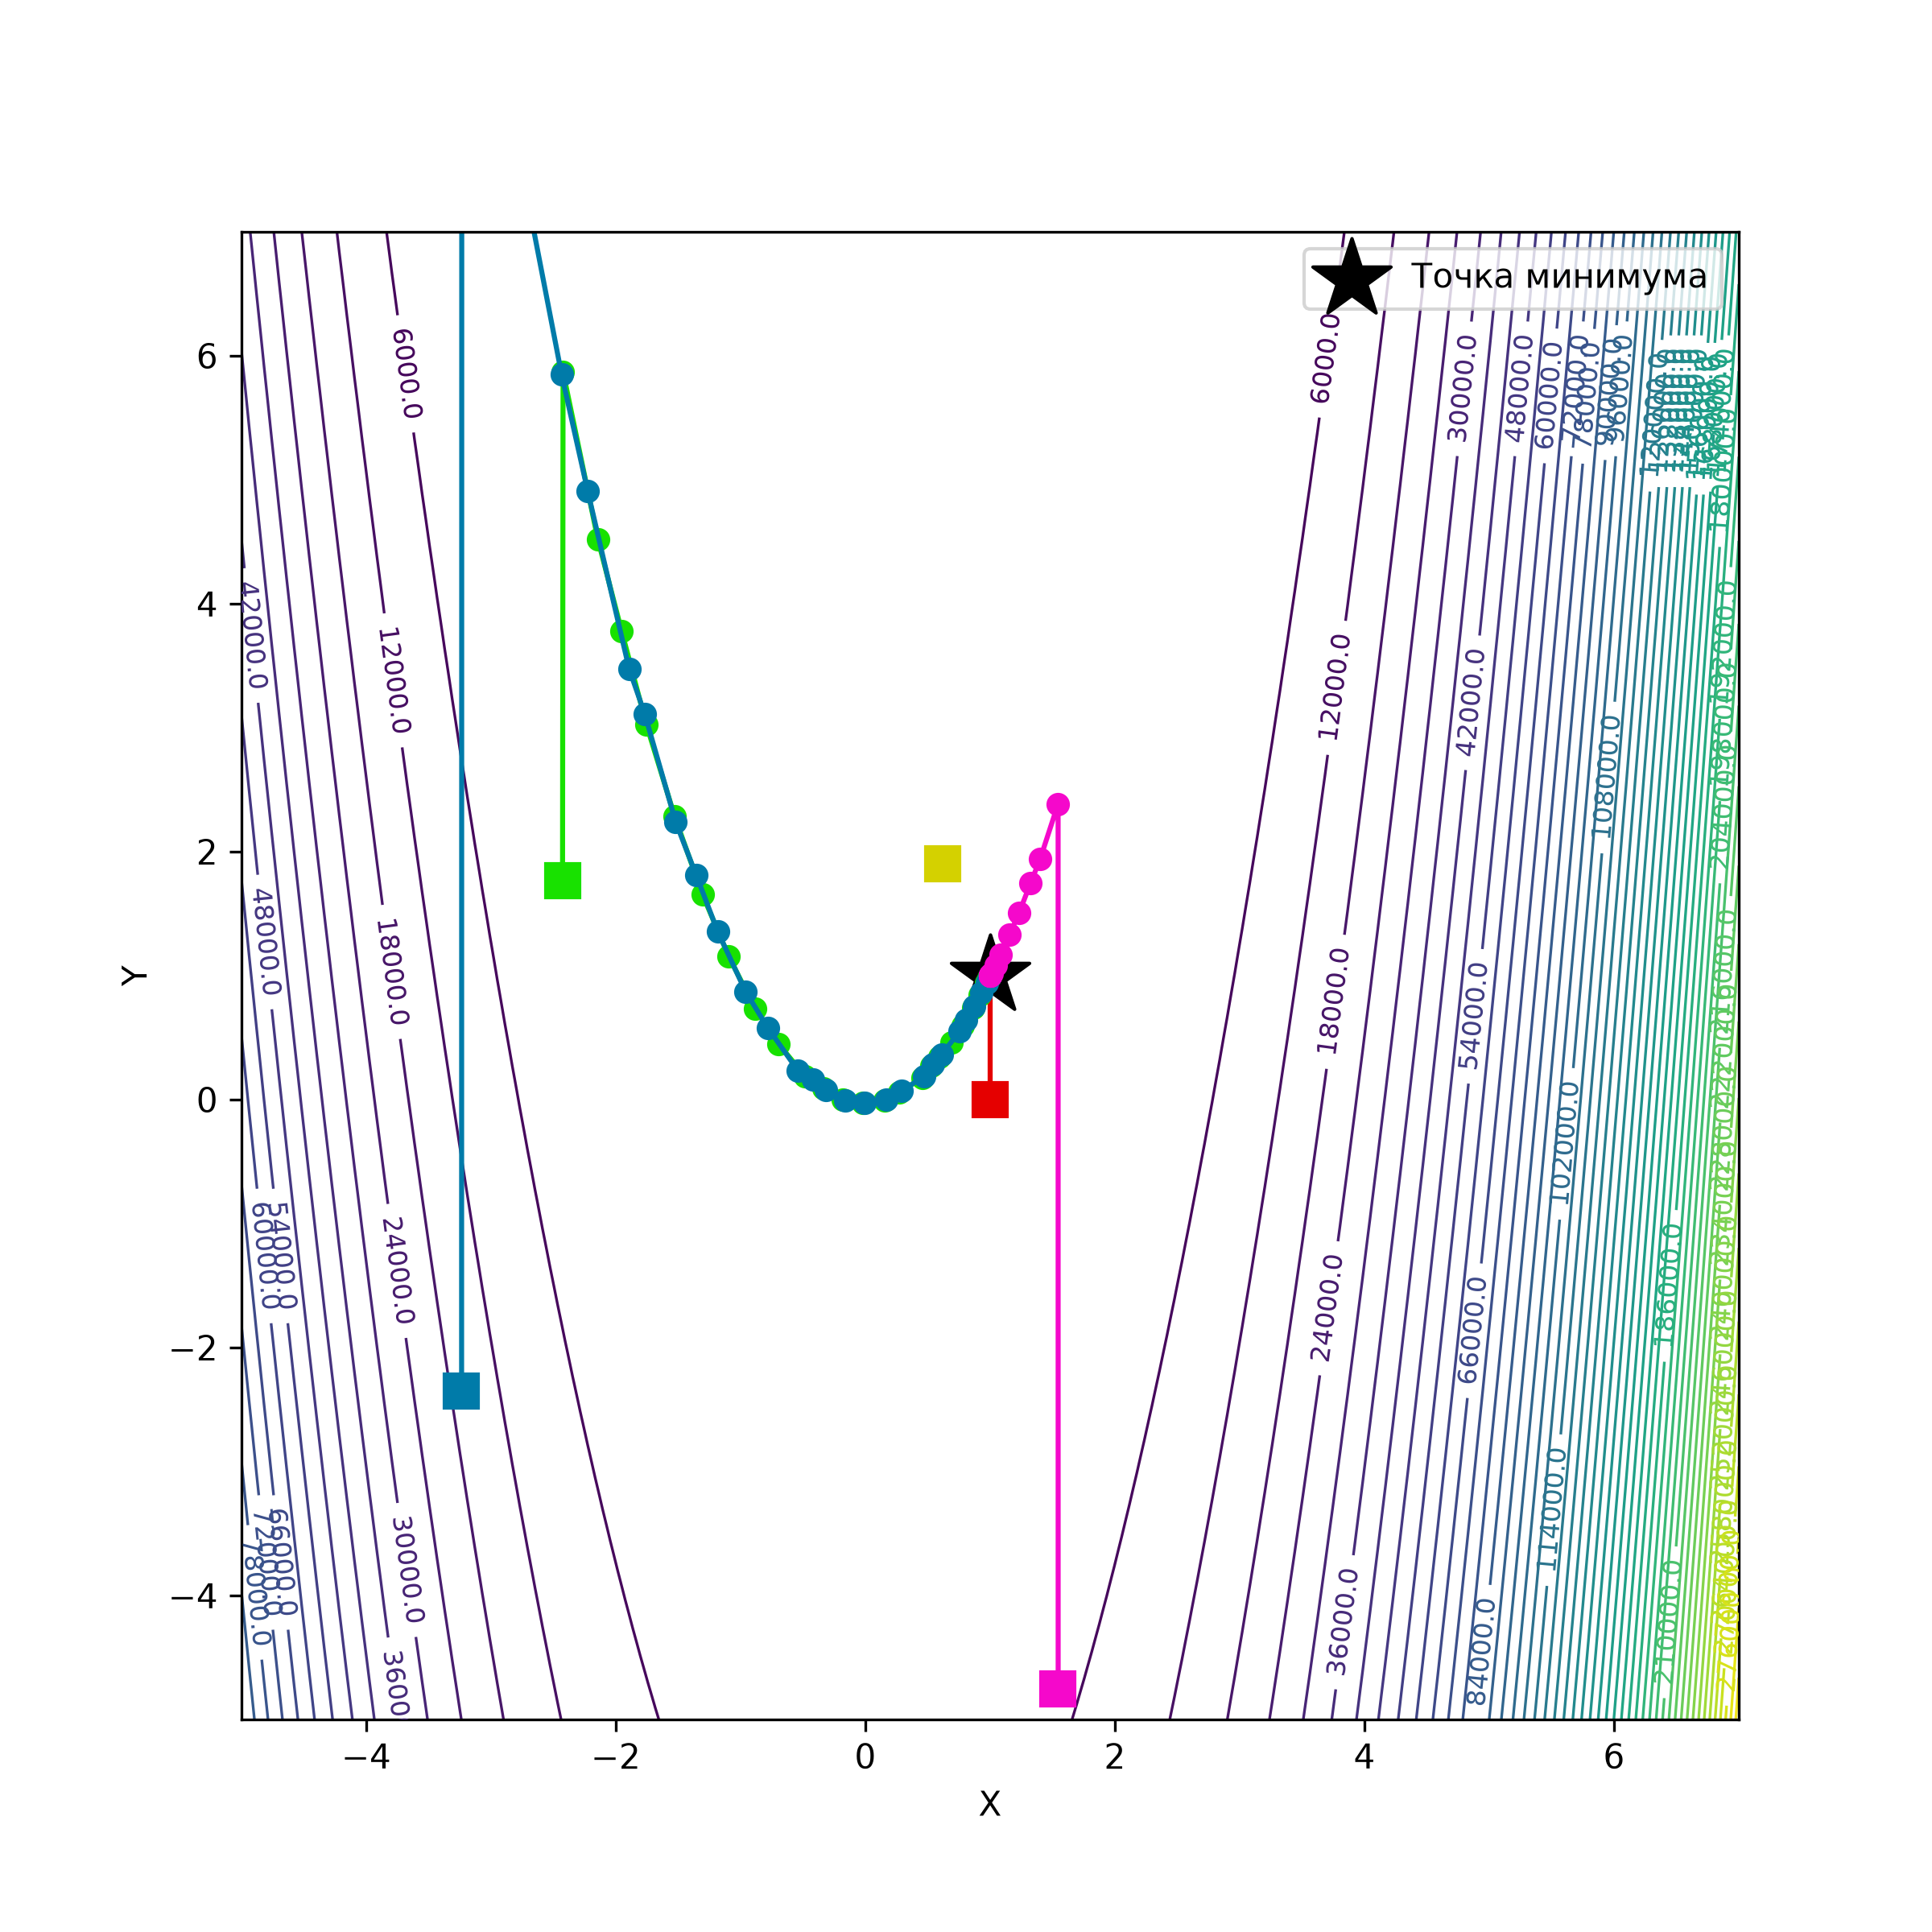
\includegraphics[width=0.3\textwidth]{task3_NewtonCholesky_Rosenbrock function_plot.png}}%
\hfill % <-- Seperation
\subcaptionbox{Выбор направления}{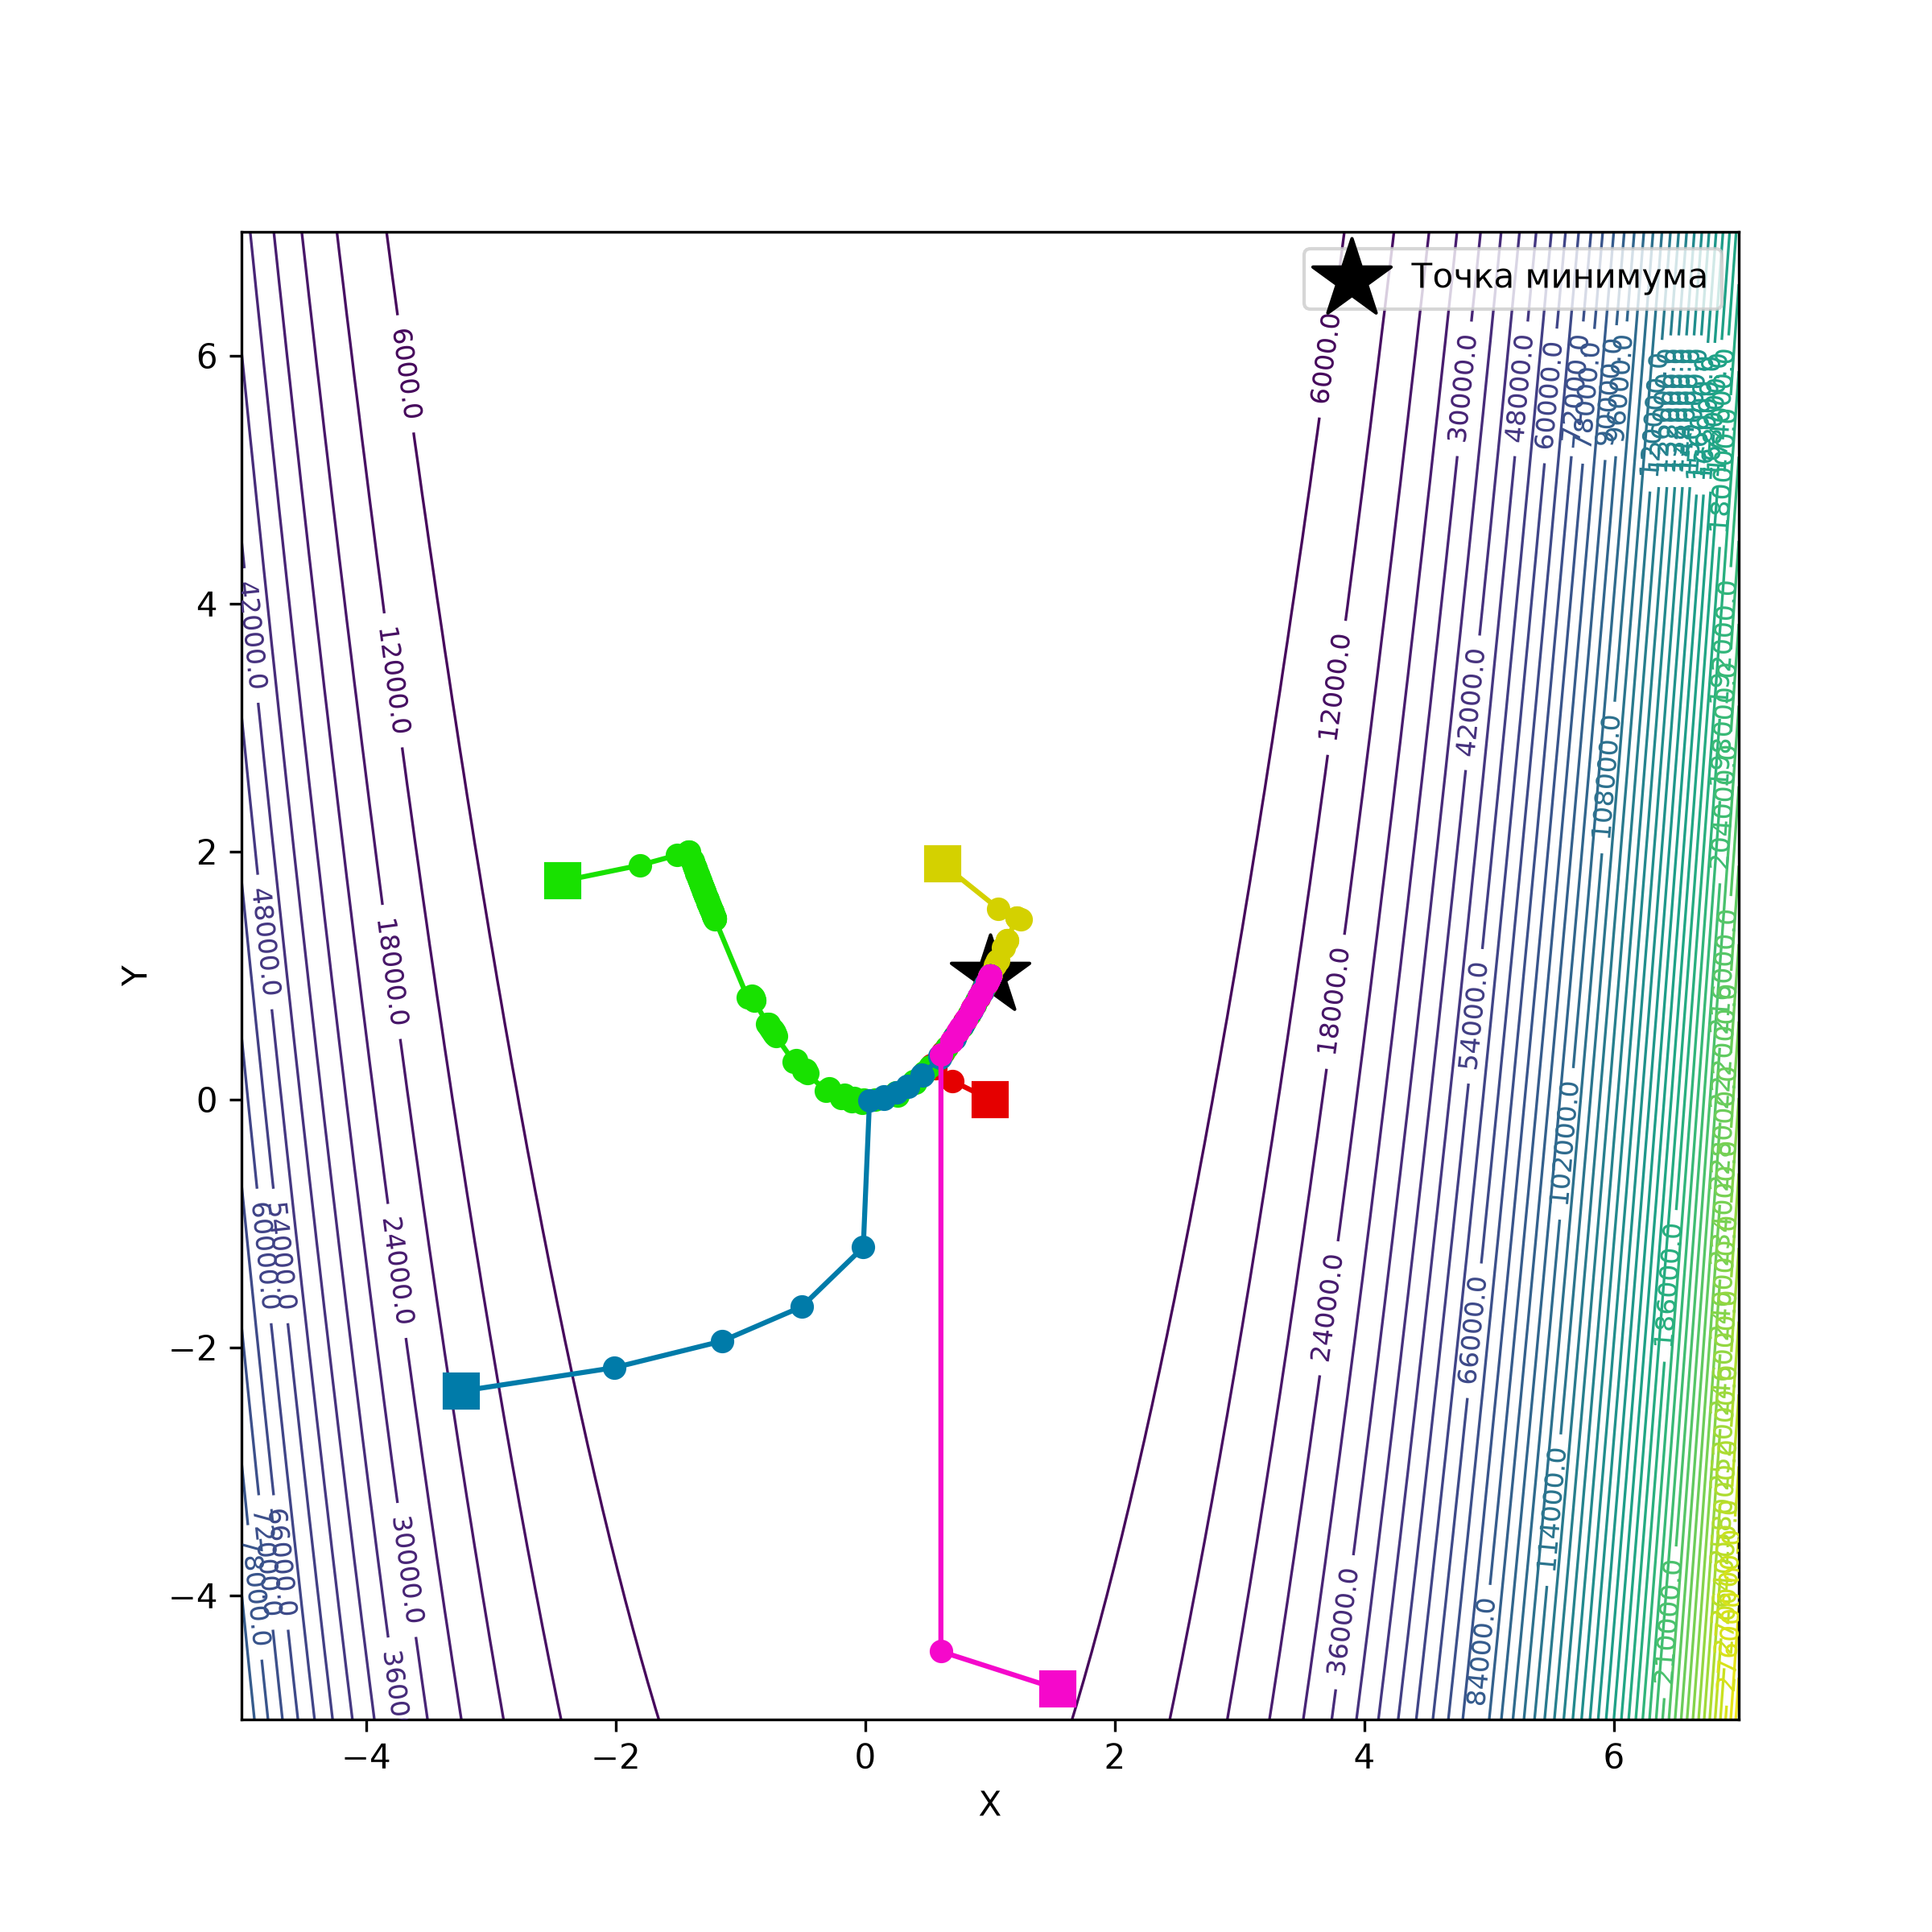
\includegraphics[width=0.3\textwidth]{task3_NewtonCG_Rosenbrock function_plot.png}}%
\hfill % <-- Seperation
\subcaptionbox{Powell's Dog Leg}{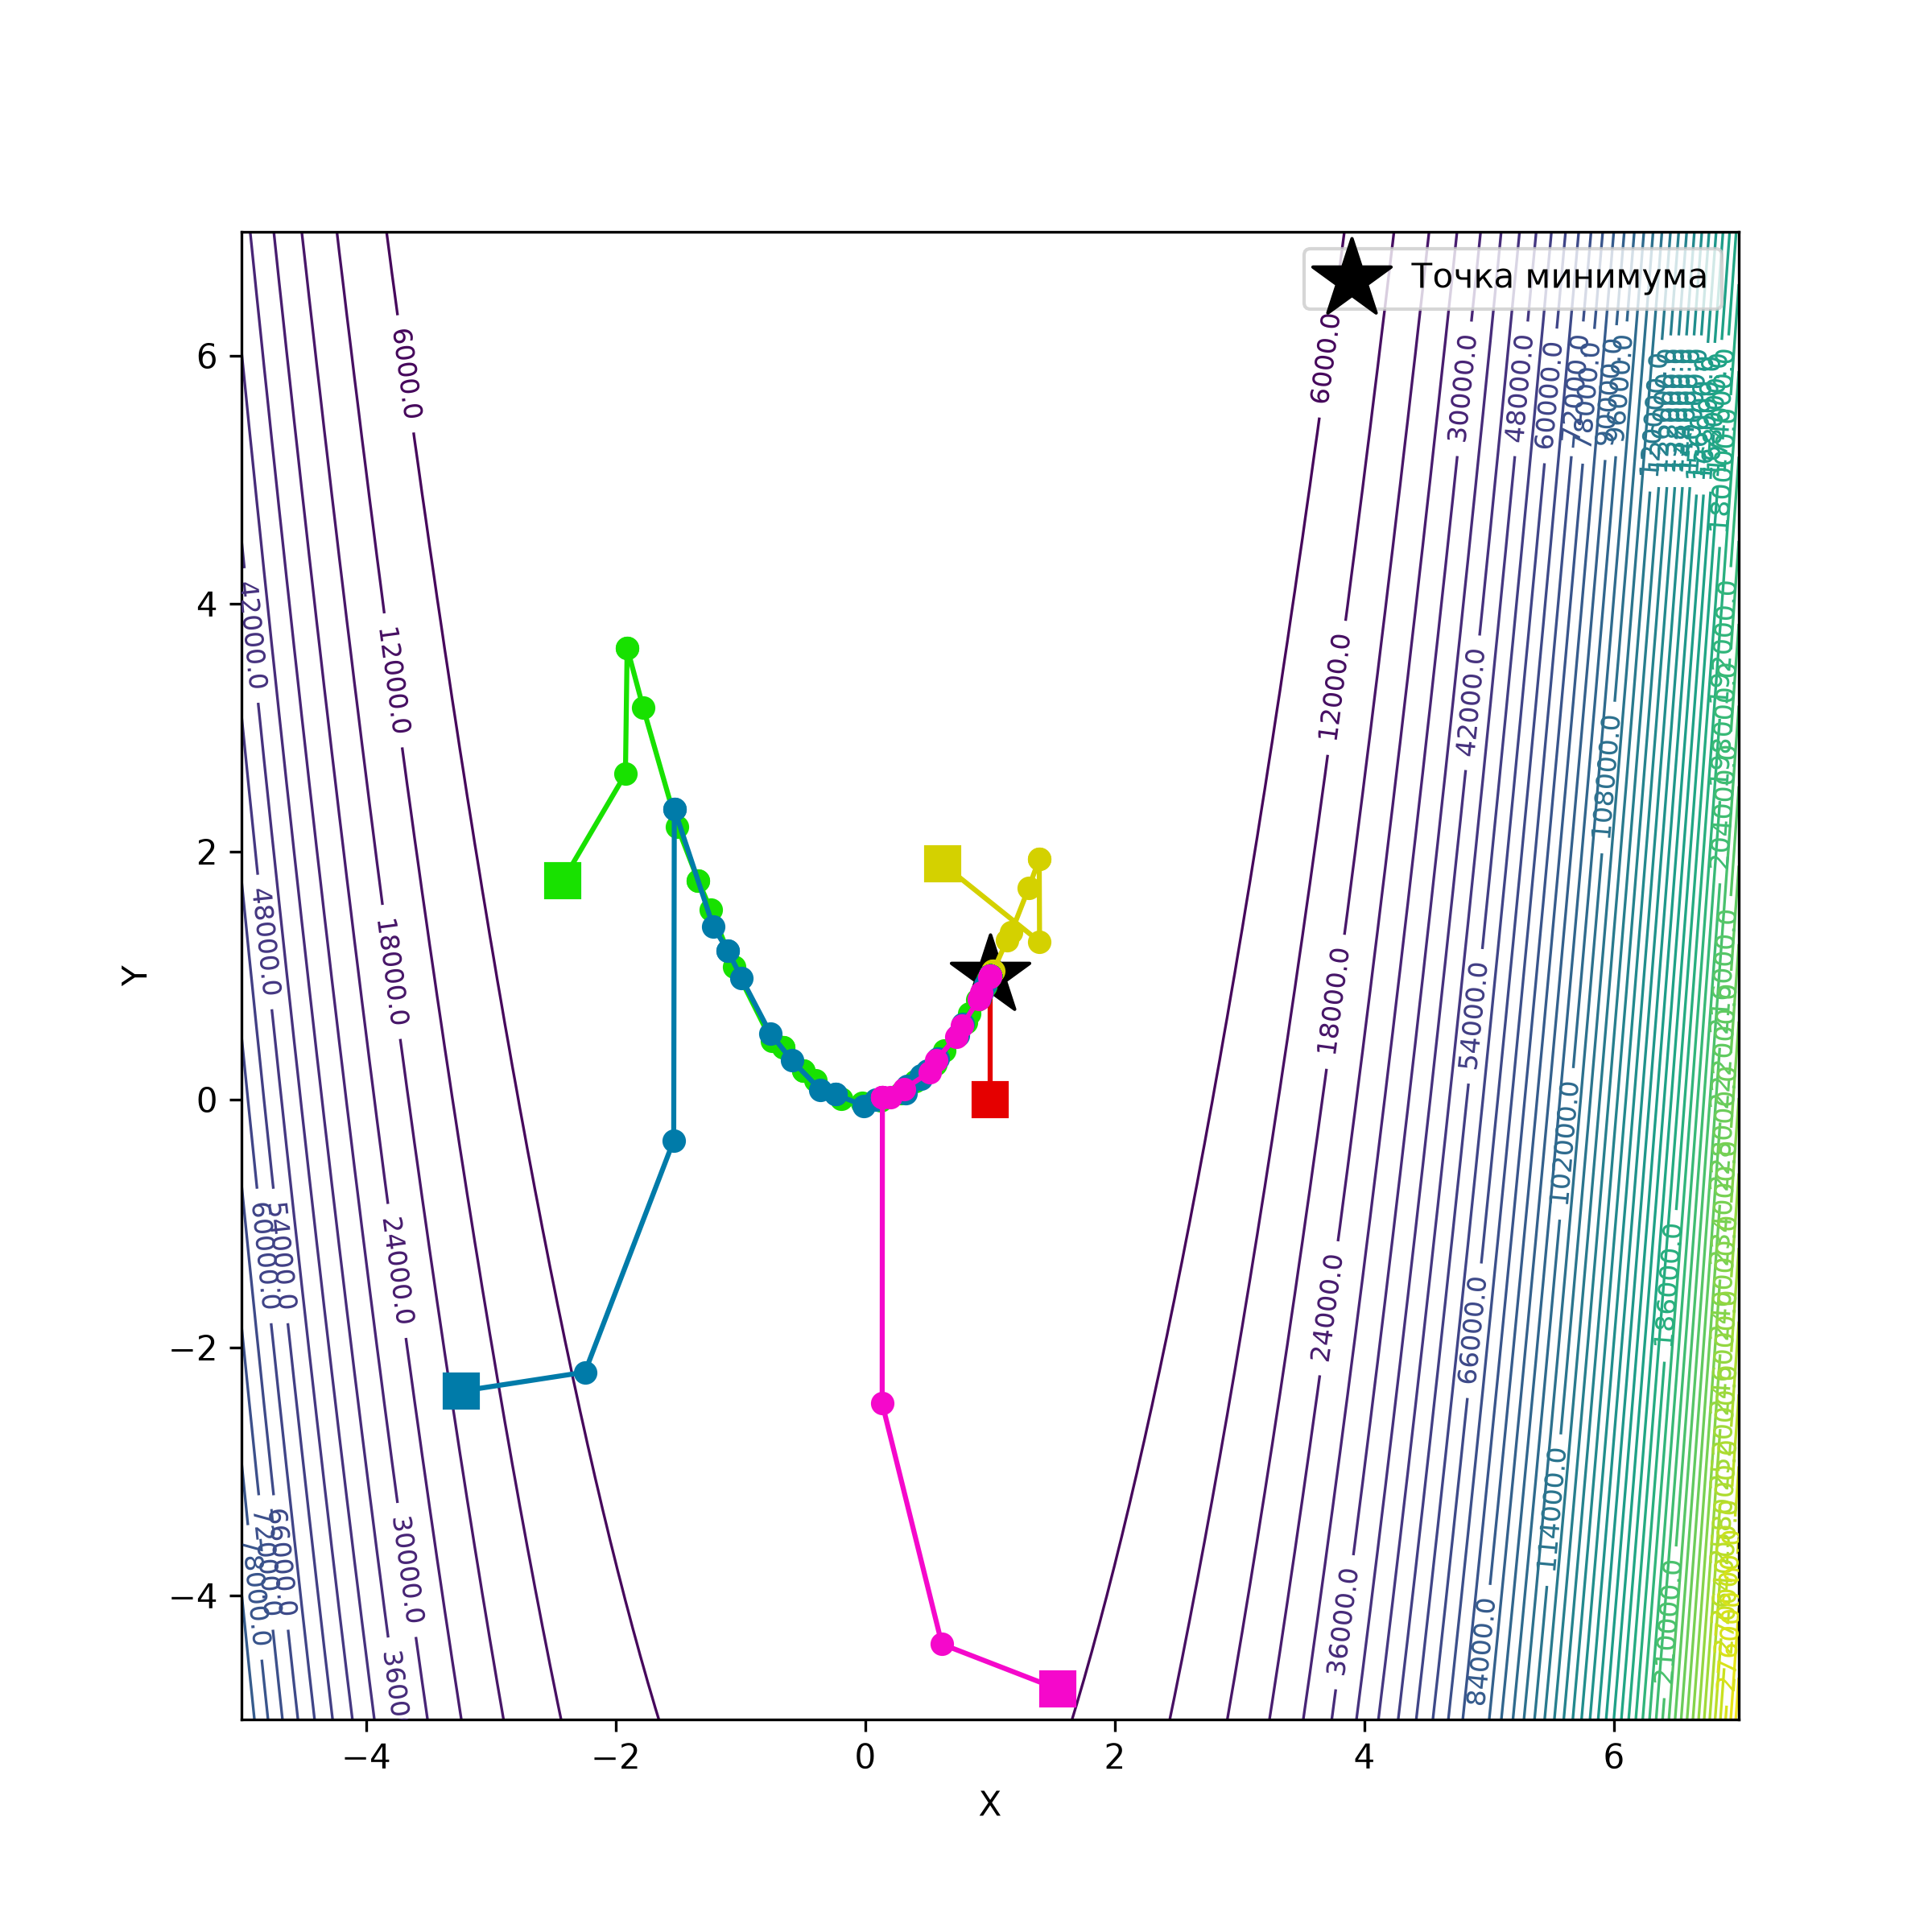
\includegraphics[width=0.3\textwidth]{task3_PowellsDogLeg_Rosenbrock function_plot.png}}%
\\ % <-- Line break
\centering
\subcaptionbox{DFP}{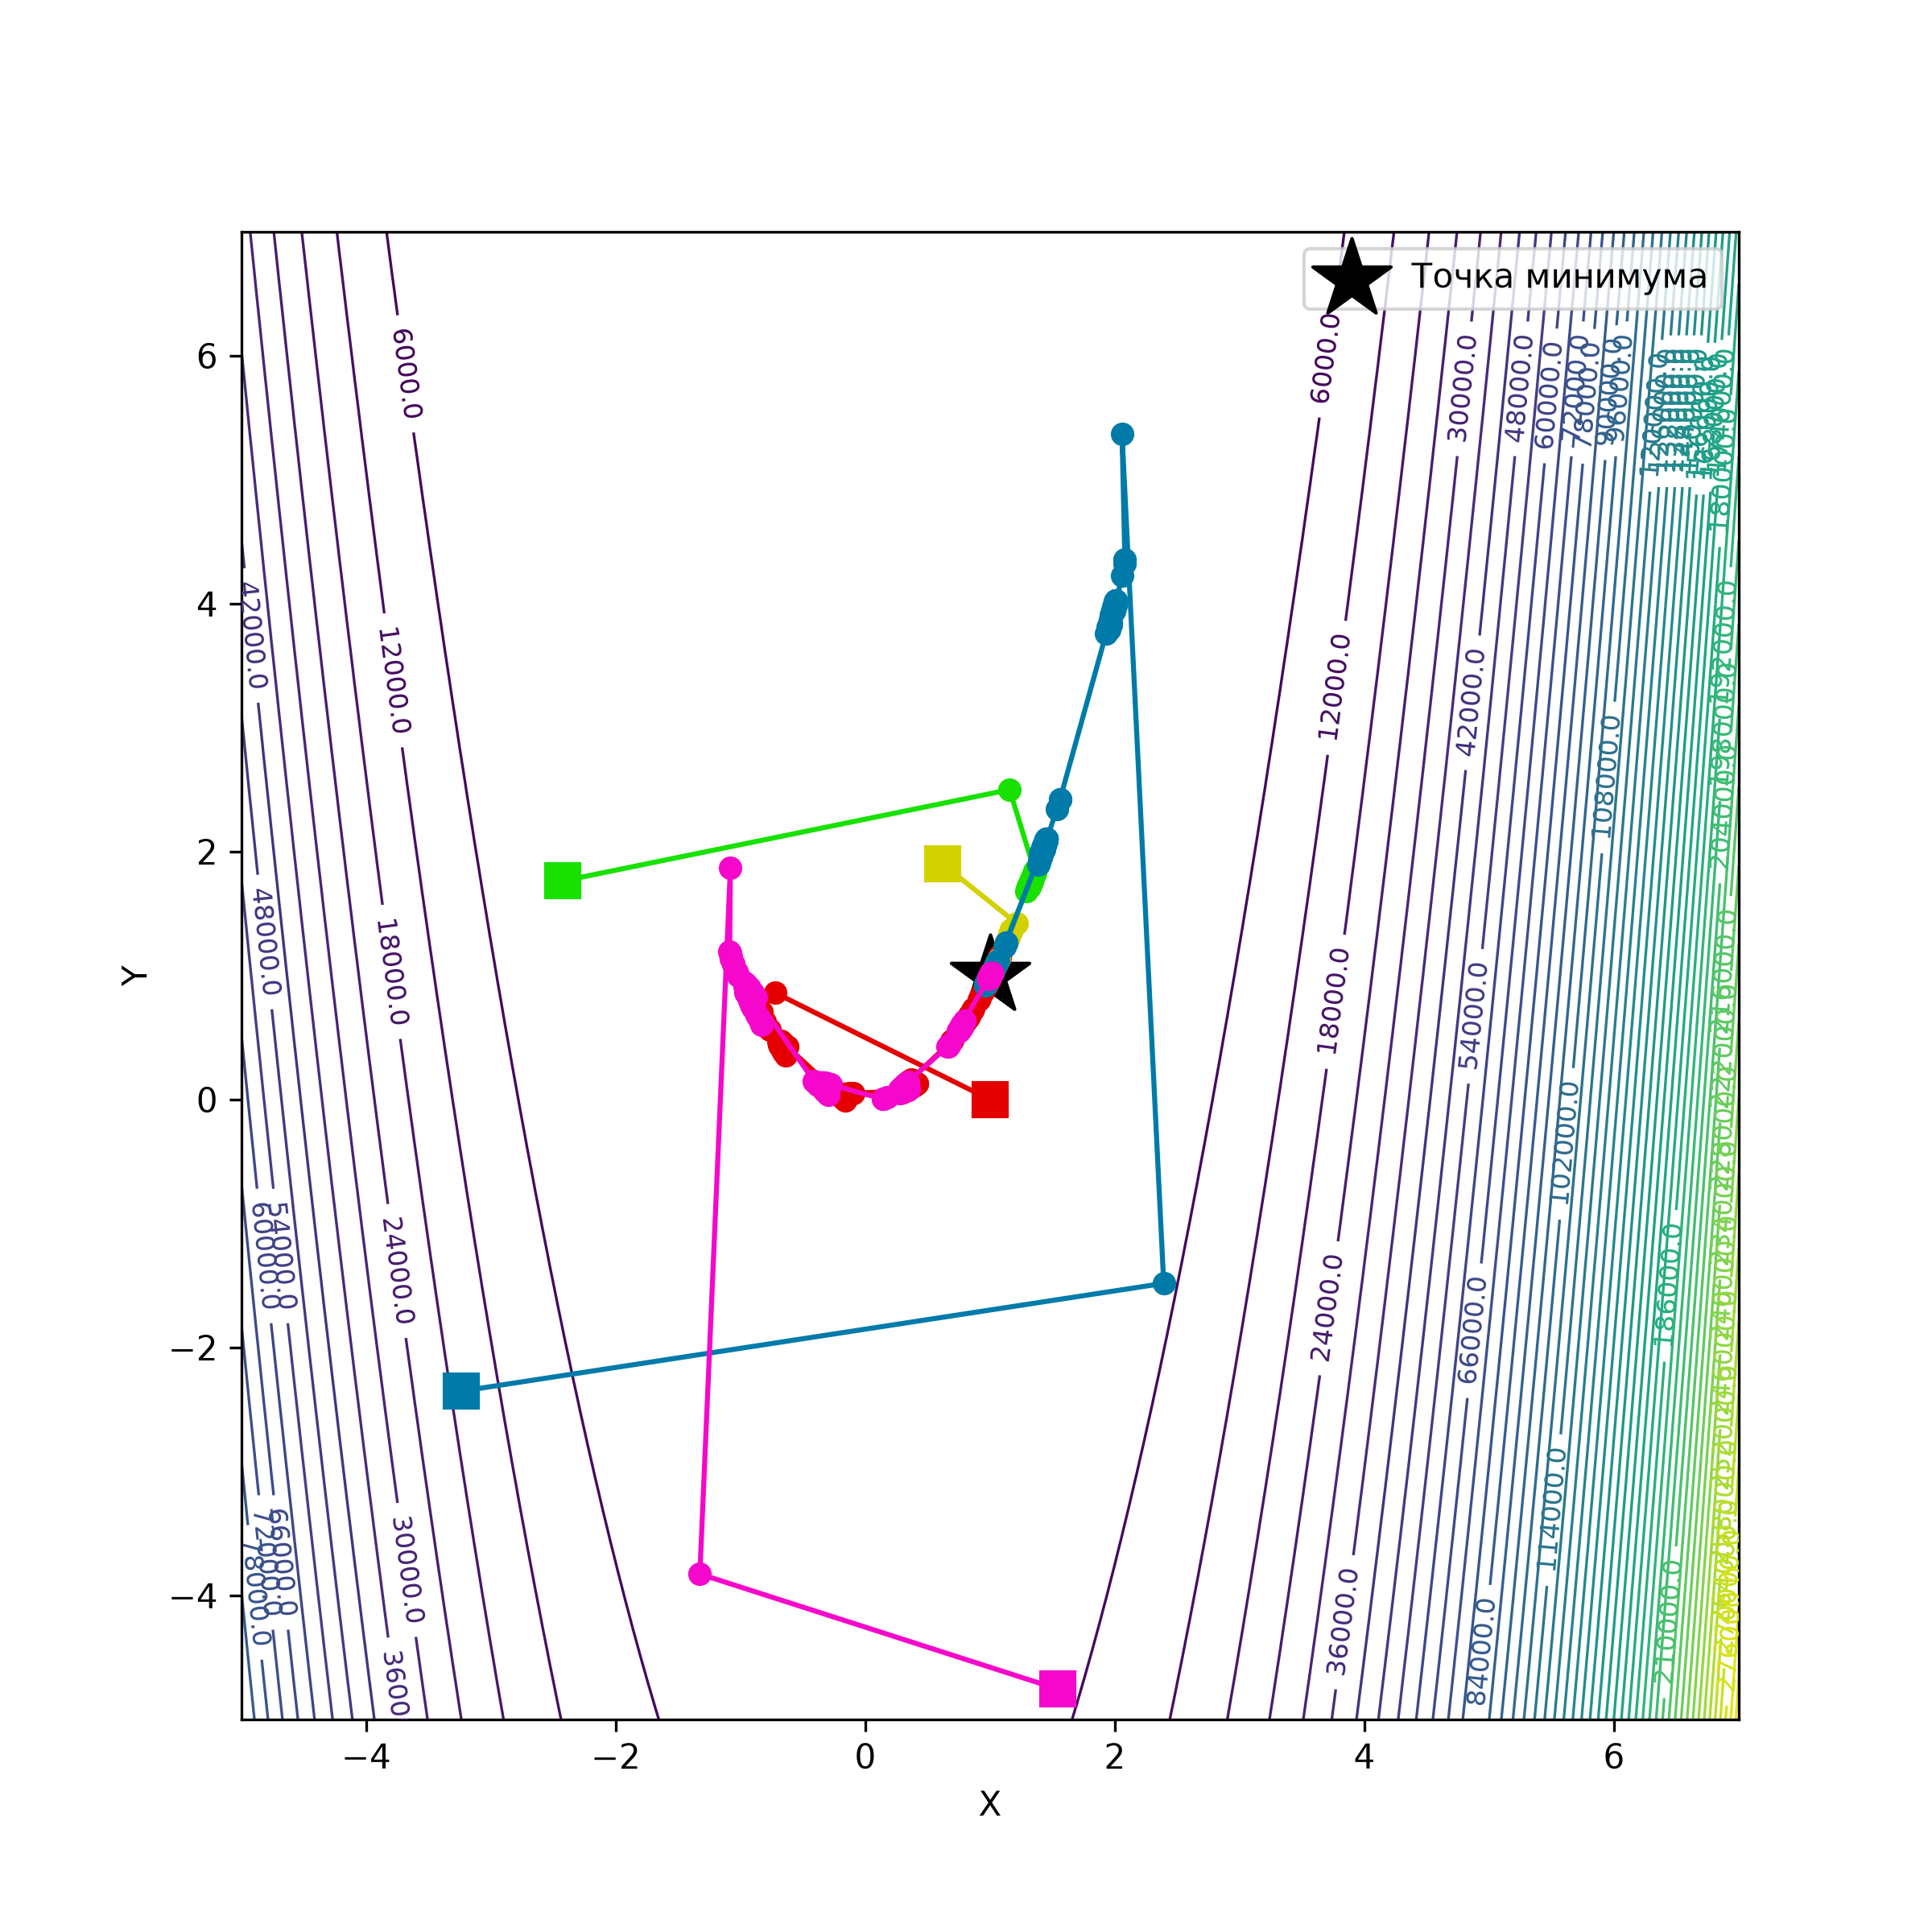
\includegraphics[width=0.3\textwidth]{task3_DFP_Rosenbrock function_plot.png}}%
\hfill % <-- Seperation
\subcaptionbox{BFGS}{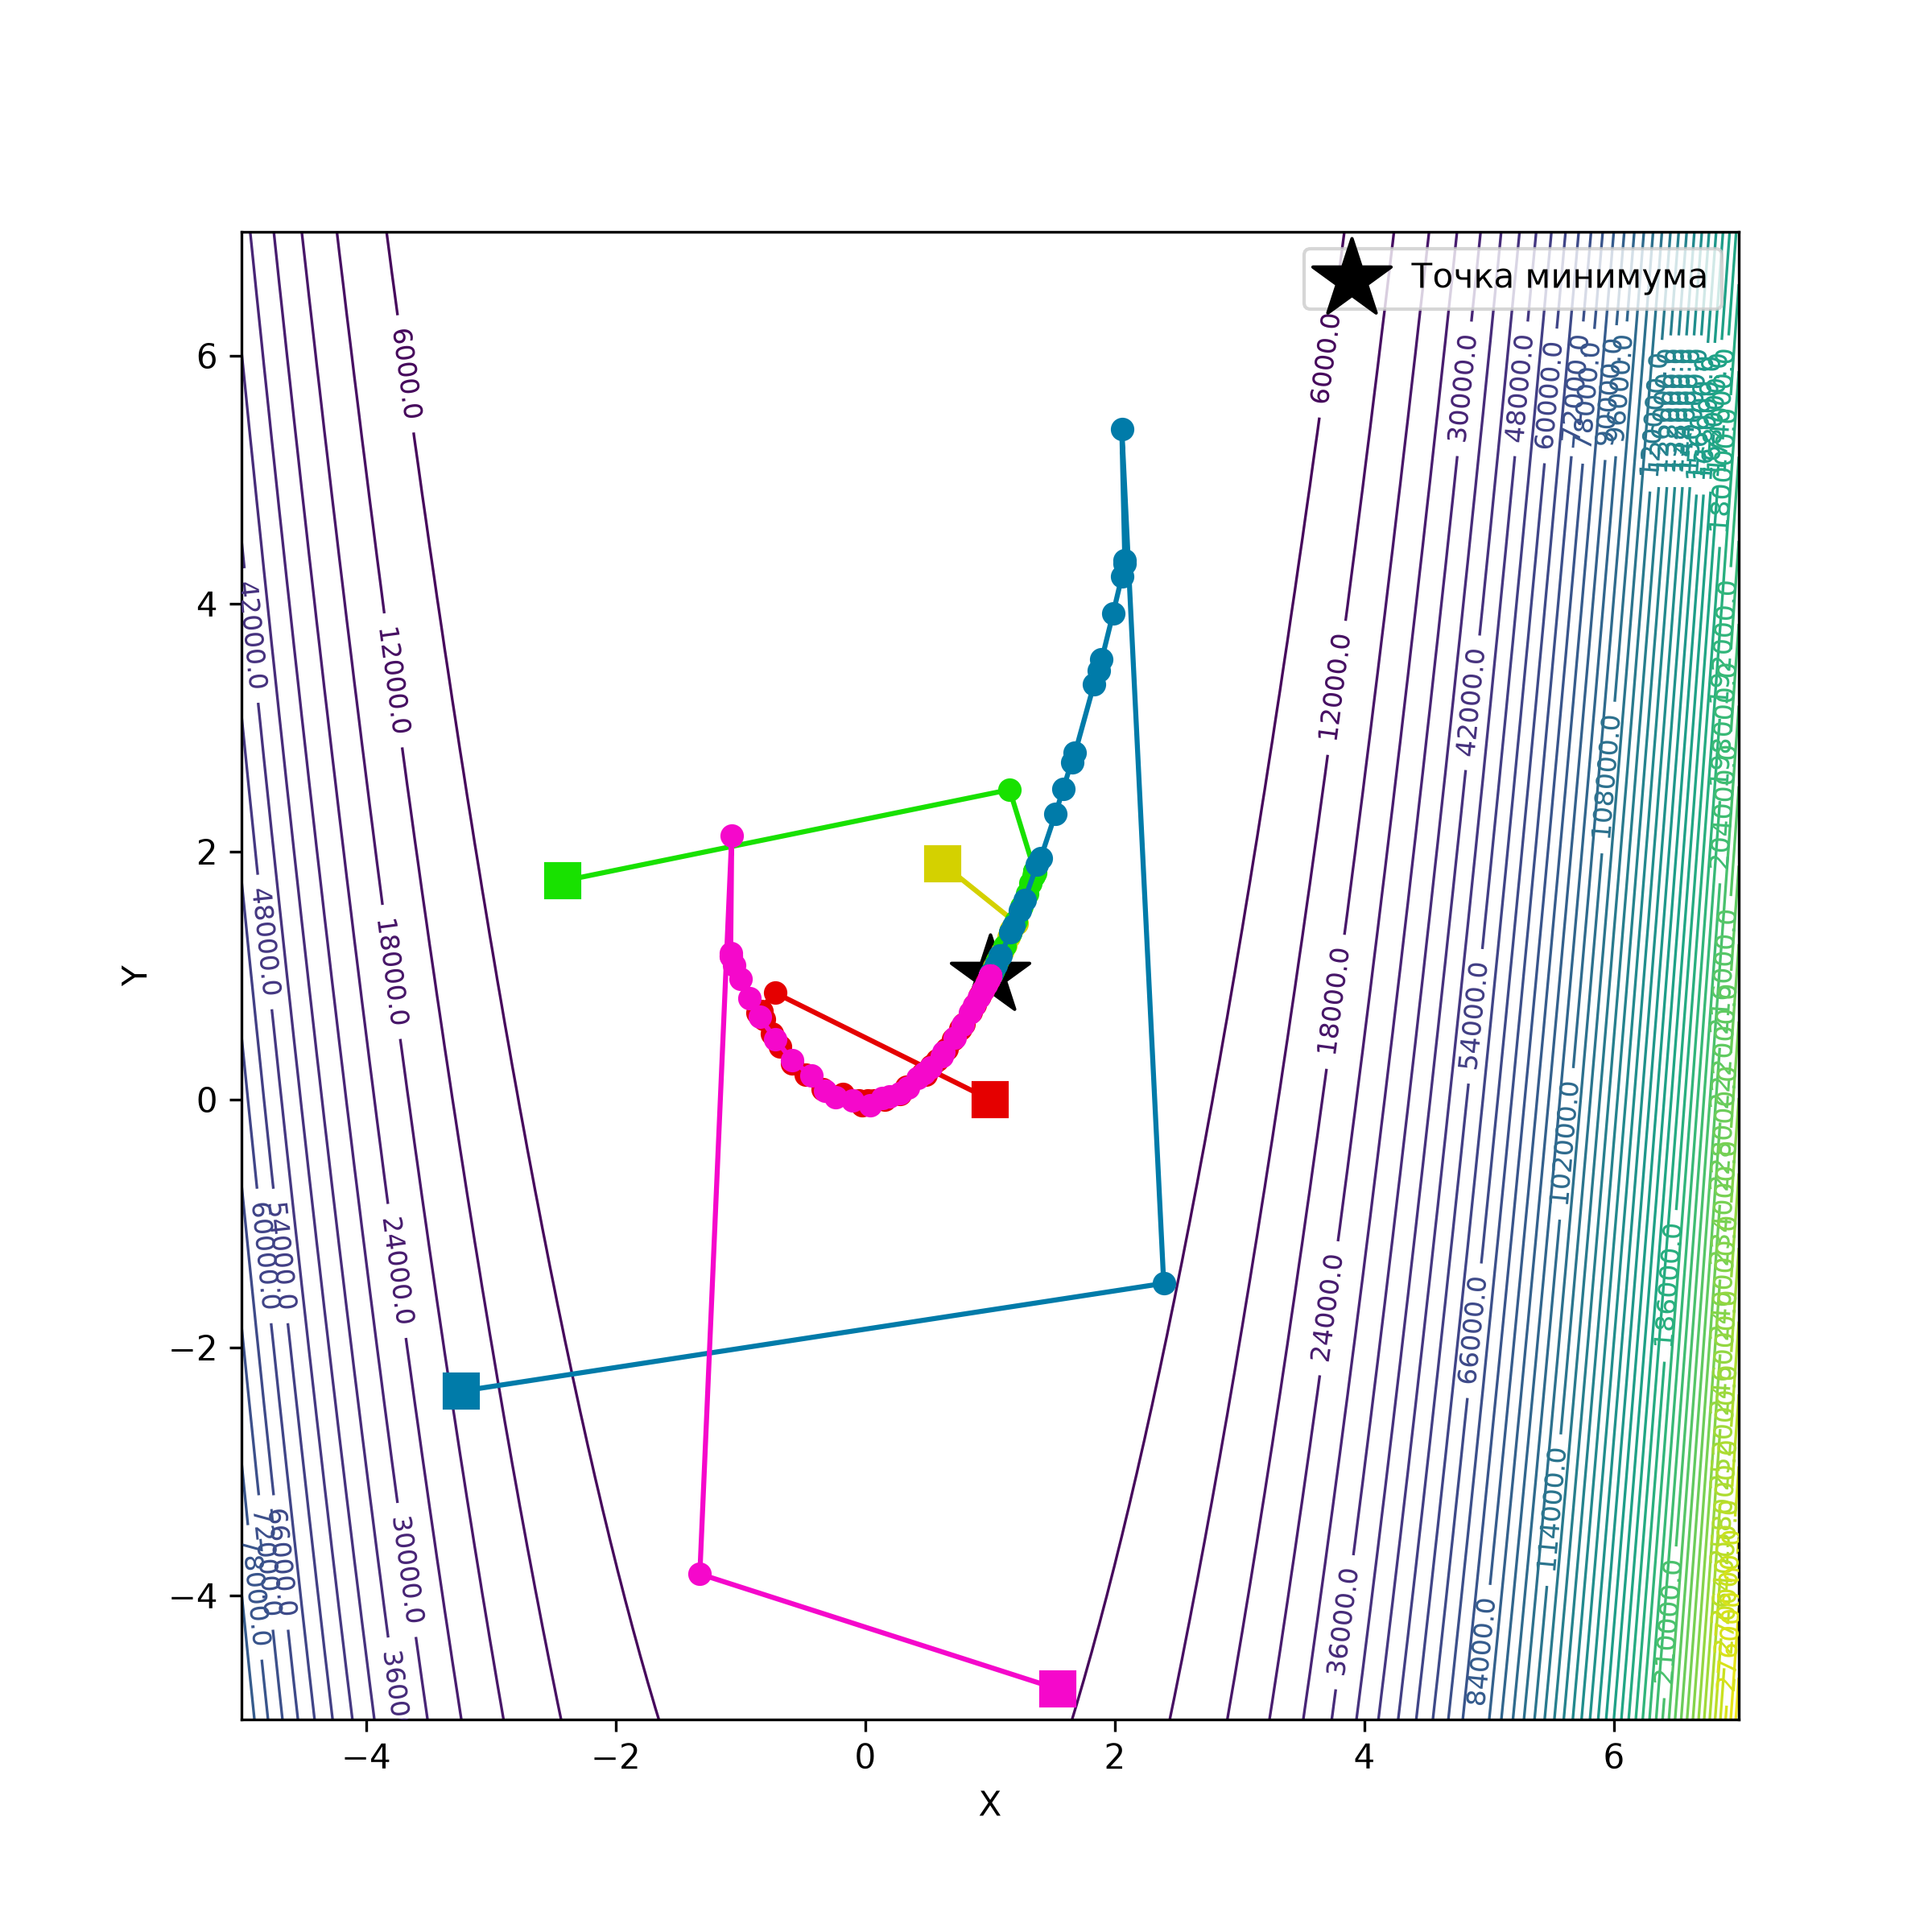
\includegraphics[width=0.3\textwidth]{task3_BFGS_Rosenbrock function_plot.png}}%
\hfill % <-- Seperation
\subcaptionbox{L-BFGS}{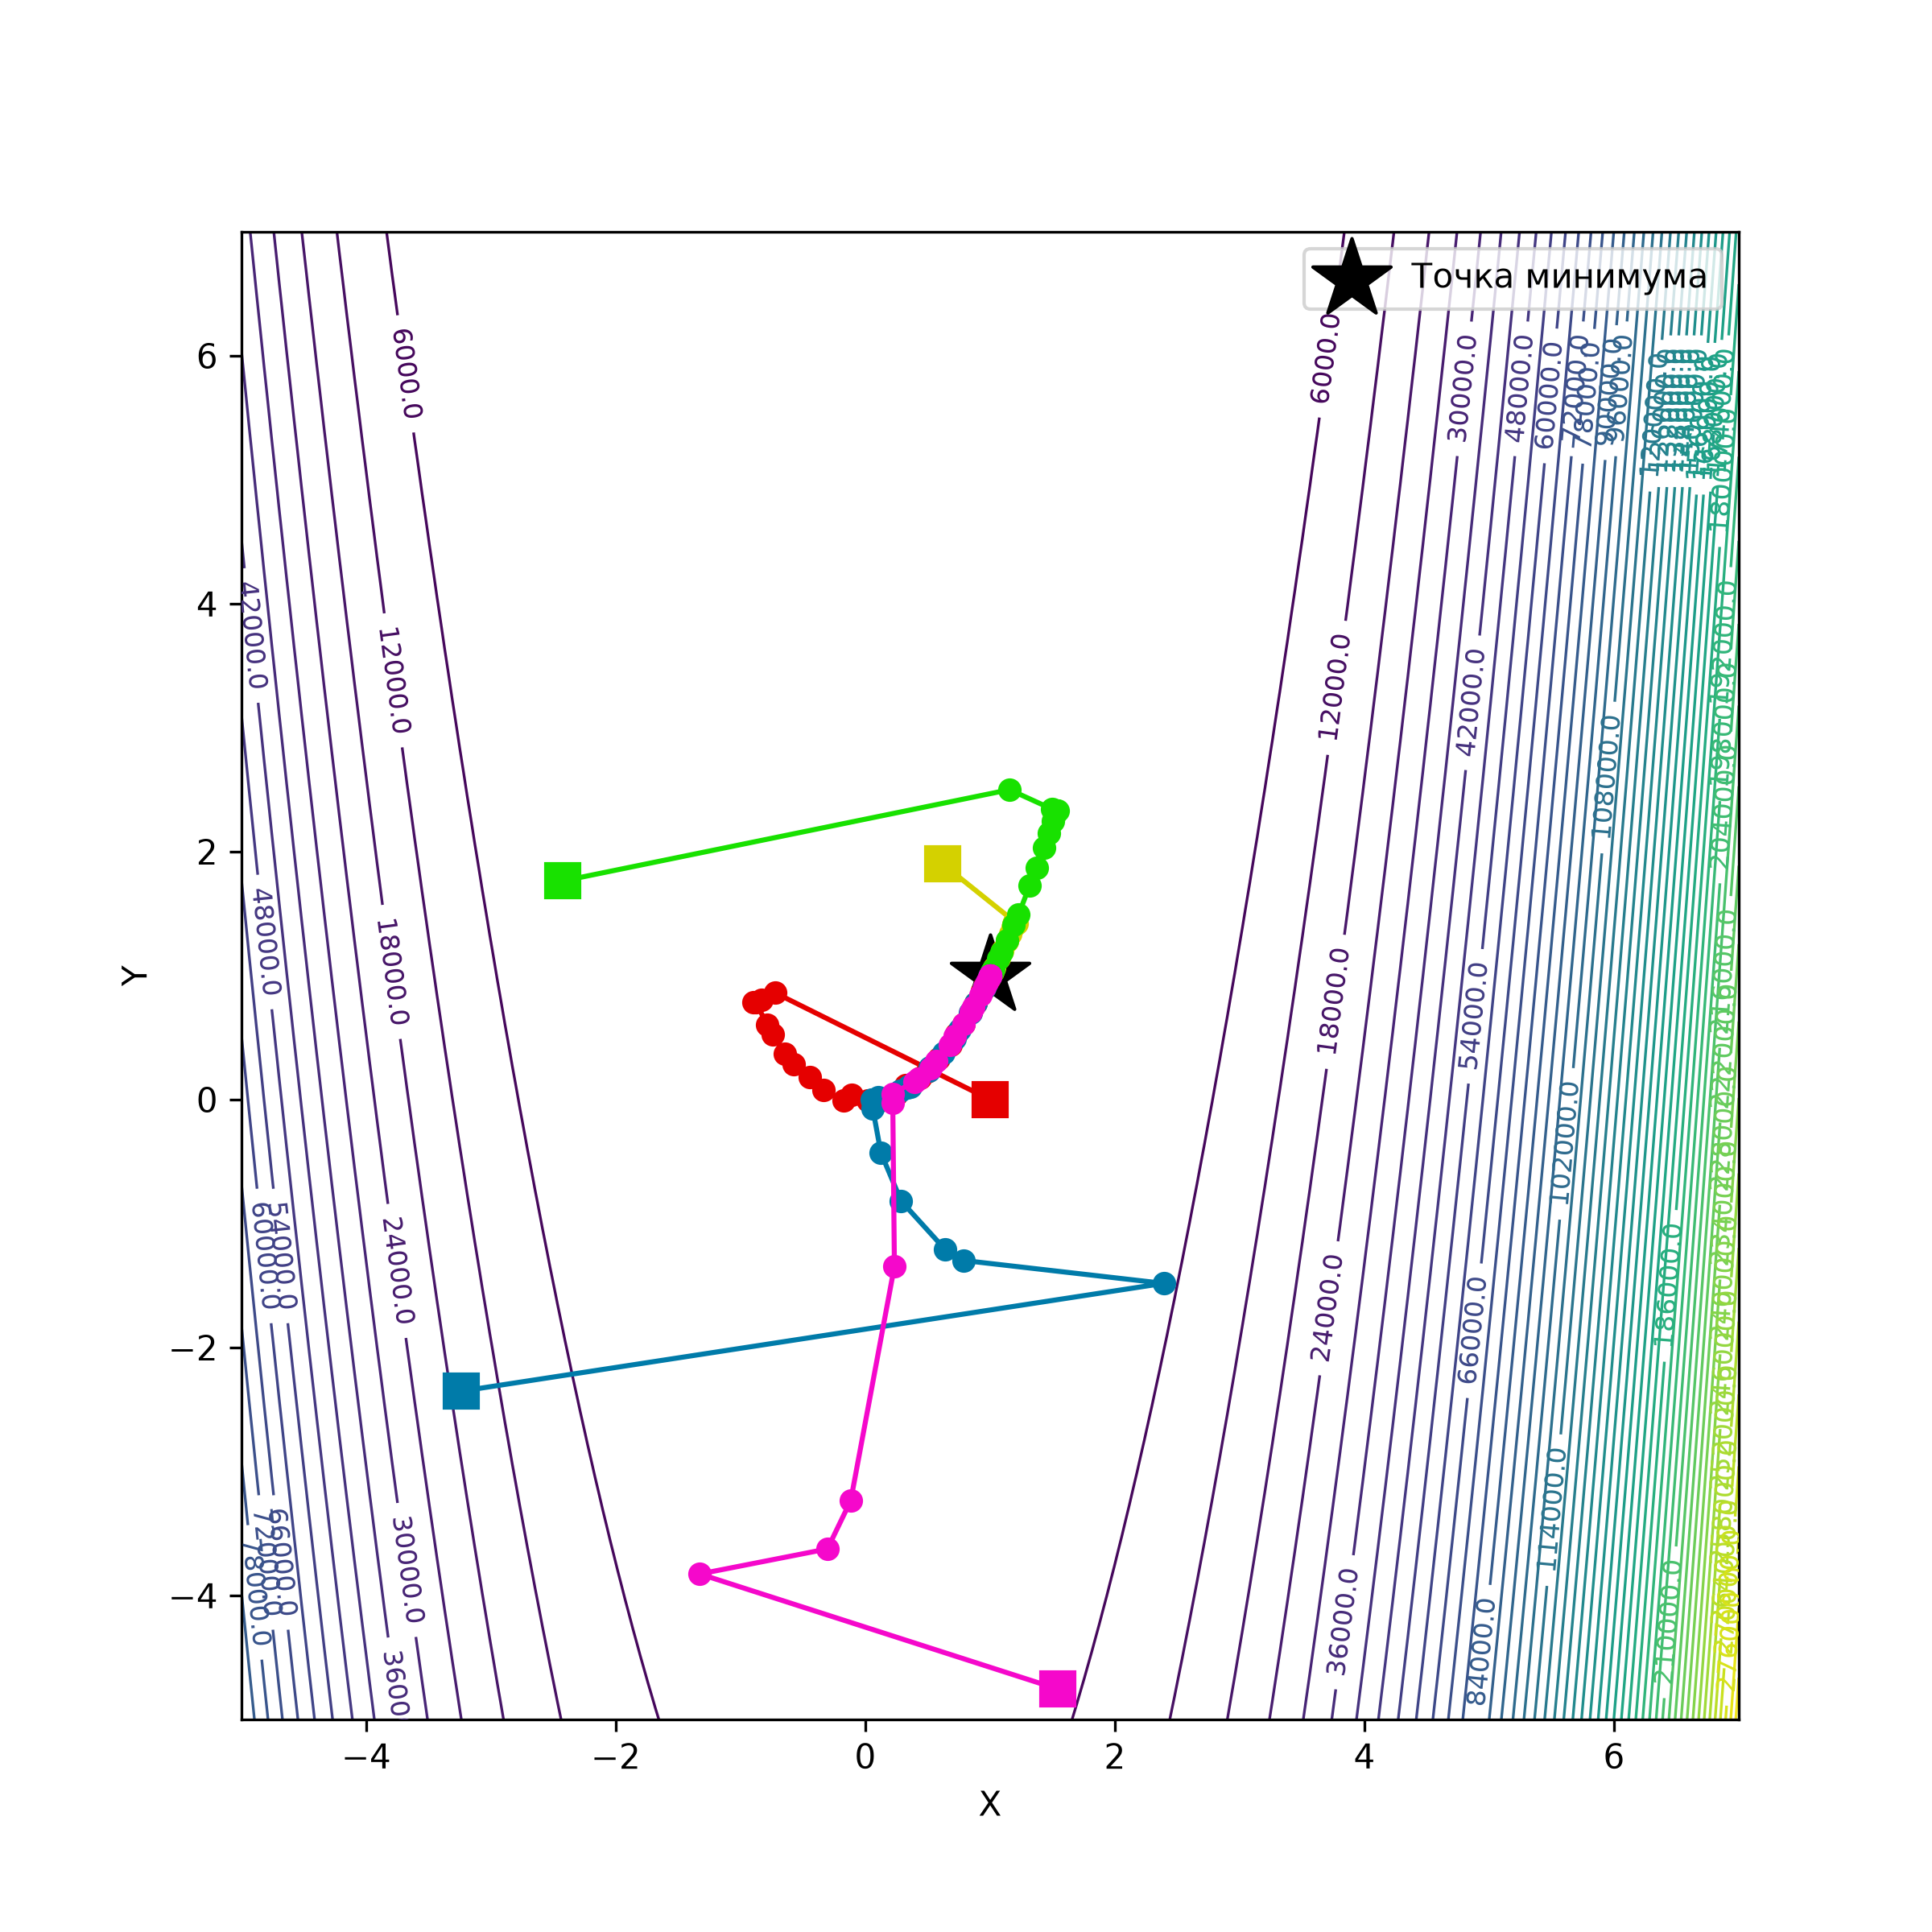
\includegraphics[width=0.3\textwidth]{task3_LBFGS_Rosenbrock function_plot.png}}%
\\ % <-- Line break
\caption{Работа оптимизаторов на функции Розенброка.}
\end{figure}

\begin{figure}[H]
\centering
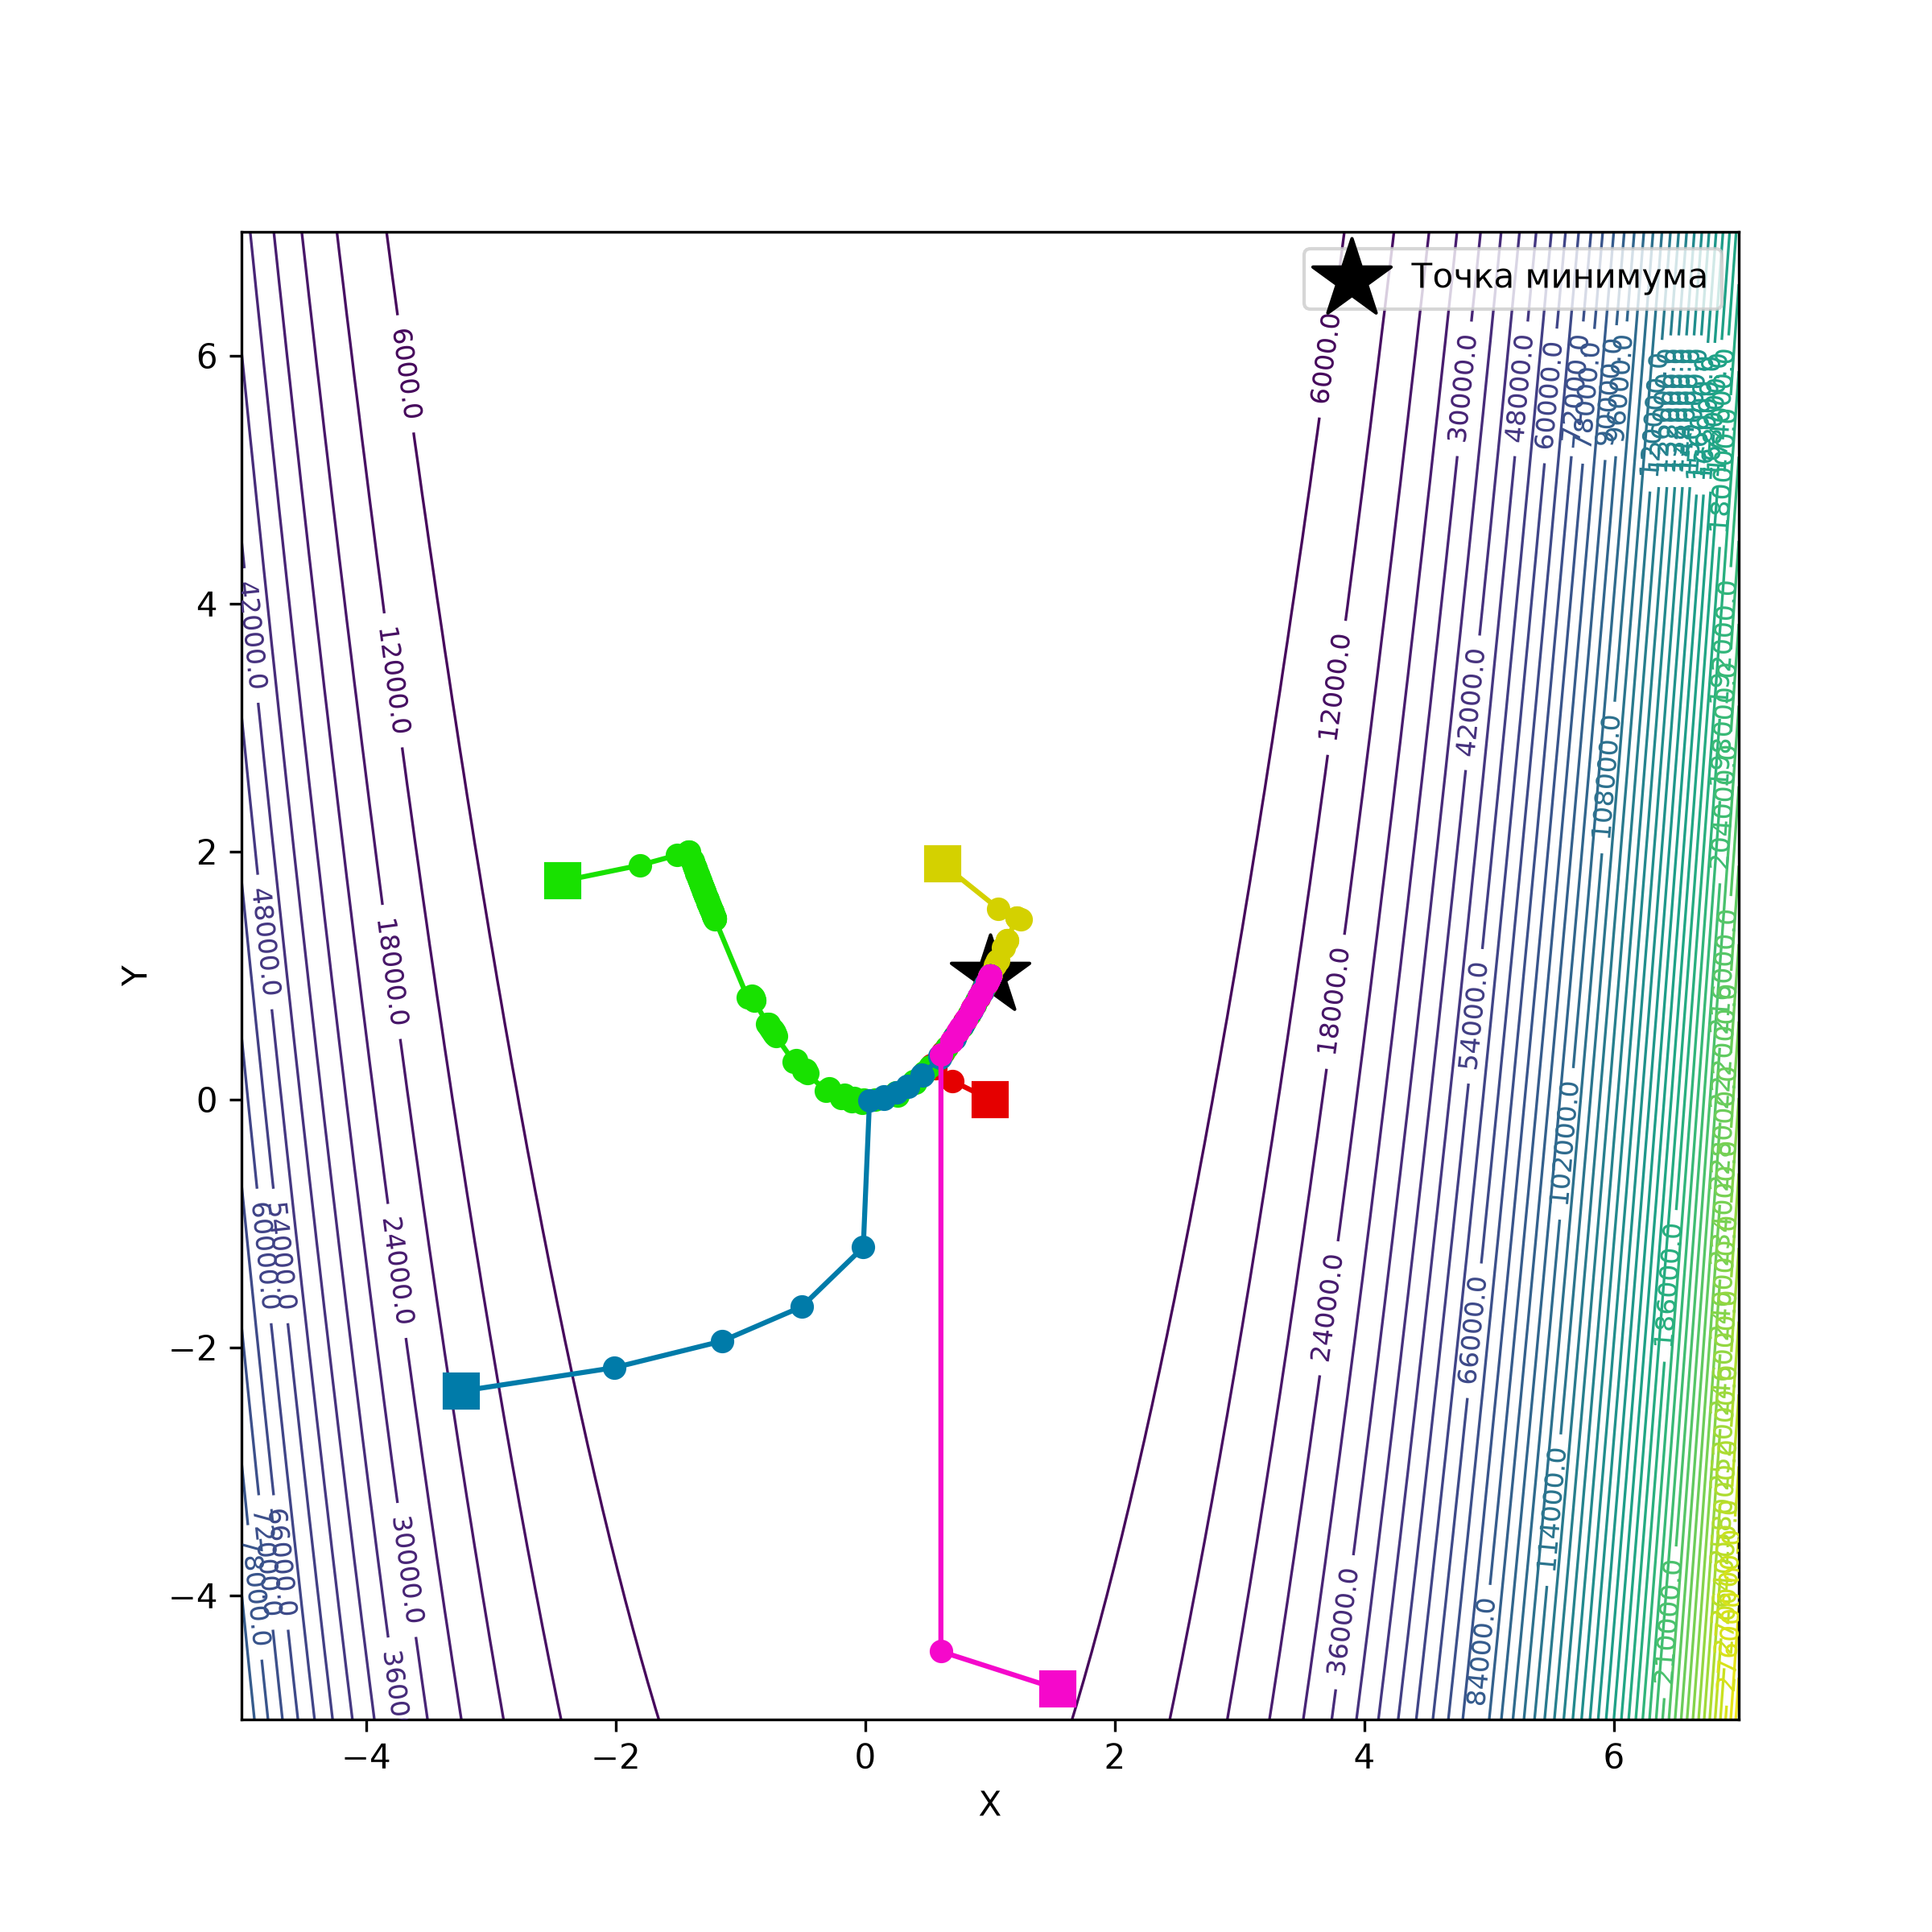
\includegraphics[width=1\textwidth]{task3_NewtonCG_Rosenbrock function_plot.png}
\caption{Работа библиотечной NewtonCG на функции Розенброка.}
\end{figure}

Видна численная нестабильность нелинейных методов сопряжённых градиентов, а также отсутствие сходимости линейного метода сопряжённых градиентов. Остальные методы спокойно сходятся к точке минимума

Также следует обратить внимание на метод Ньютона с разложением Холецкого: при старте из жёлтой точки с координатами (0.618,1.902) метод даже не начинает поиск, заканчиваясь с ошибкой на первой же итерации. Это вызвано тем, что в данной точке матрица не положительно определённая, вследствие чего алгоритм вынужден остановить работу.

Также обратим внимание на особенность движение методов у \enquote{оврага}: они не совершают зигзагобразных колебаний возле него; вместо этого они перемещаются вдоль оврага, что более оптимально.

Сравнивая с библиотечным NewtonCG, видно, что данный метод лучше справляется с задачей, чем все остальные методы.

\begin{figure}[H]
\centering
\subcaptionbox{Сопр. градиенты}{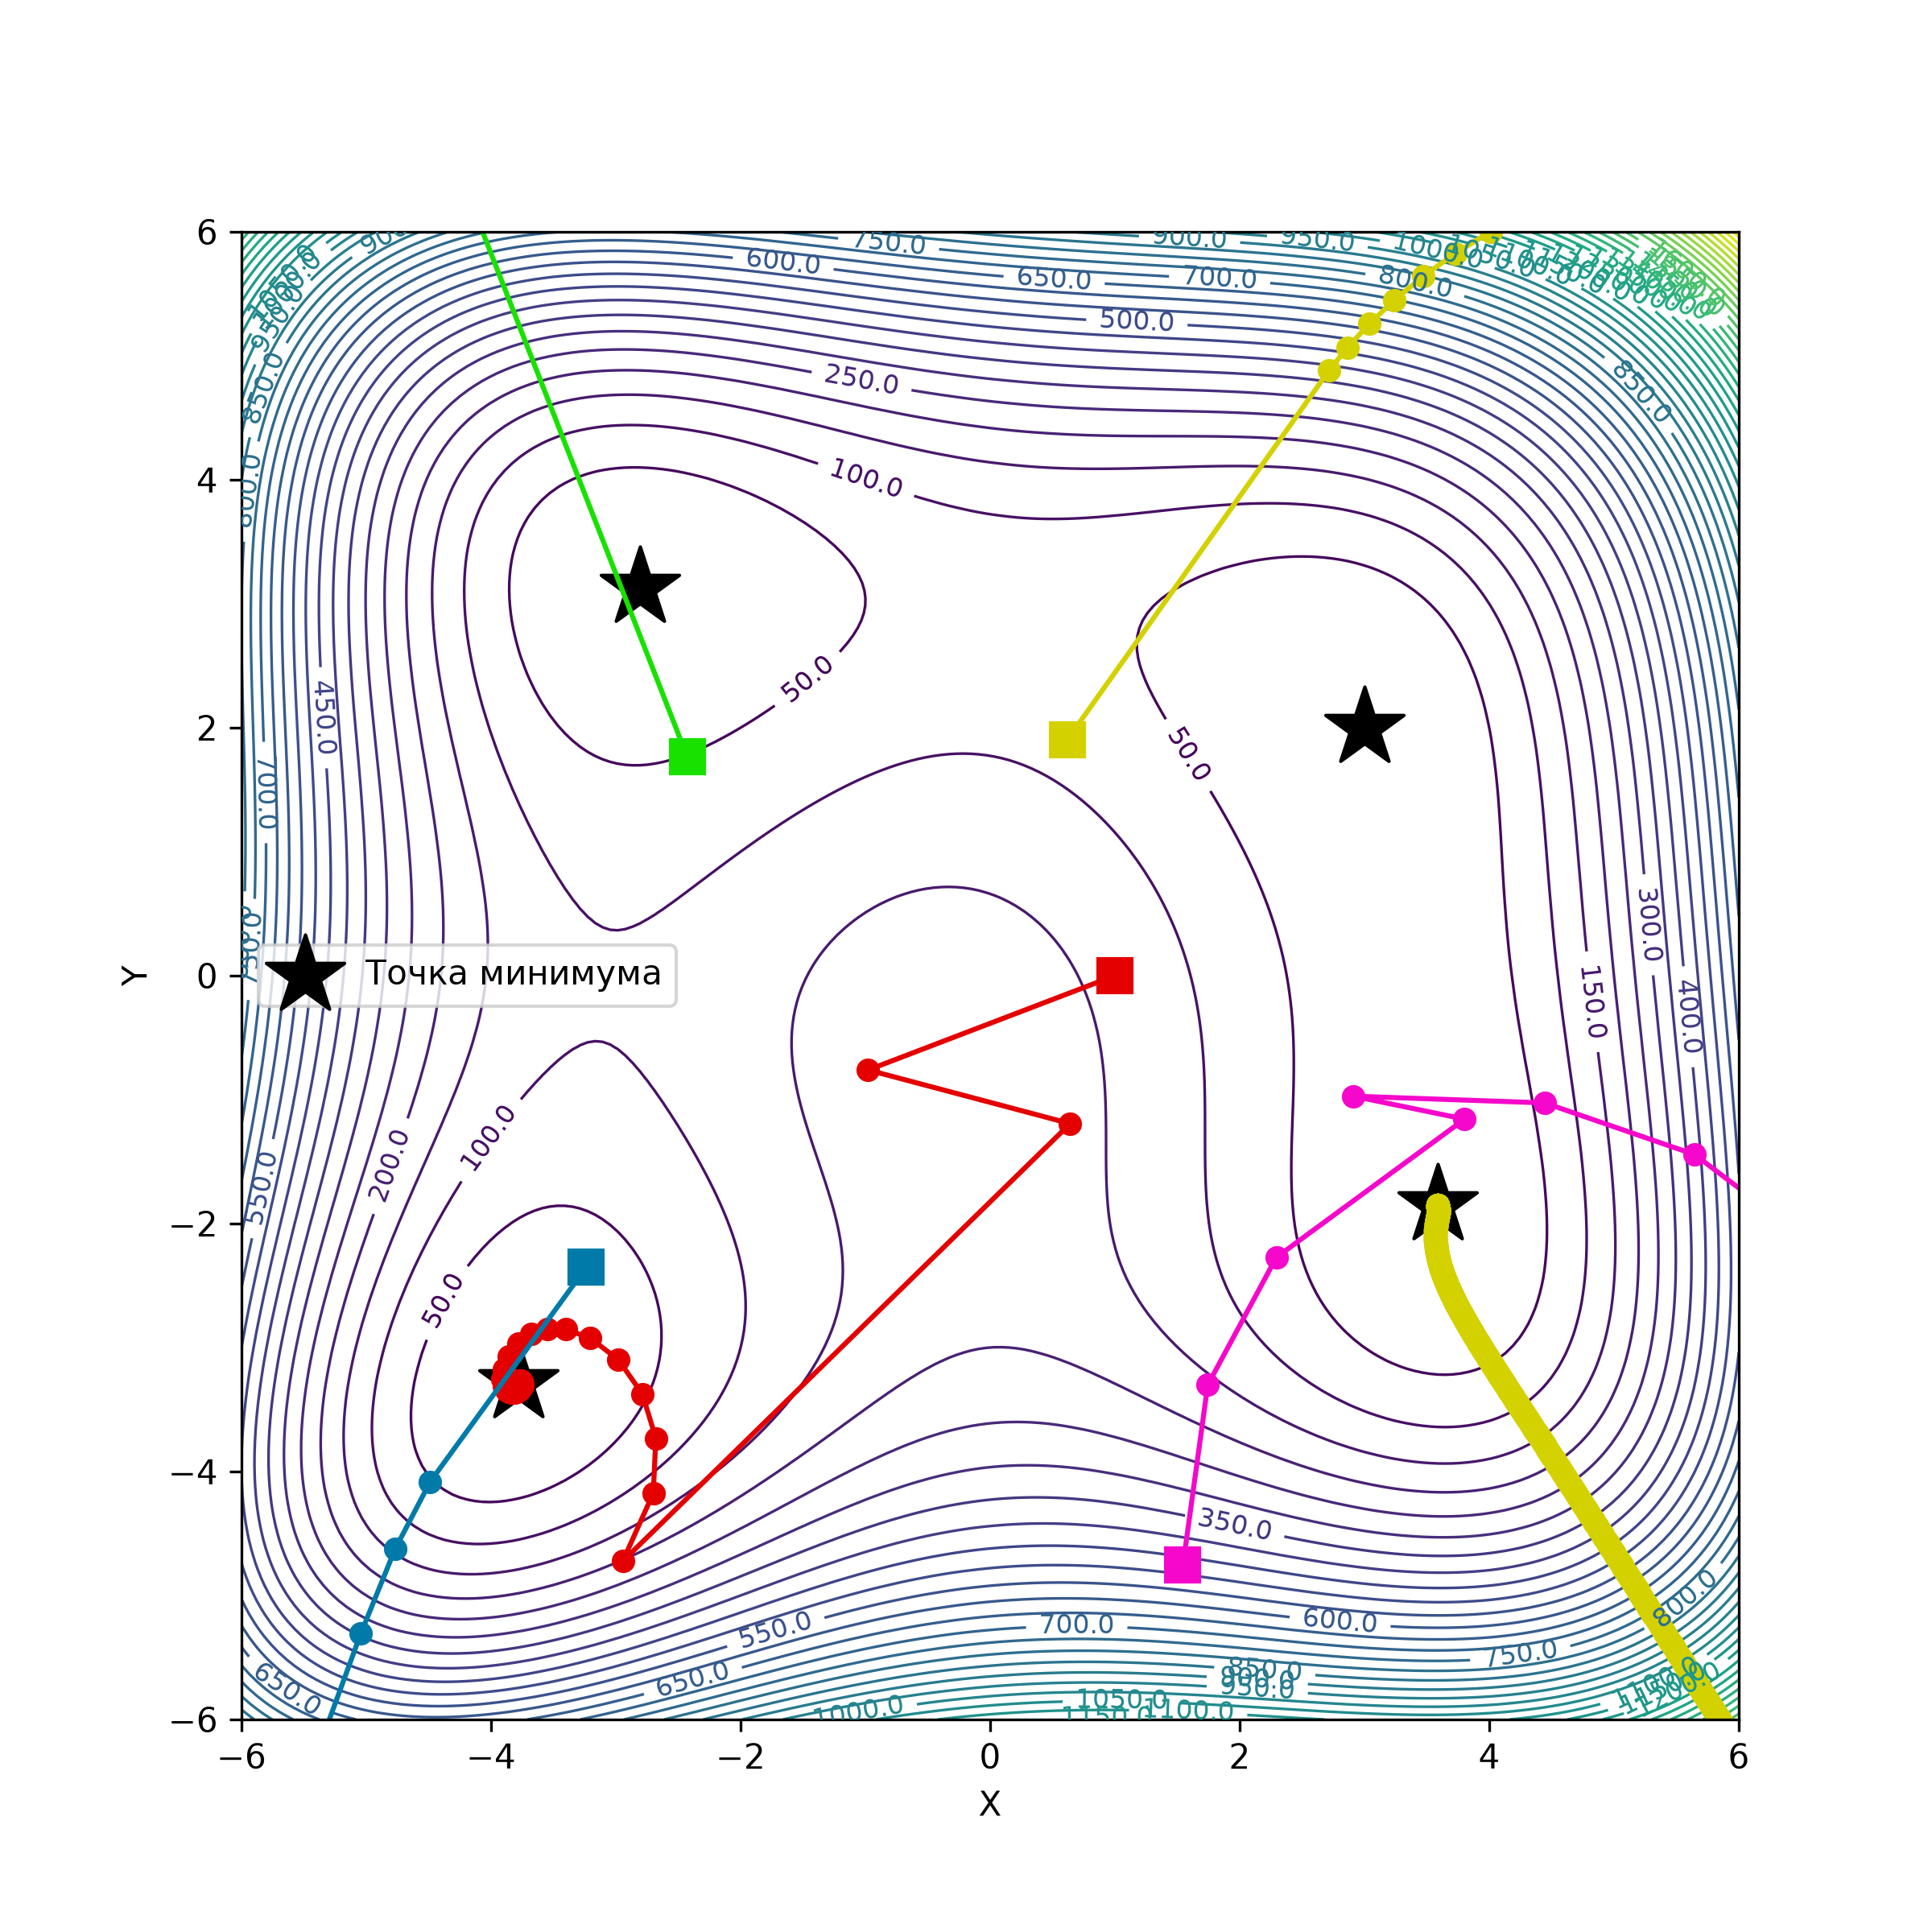
\includegraphics[width=0.3\textwidth]{task3_LinearConjugateGradient_Himmelblau function_plot.png}}%
\hfill % <-- Seperation
\subcaptionbox{Флетчер-Ривс}{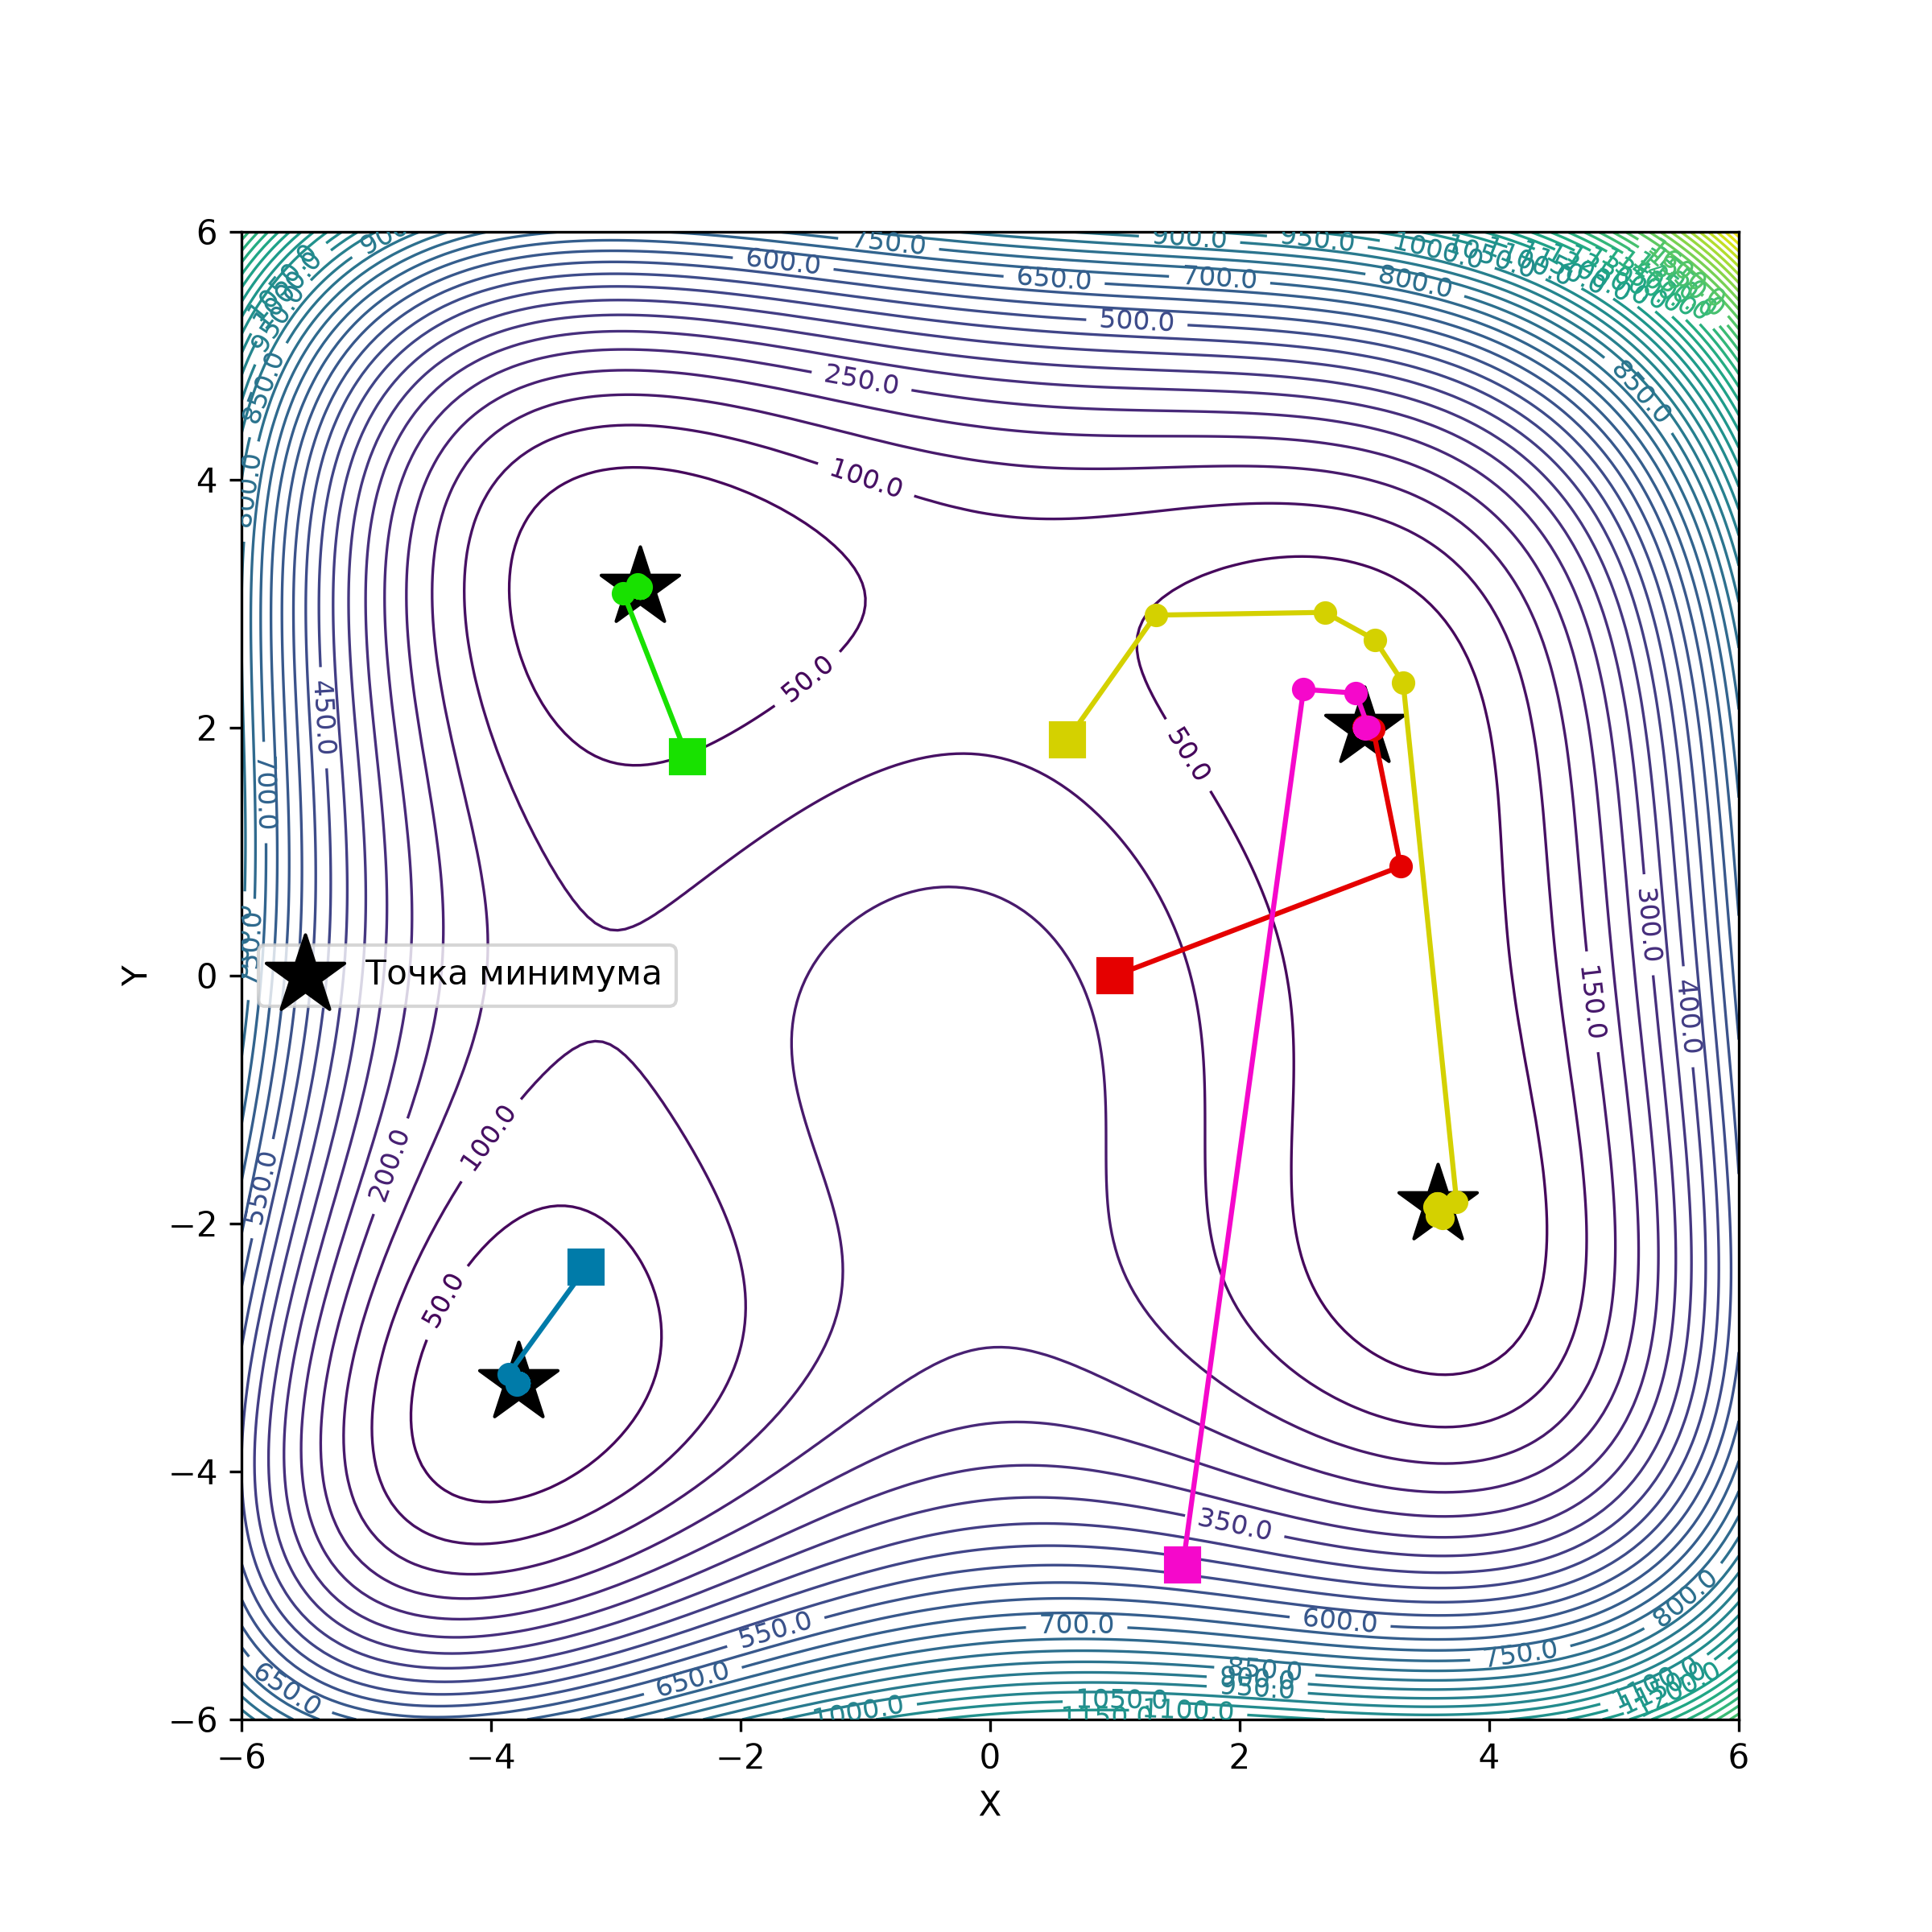
\includegraphics[width=0.3\textwidth]{task3_FletcherReeves_Himmelblau function_plot.png}}%
\hfill % <-- Seperation
\subcaptionbox{Полак-Рибьер}{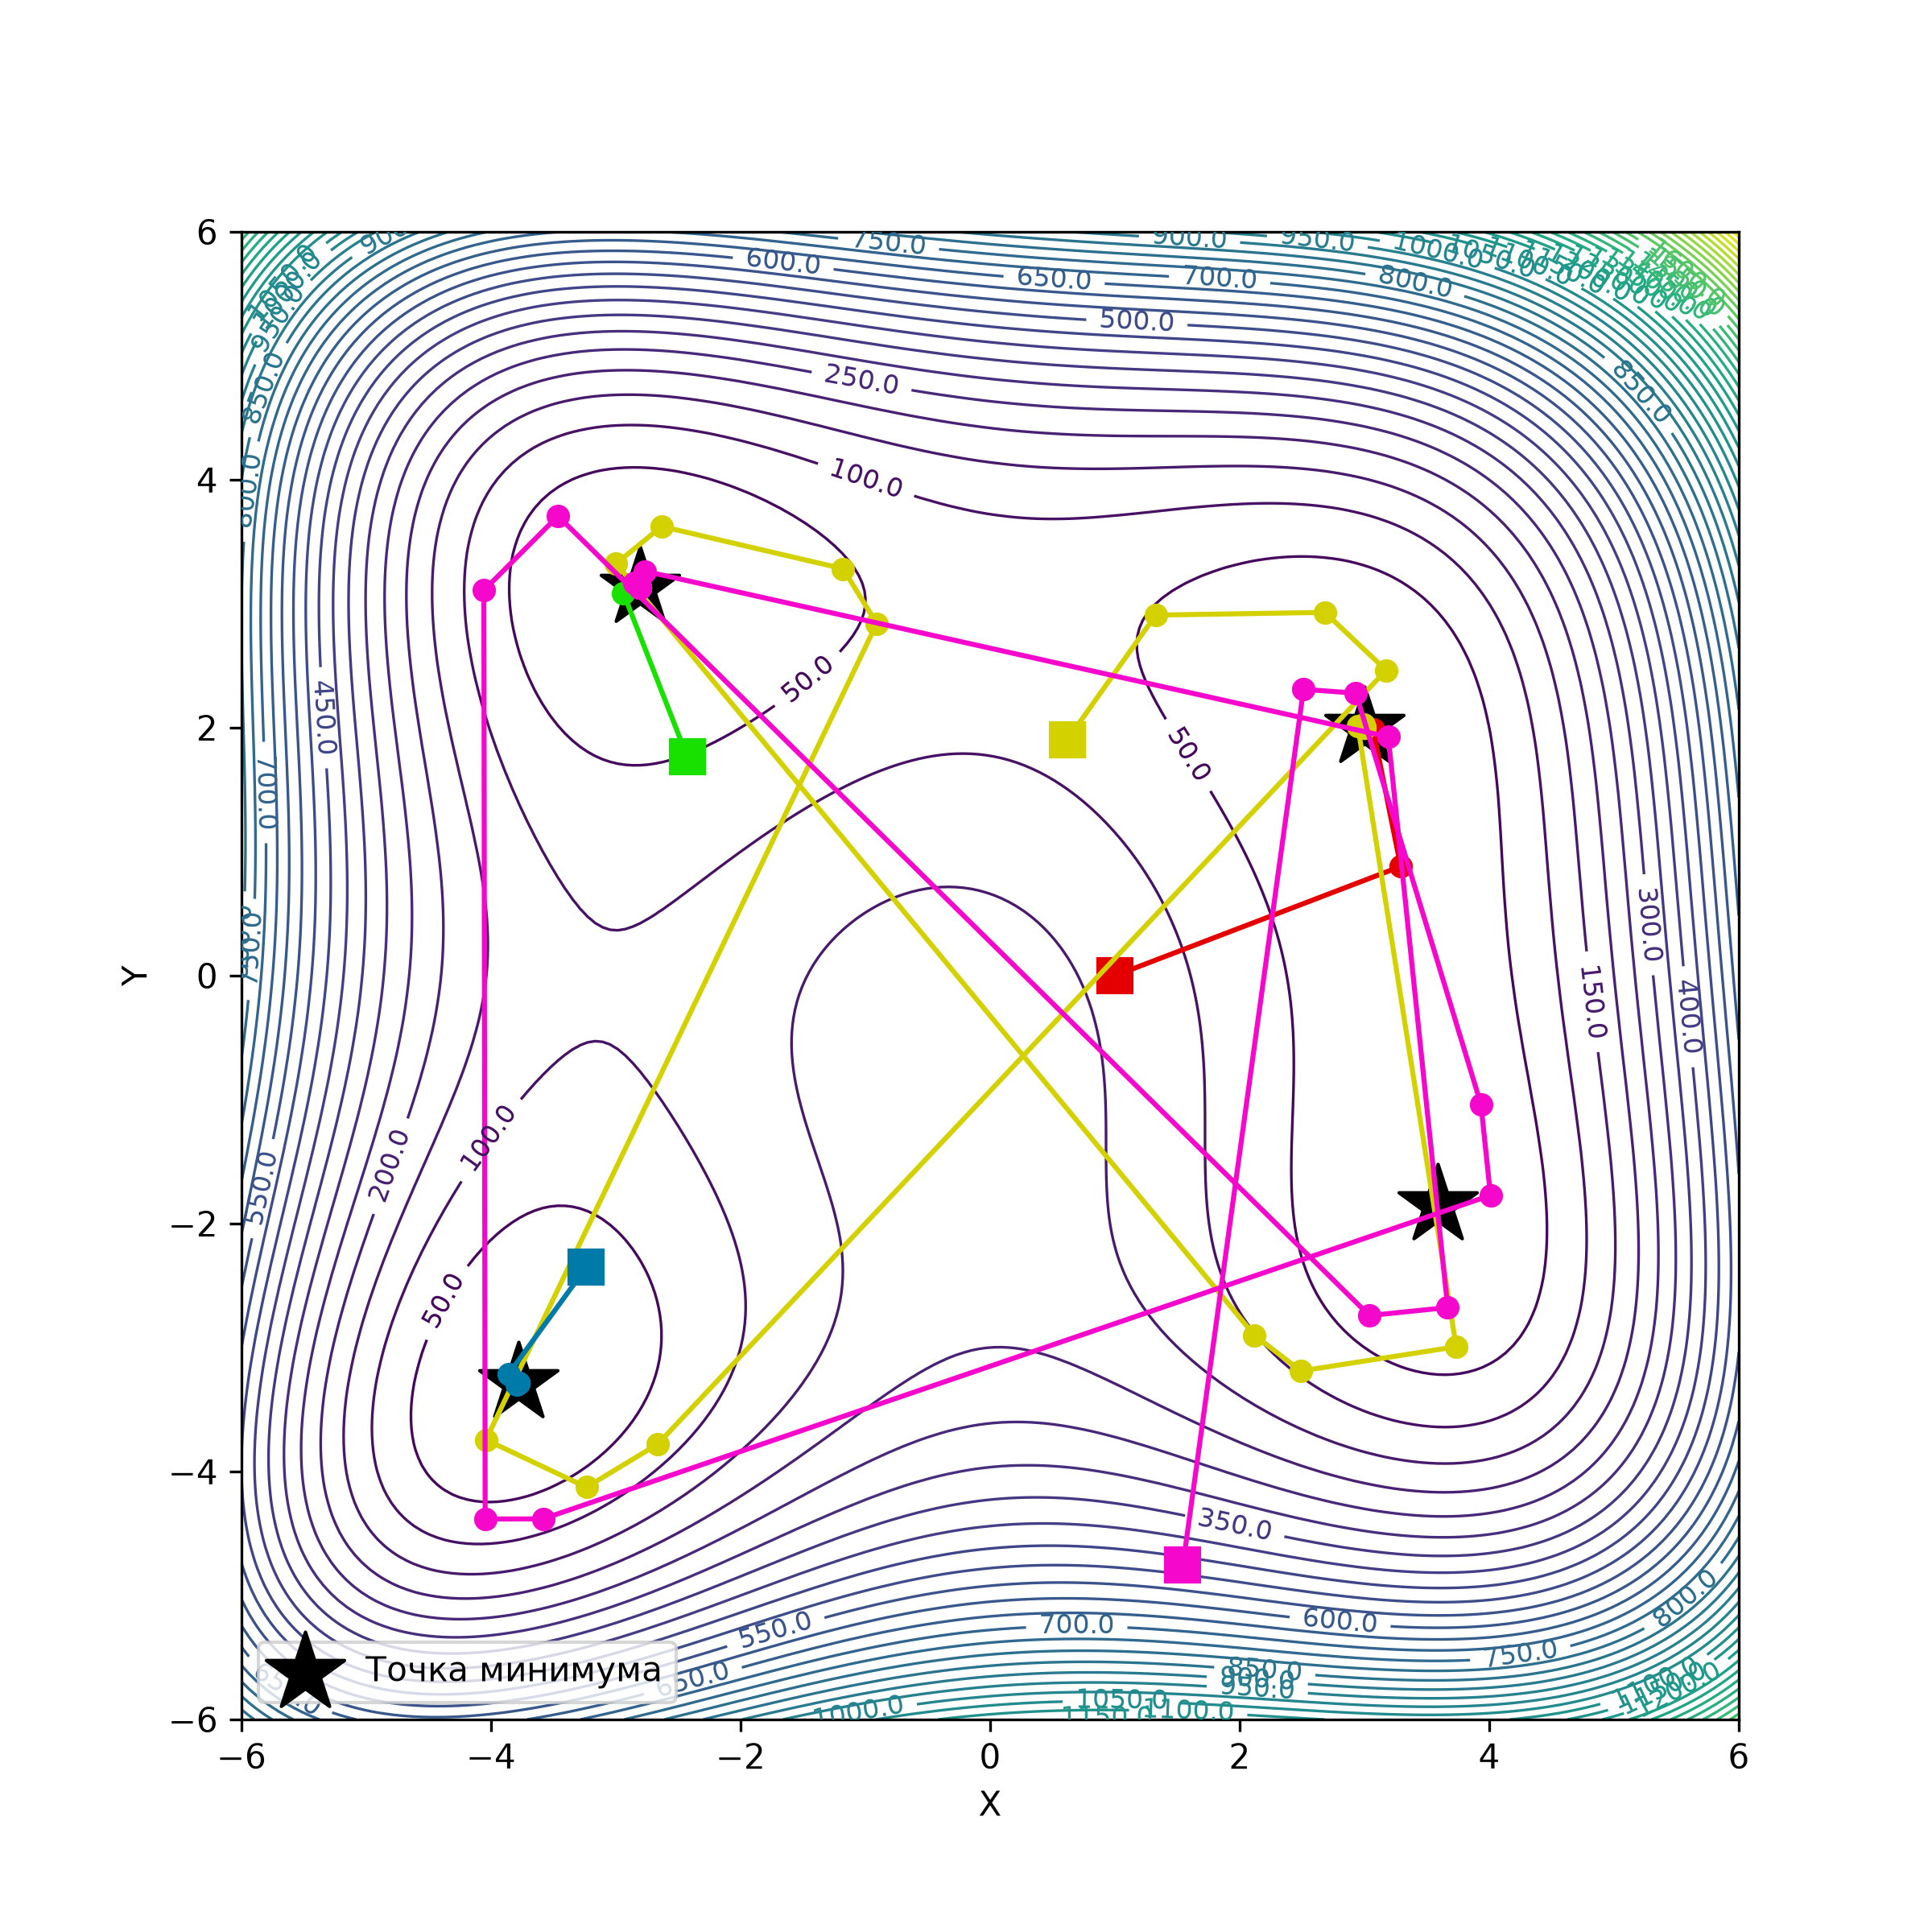
\includegraphics[width=0.3\textwidth]{task3_PolakRibiere_Himmelblau function_plot.png}}%
\\ % <-- Line break
\centering
\subcaptionbox{Разл. Холецкого}{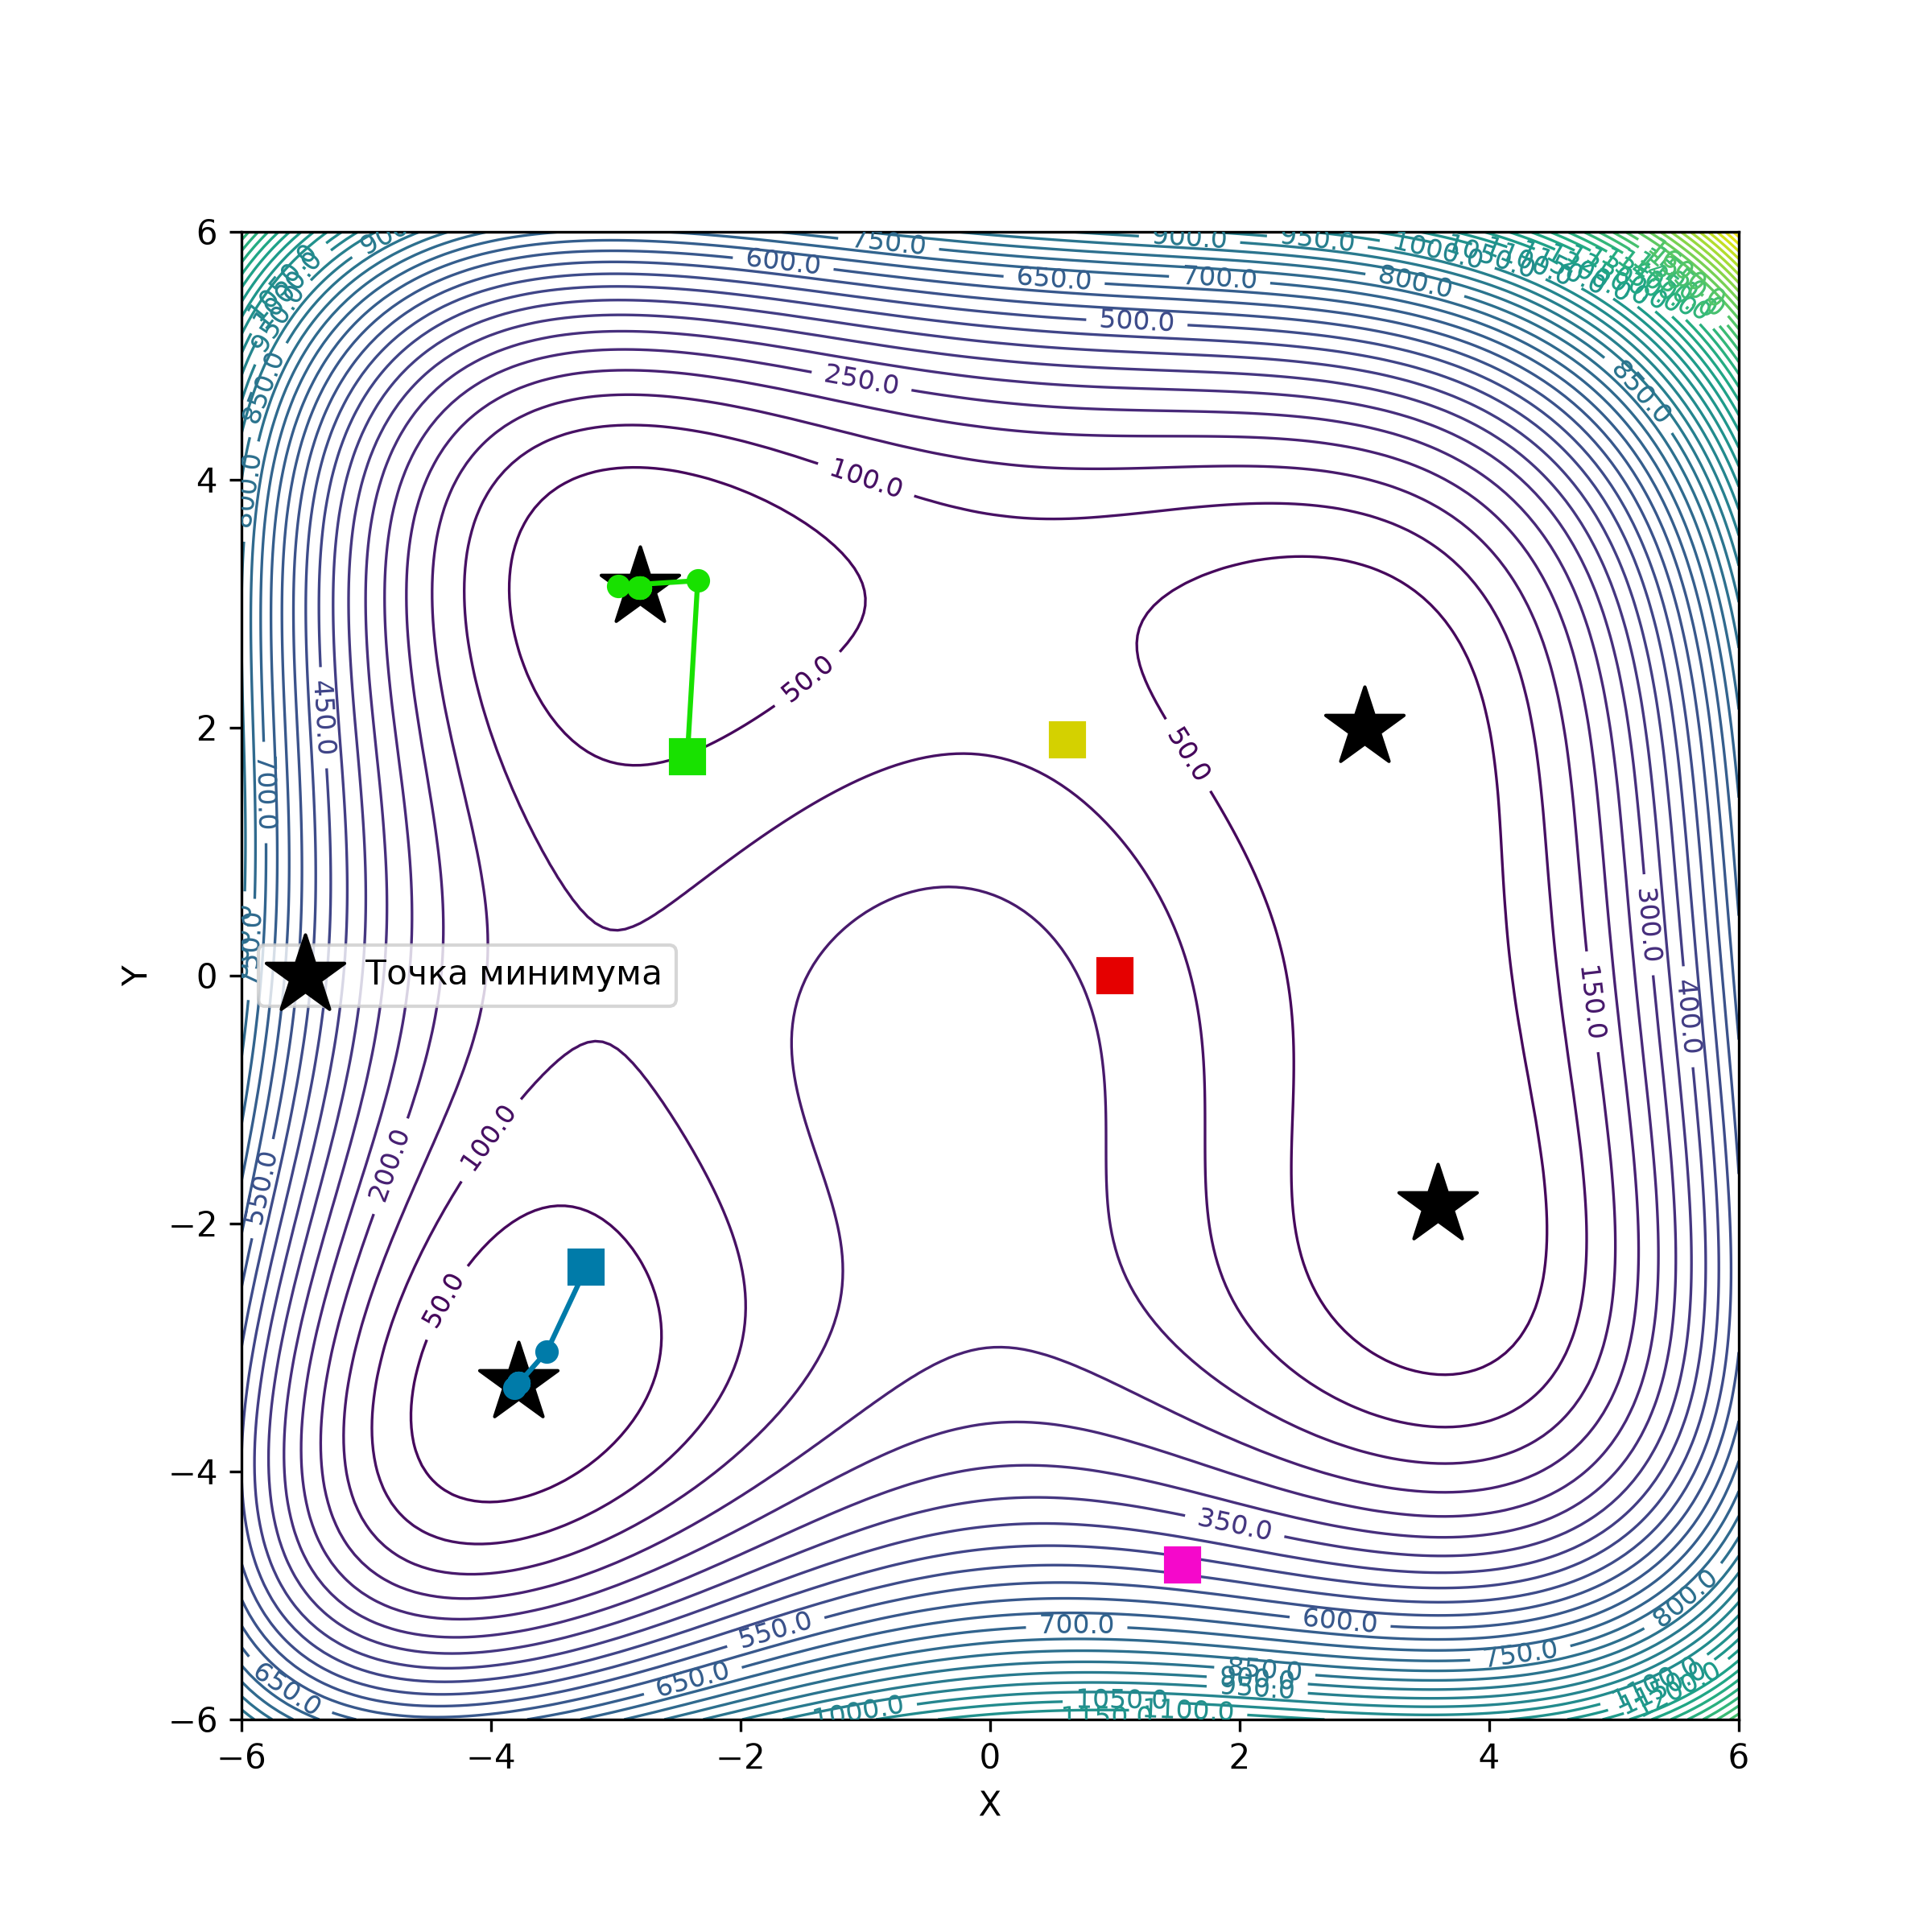
\includegraphics[width=0.3\textwidth]{task3_NewtonCholesky_Himmelblau function_plot.png}}%
\hfill % <-- Seperation
\subcaptionbox{Выбор направления}{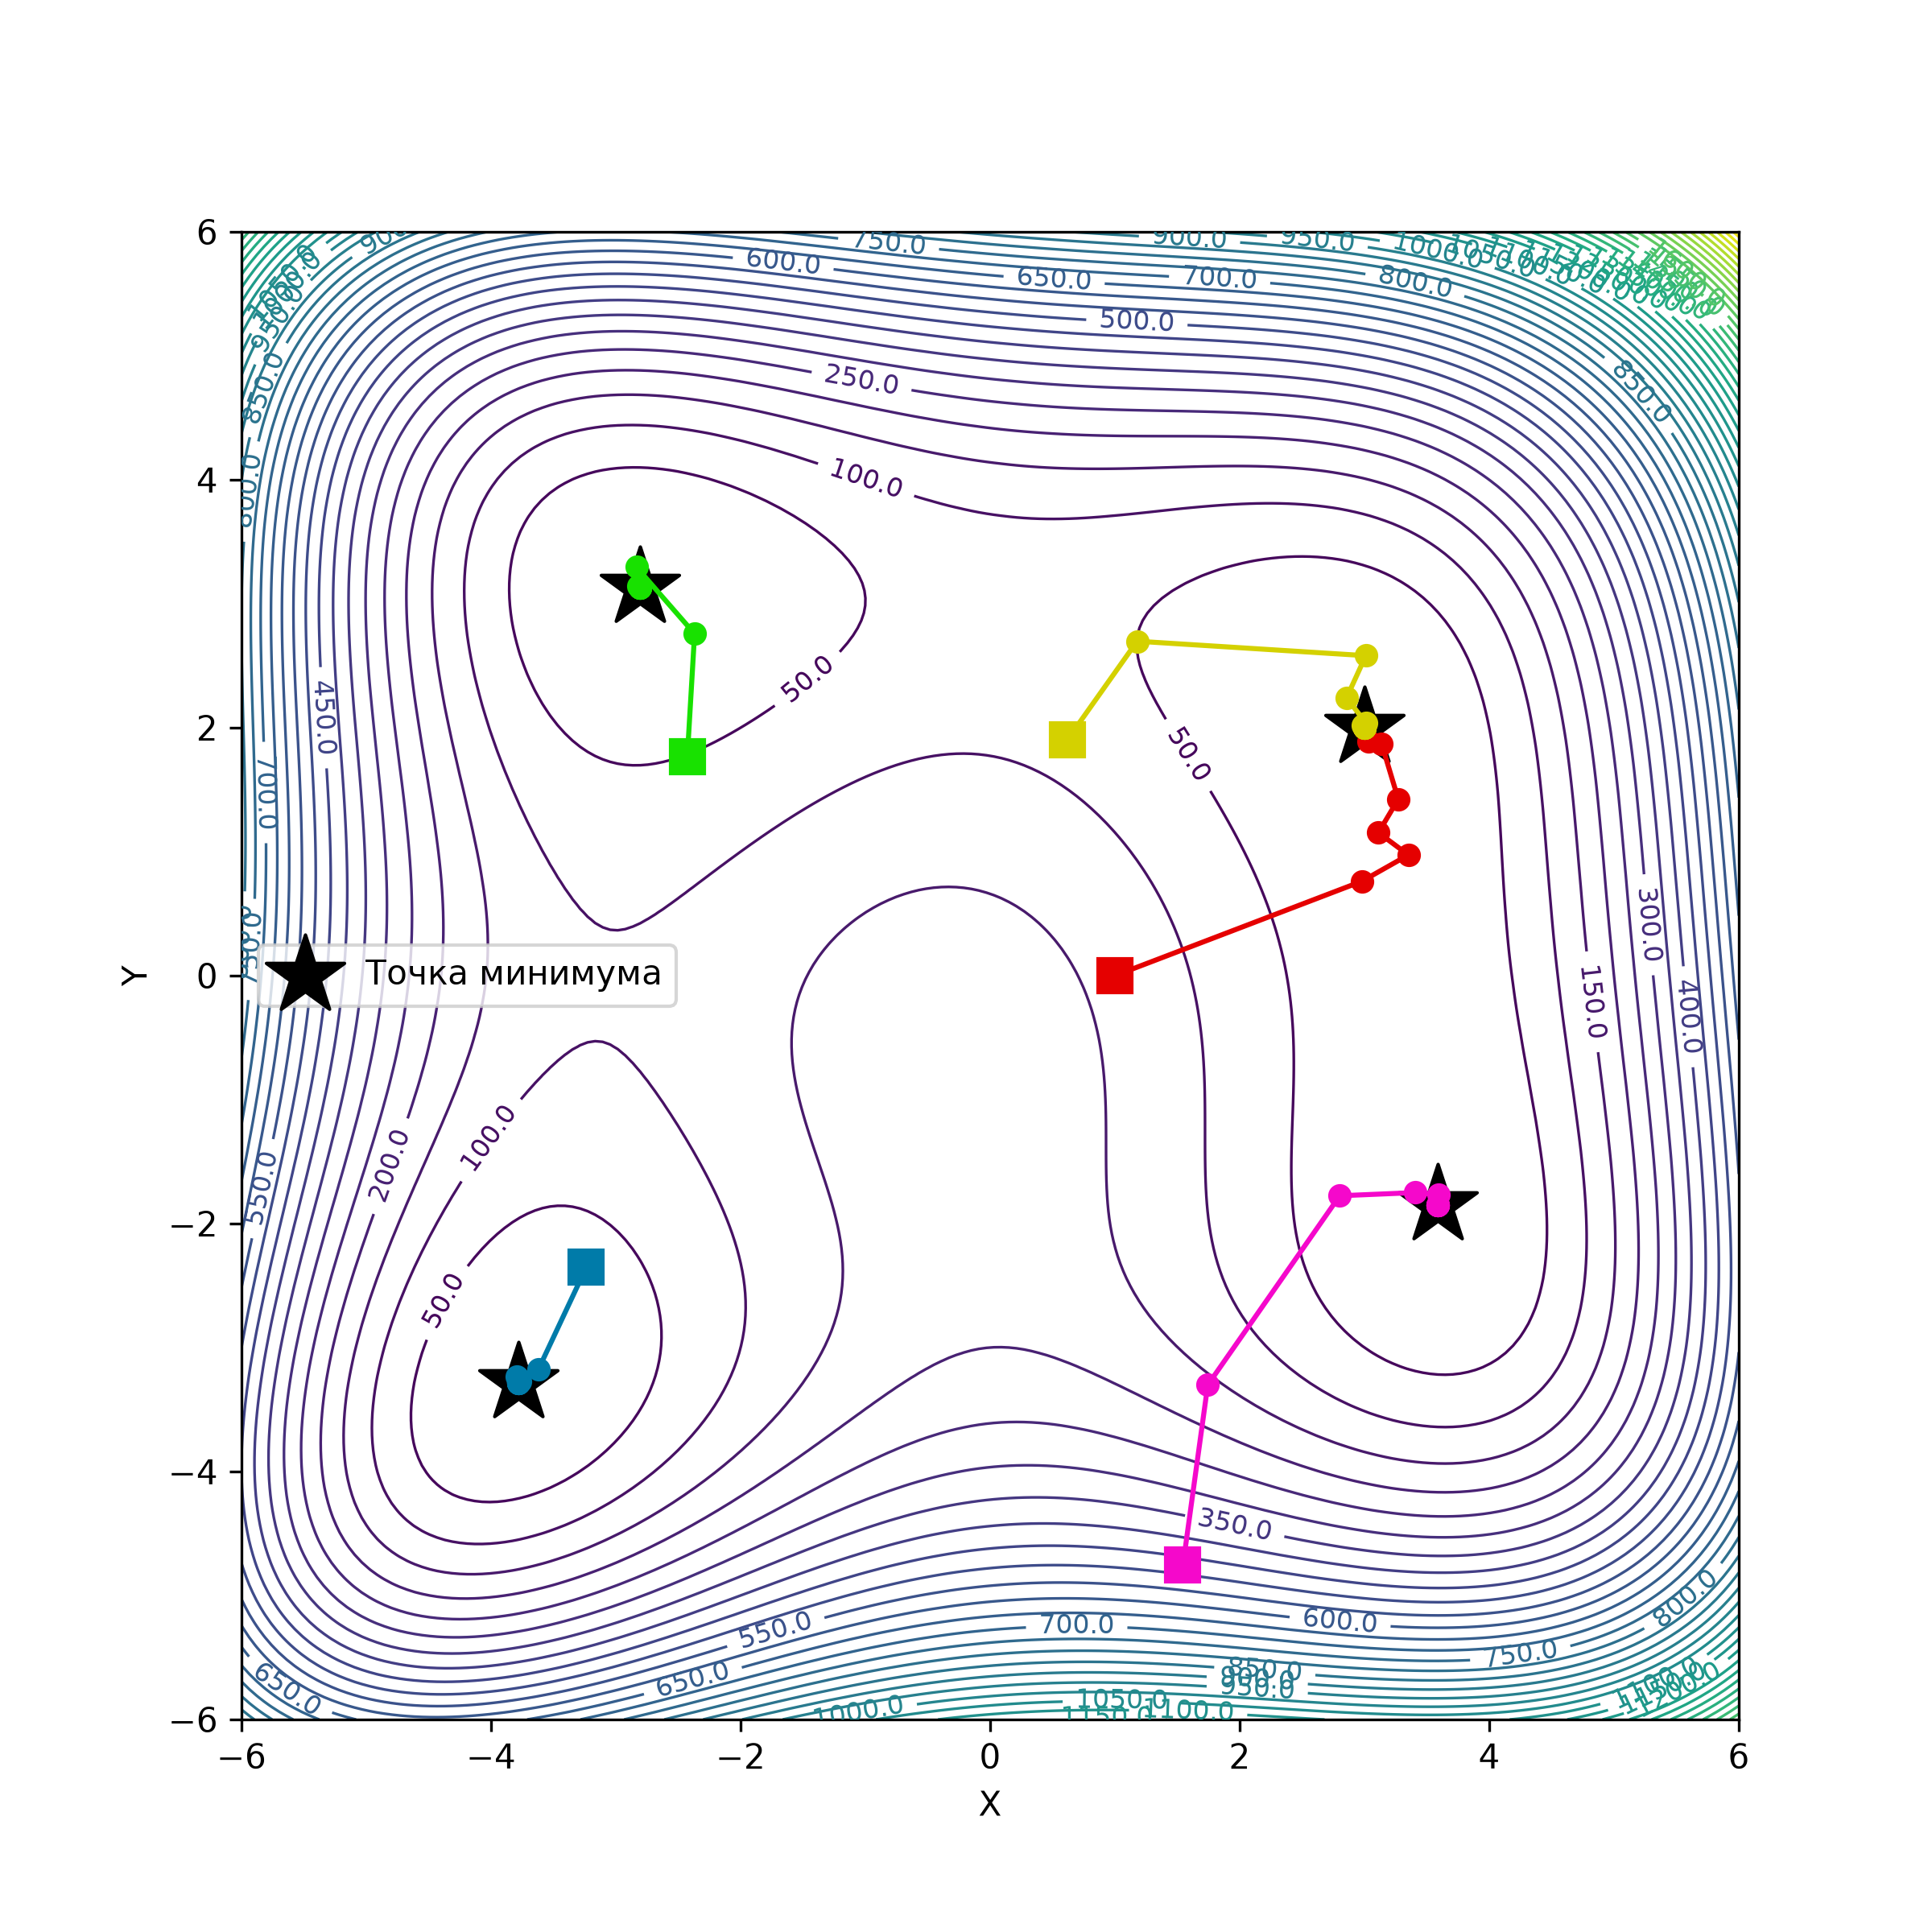
\includegraphics[width=0.3\textwidth]{task3_NewtonCG_Himmelblau function_plot.png}}%
\hfill % <-- Seperation
\subcaptionbox{Powell's Dog Leg}{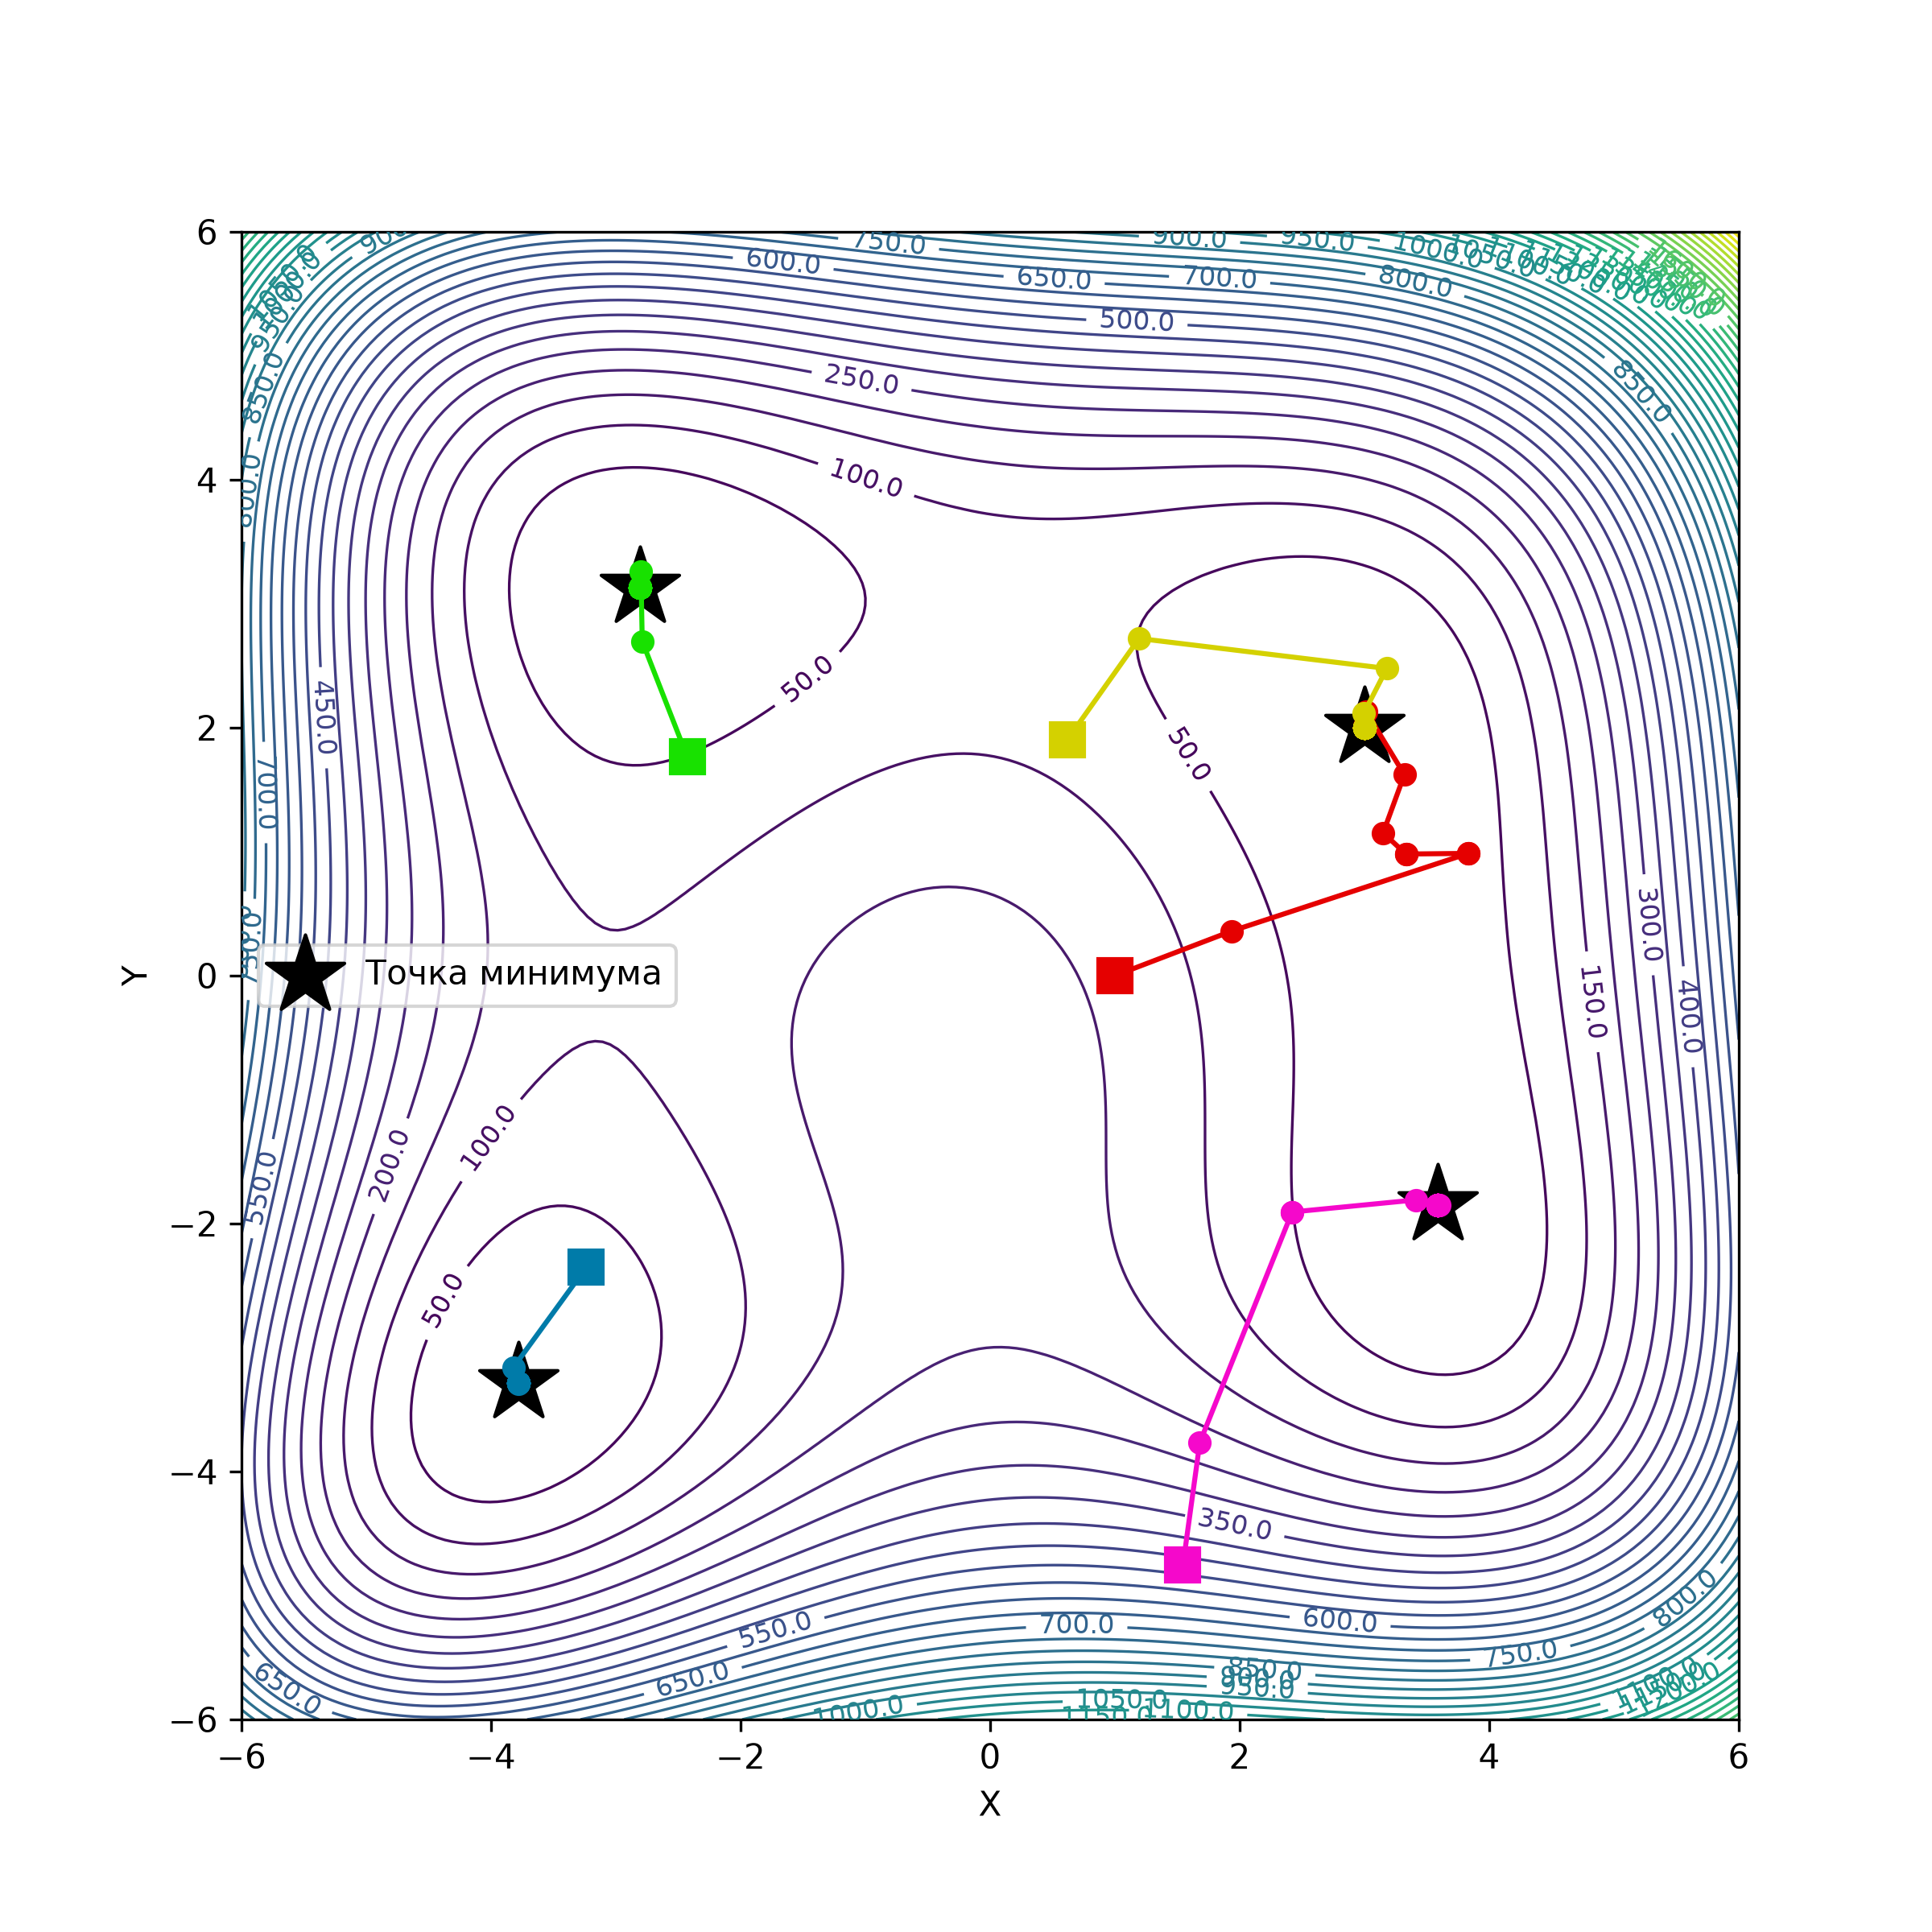
\includegraphics[width=0.3\textwidth]{task3_PowellsDogLeg_Himmelblau function_plot.png}}%
\\ % <-- Line break
\centering
\subcaptionbox{DFP}{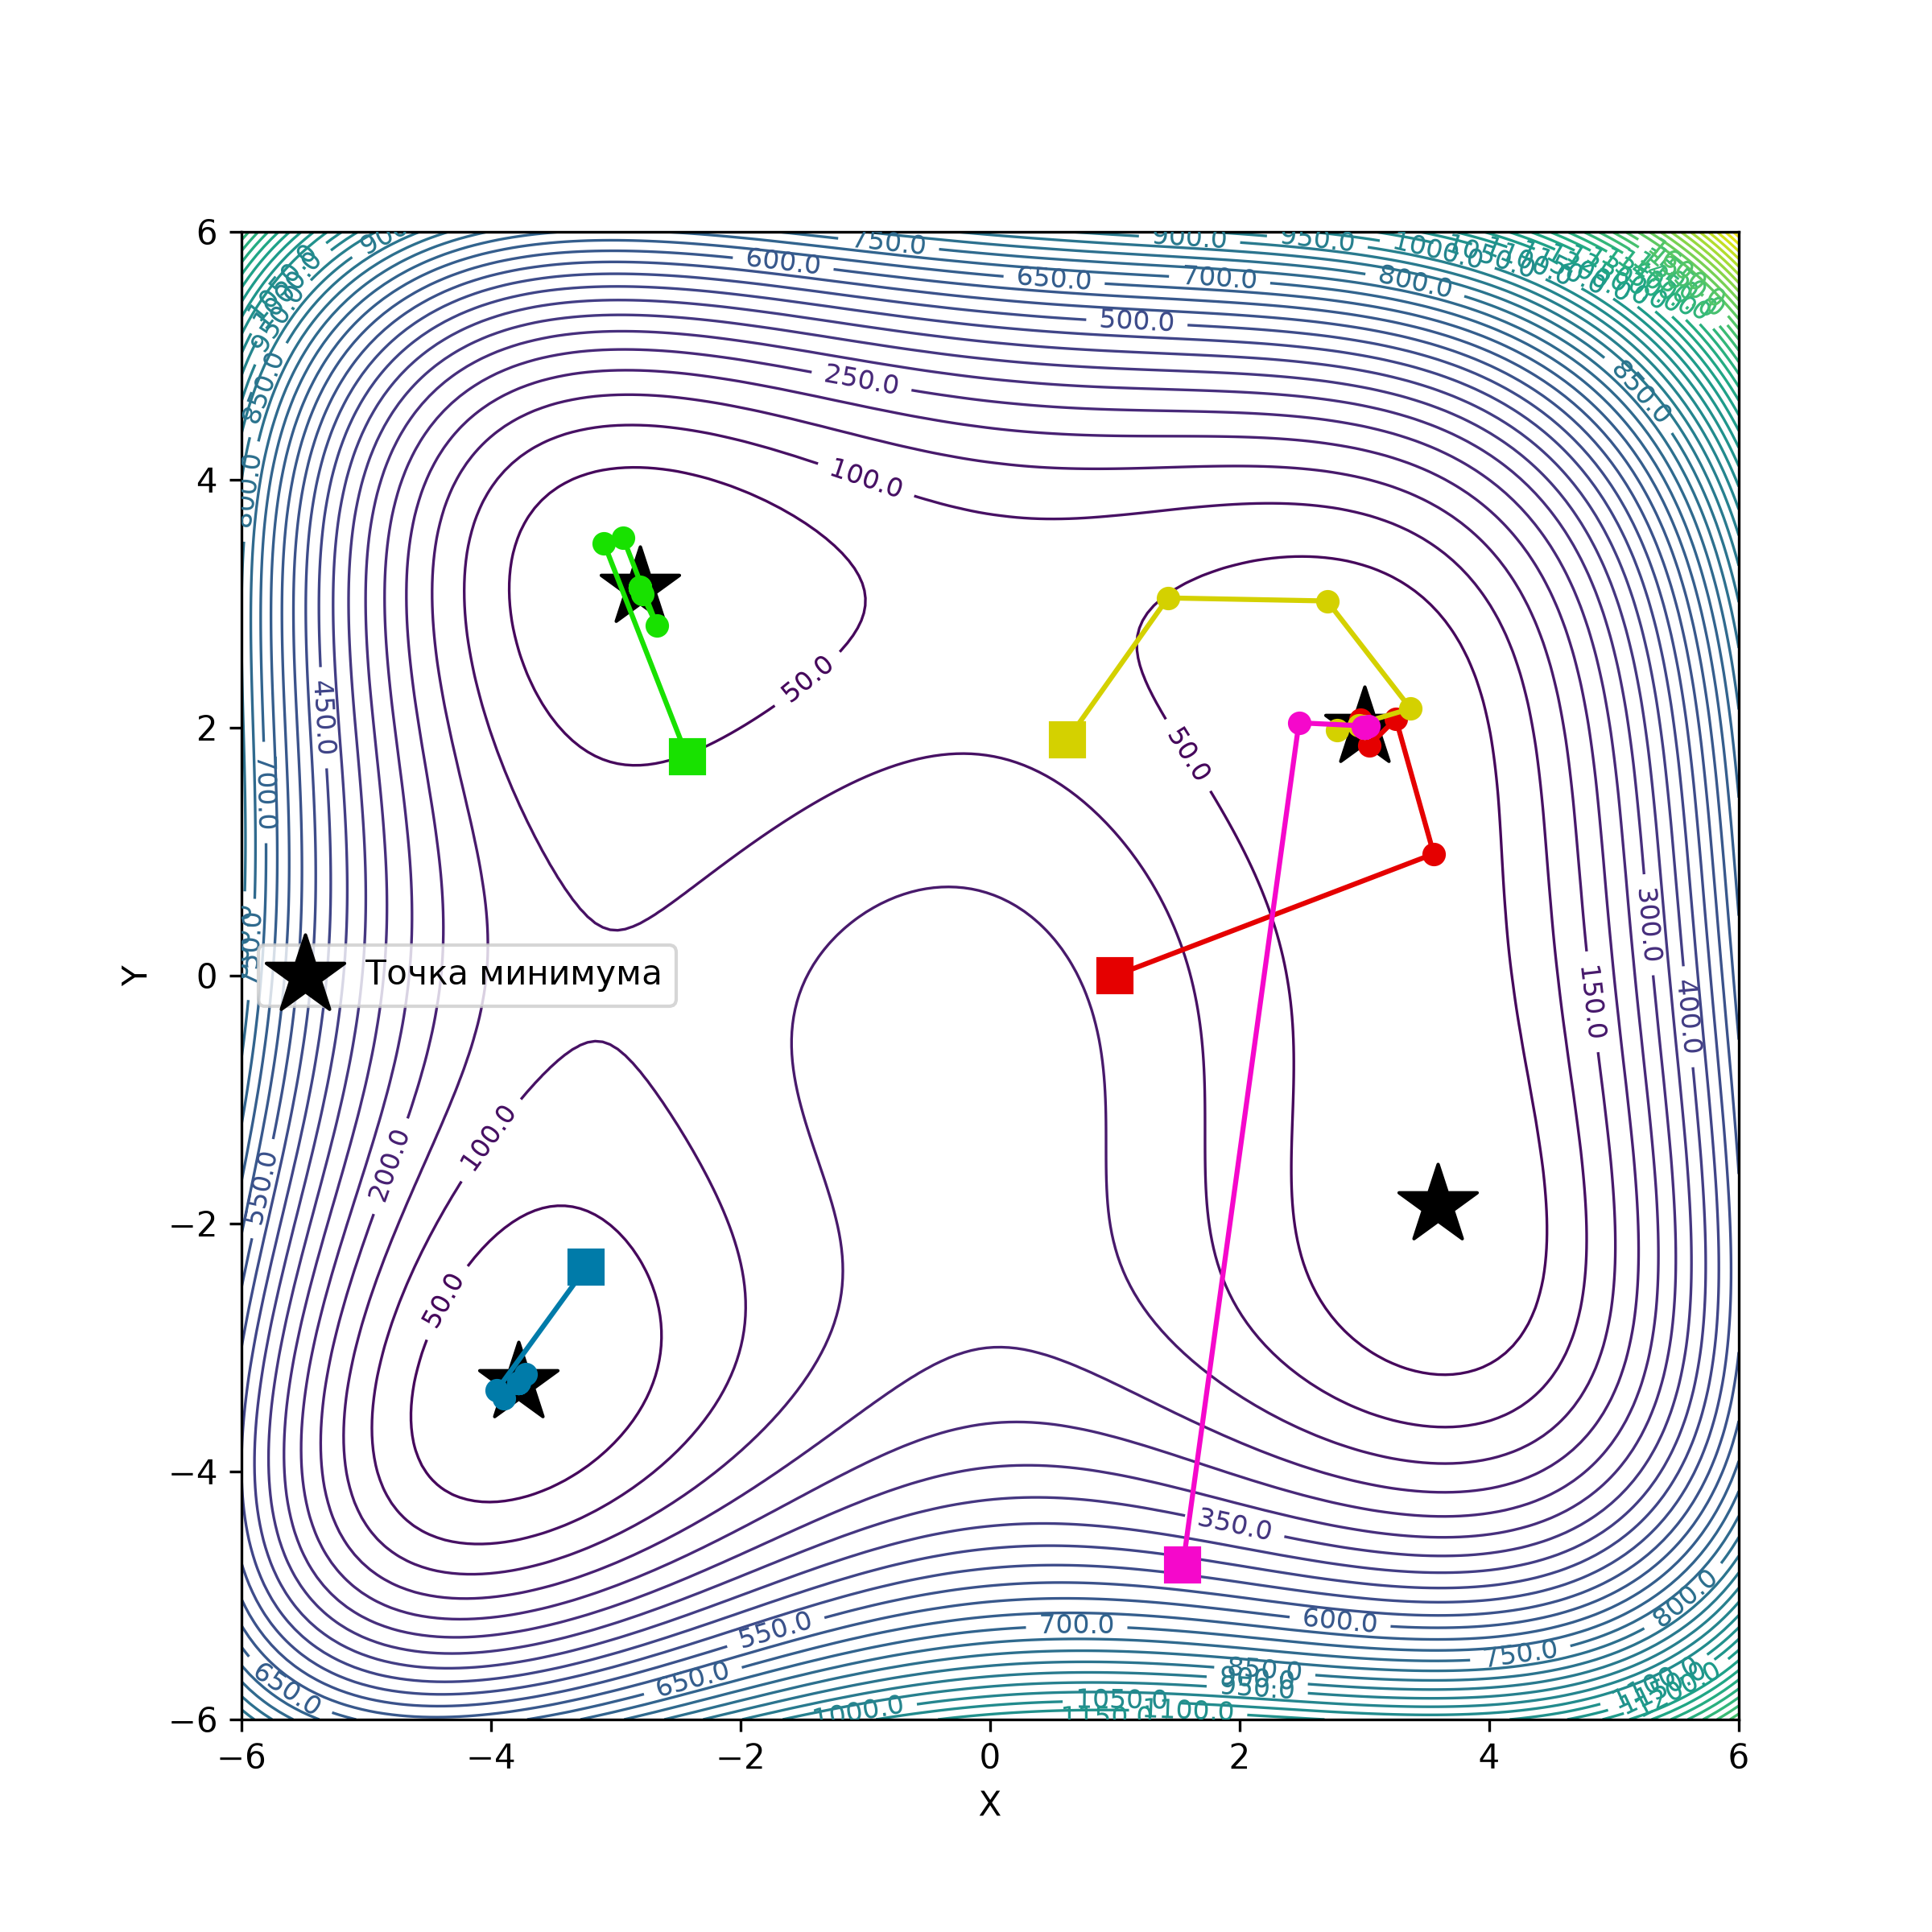
\includegraphics[width=0.3\textwidth]{task3_DFP_Himmelblau function_plot.png}}%
\hfill % <-- Seperation
\subcaptionbox{BFGS}{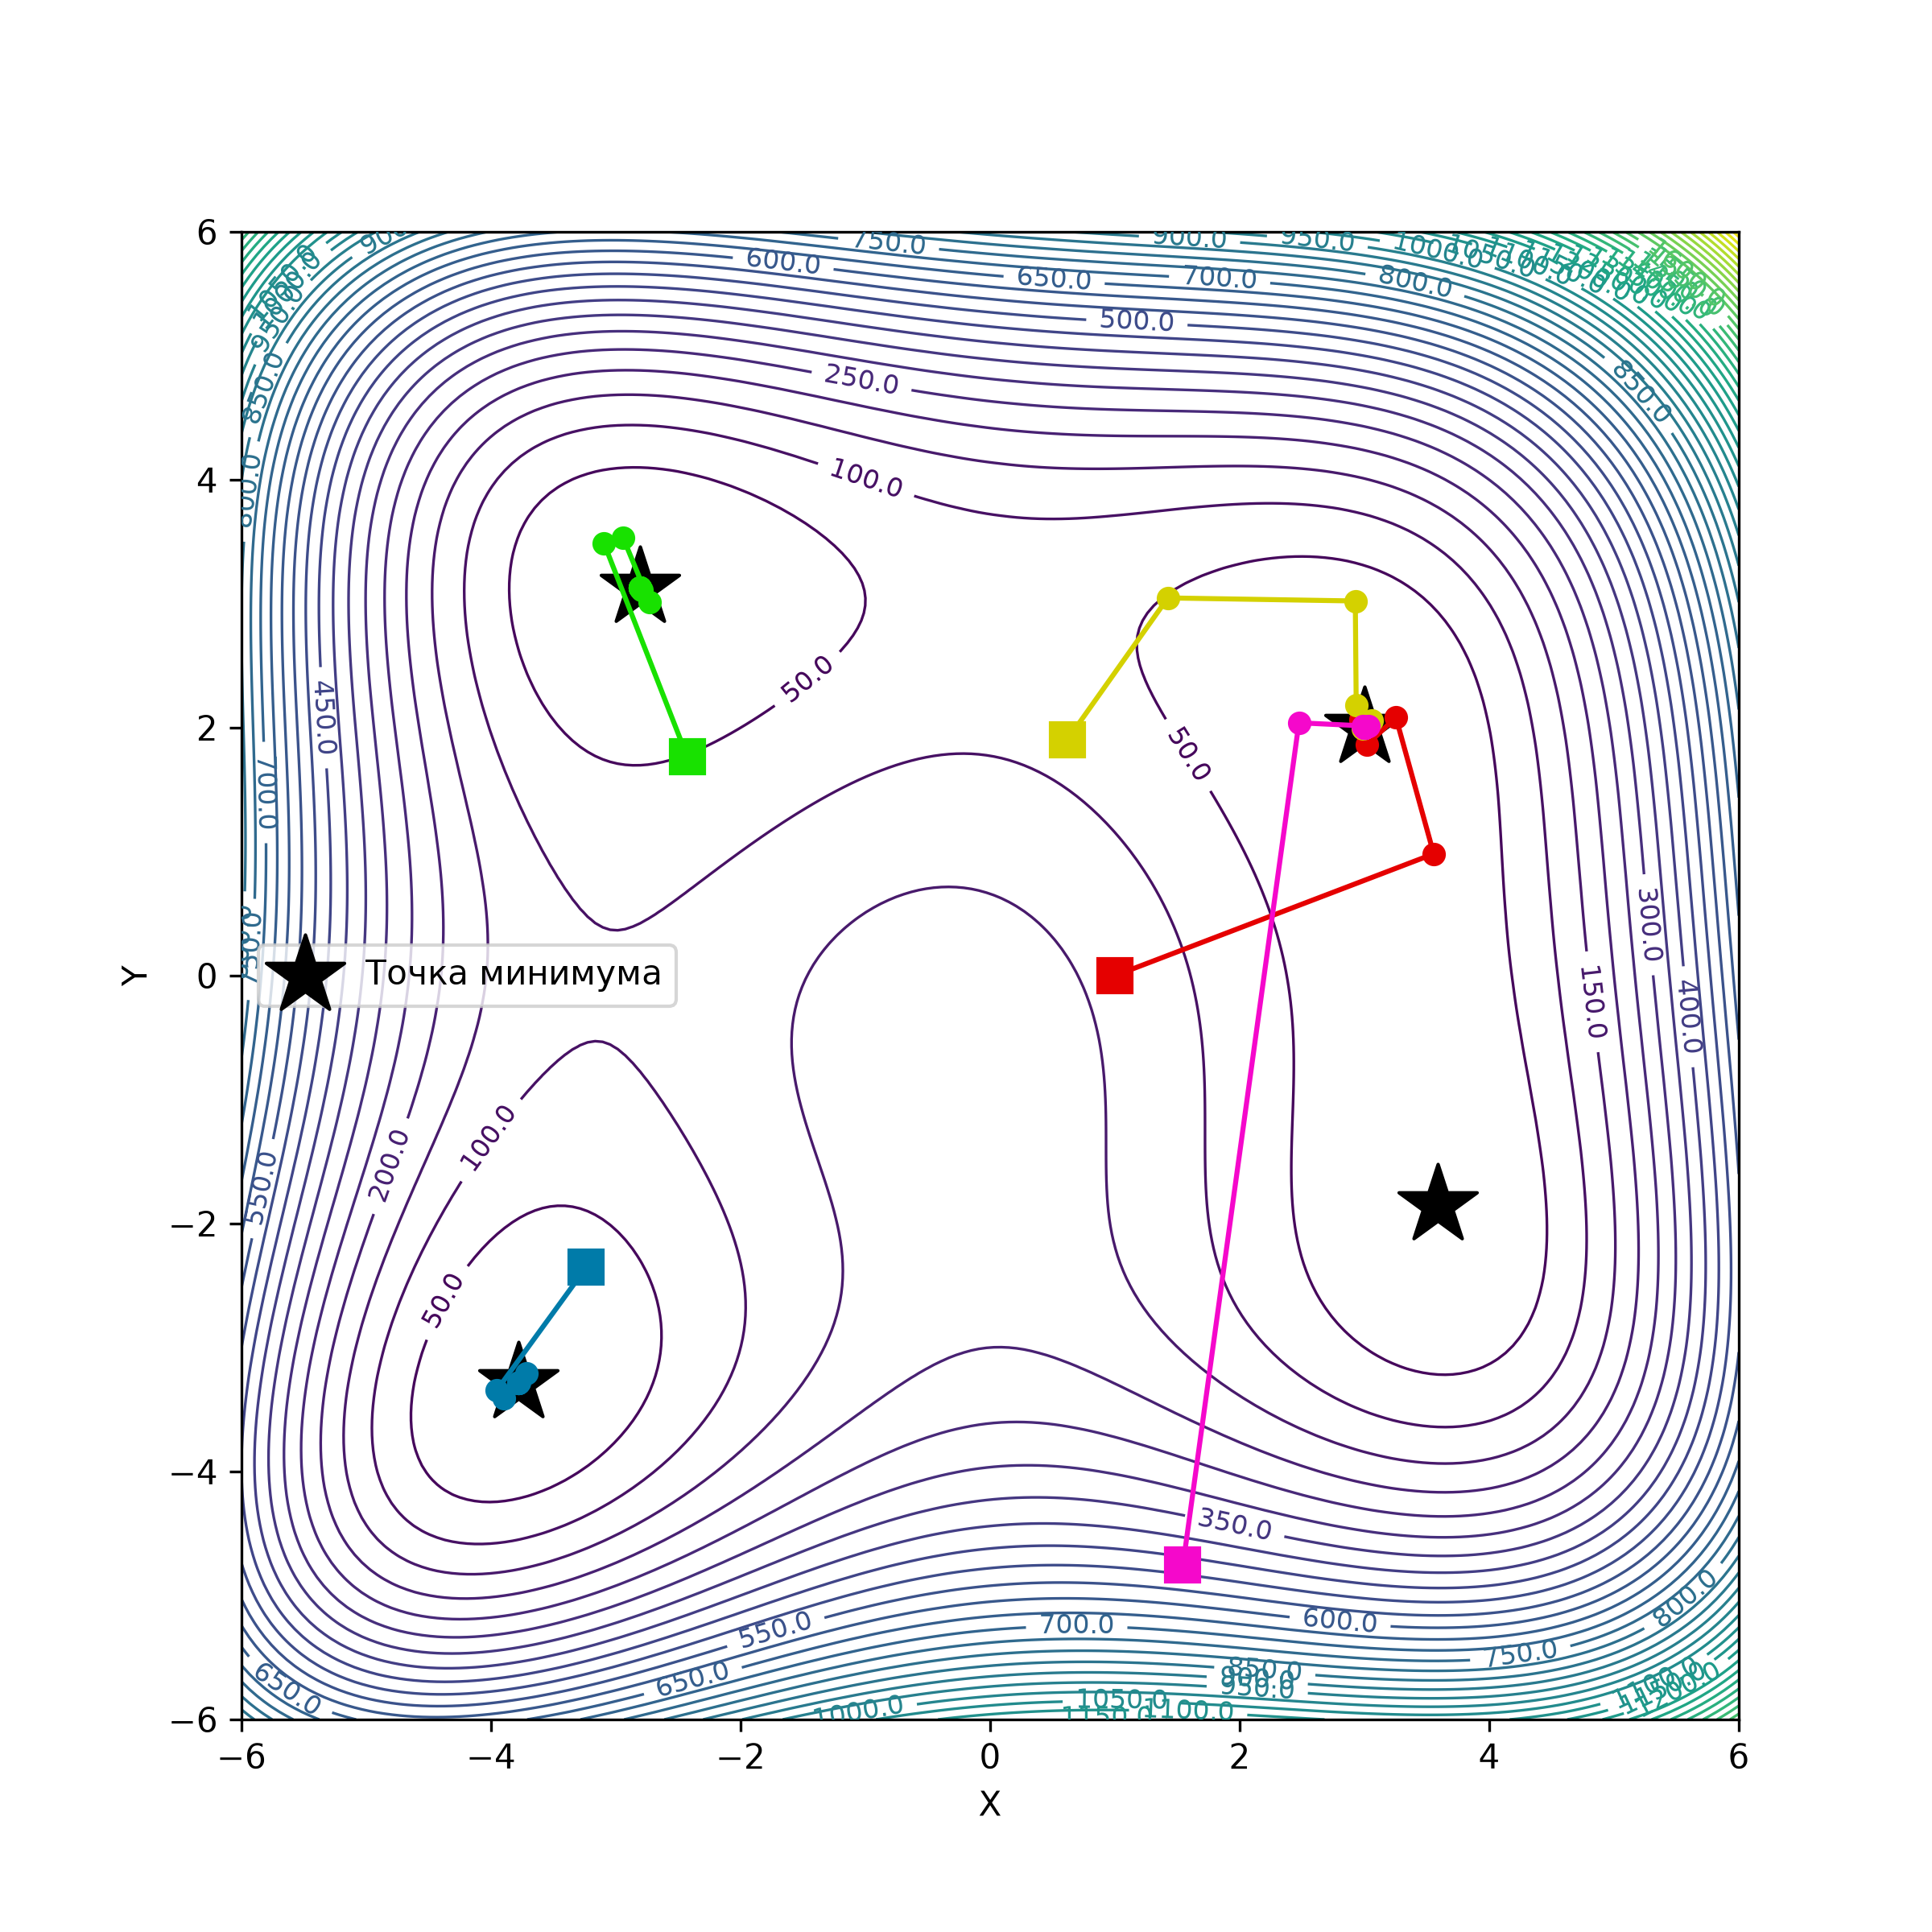
\includegraphics[width=0.3\textwidth]{task3_BFGS_Himmelblau function_plot.png}}%
\hfill % <-- Seperation
\subcaptionbox{L-BFGS}{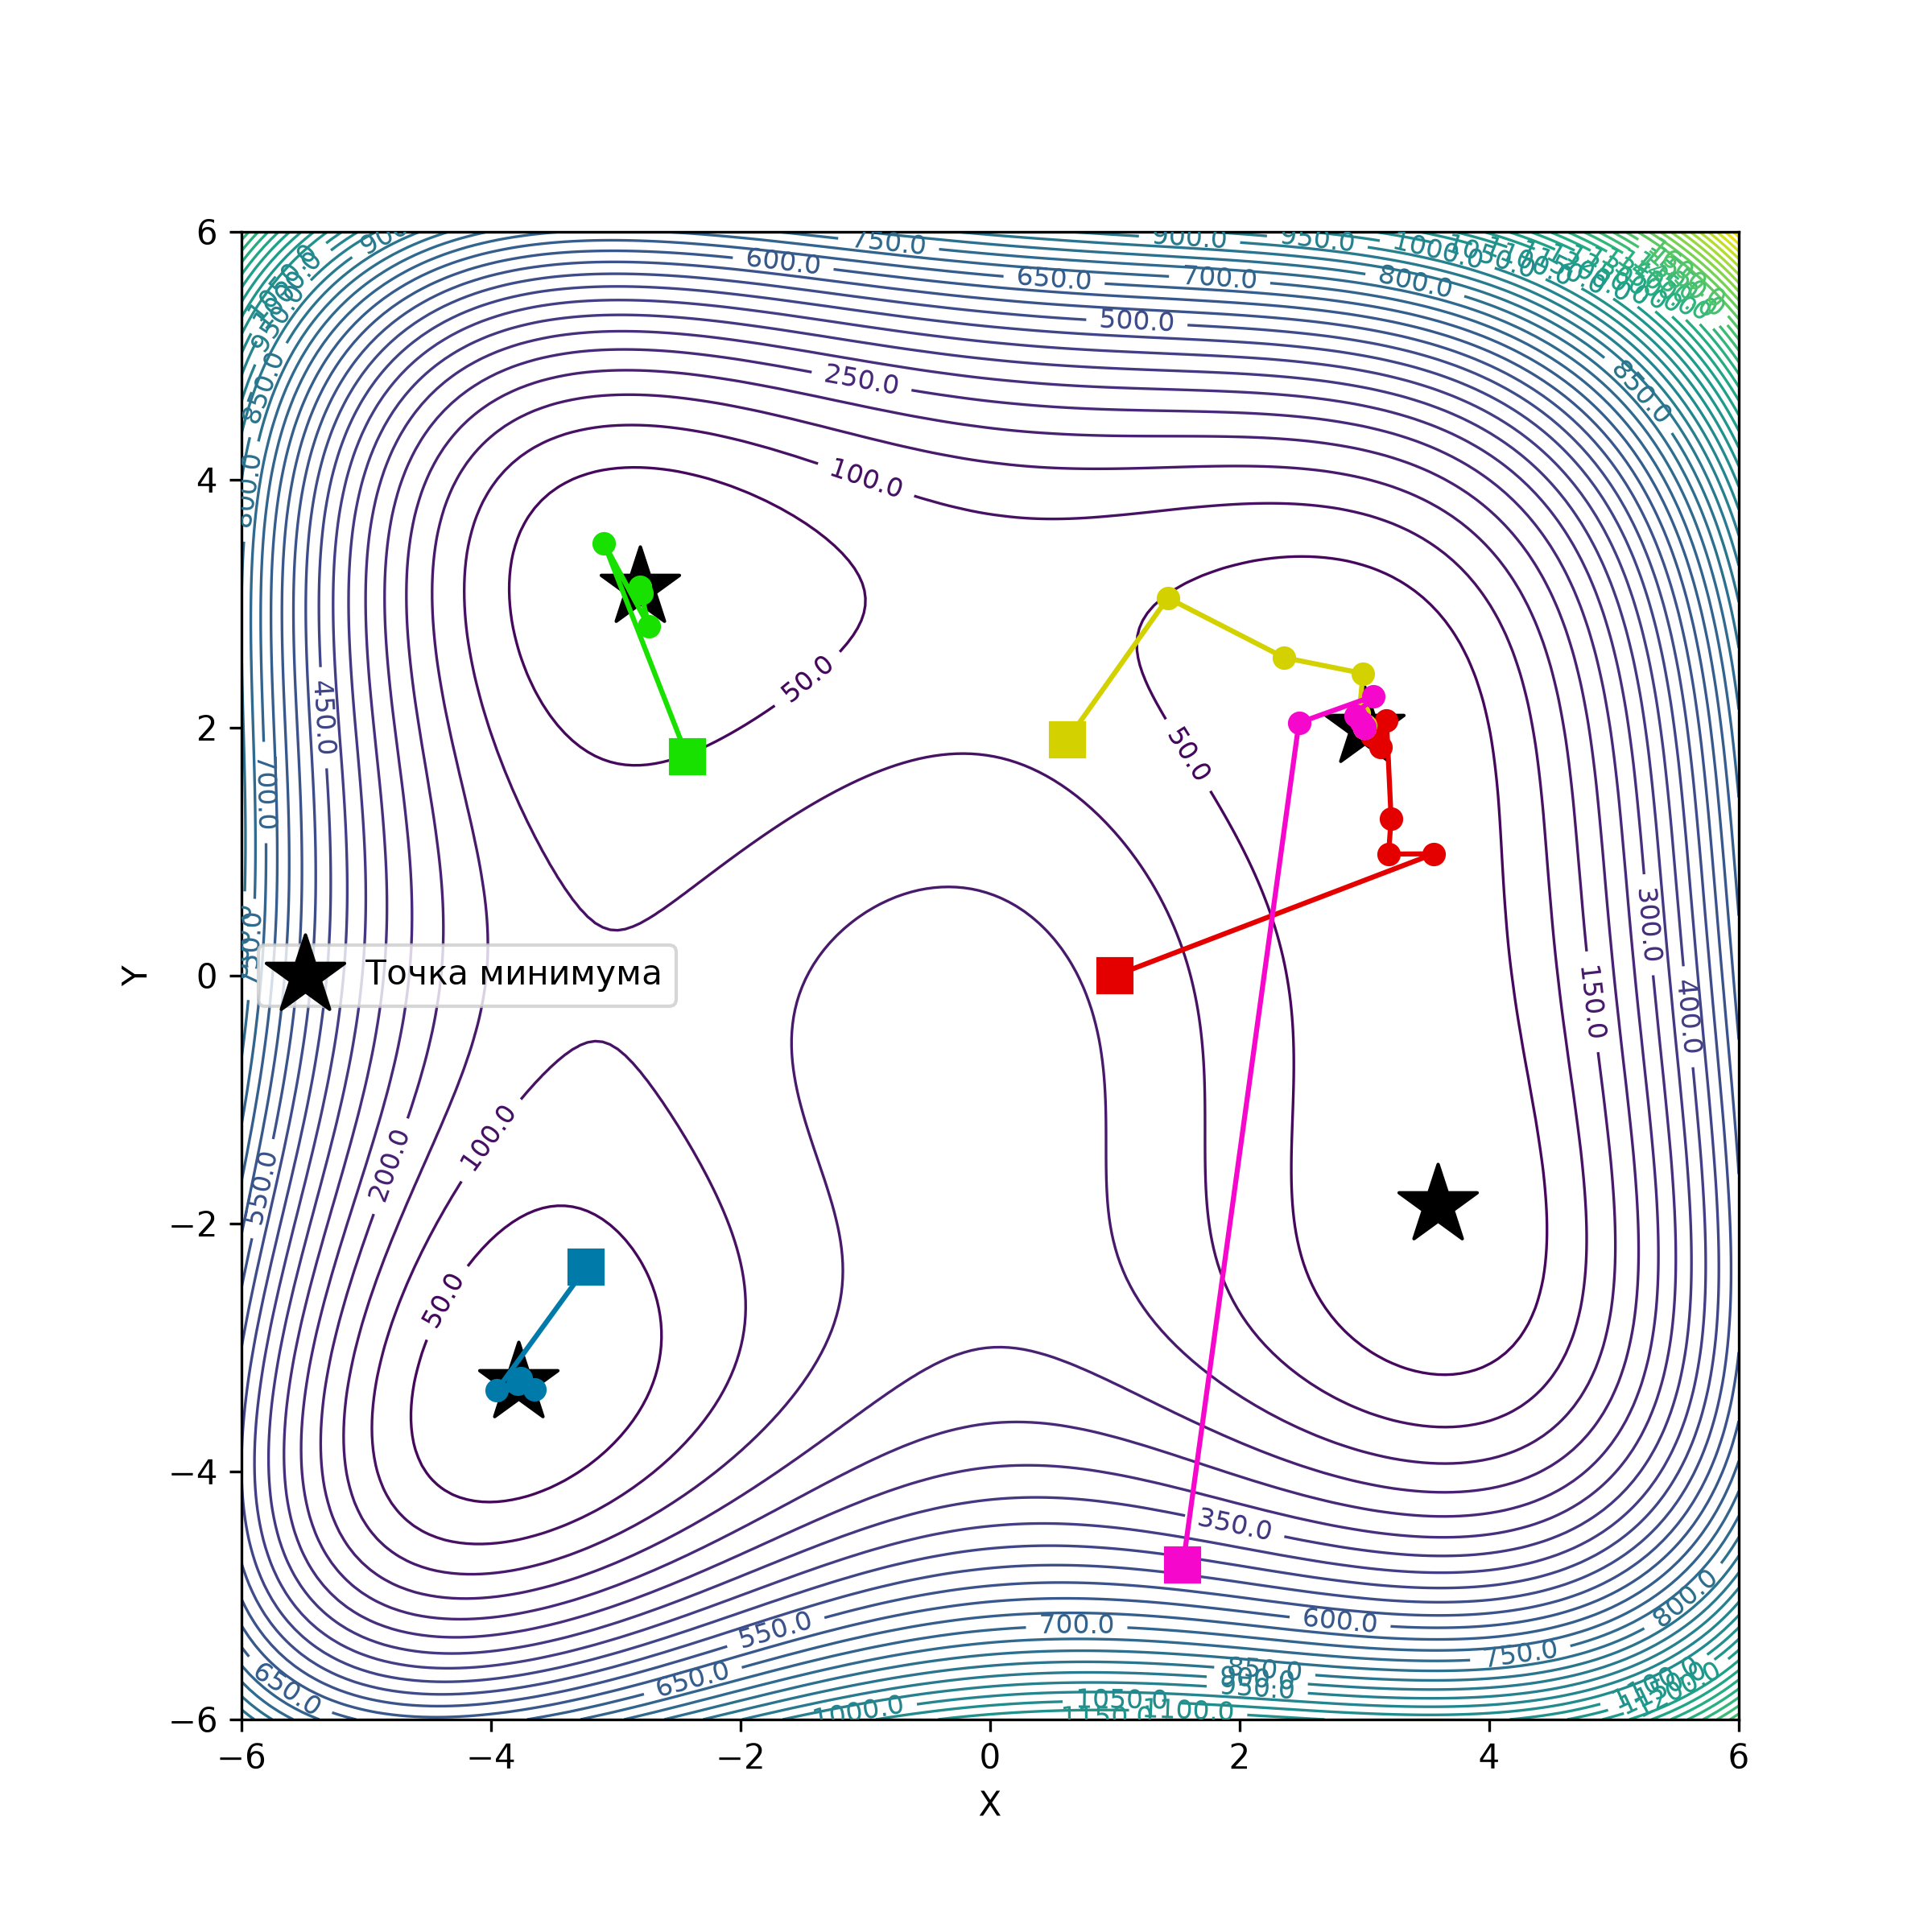
\includegraphics[width=0.3\textwidth]{task3_LBFGS_Himmelblau function_plot.png}}%
\\ % <-- Line break
\caption{Работа оптимизаторов на функции Химмельблау.}
\end{figure}

\begin{figure}[H]
\centering
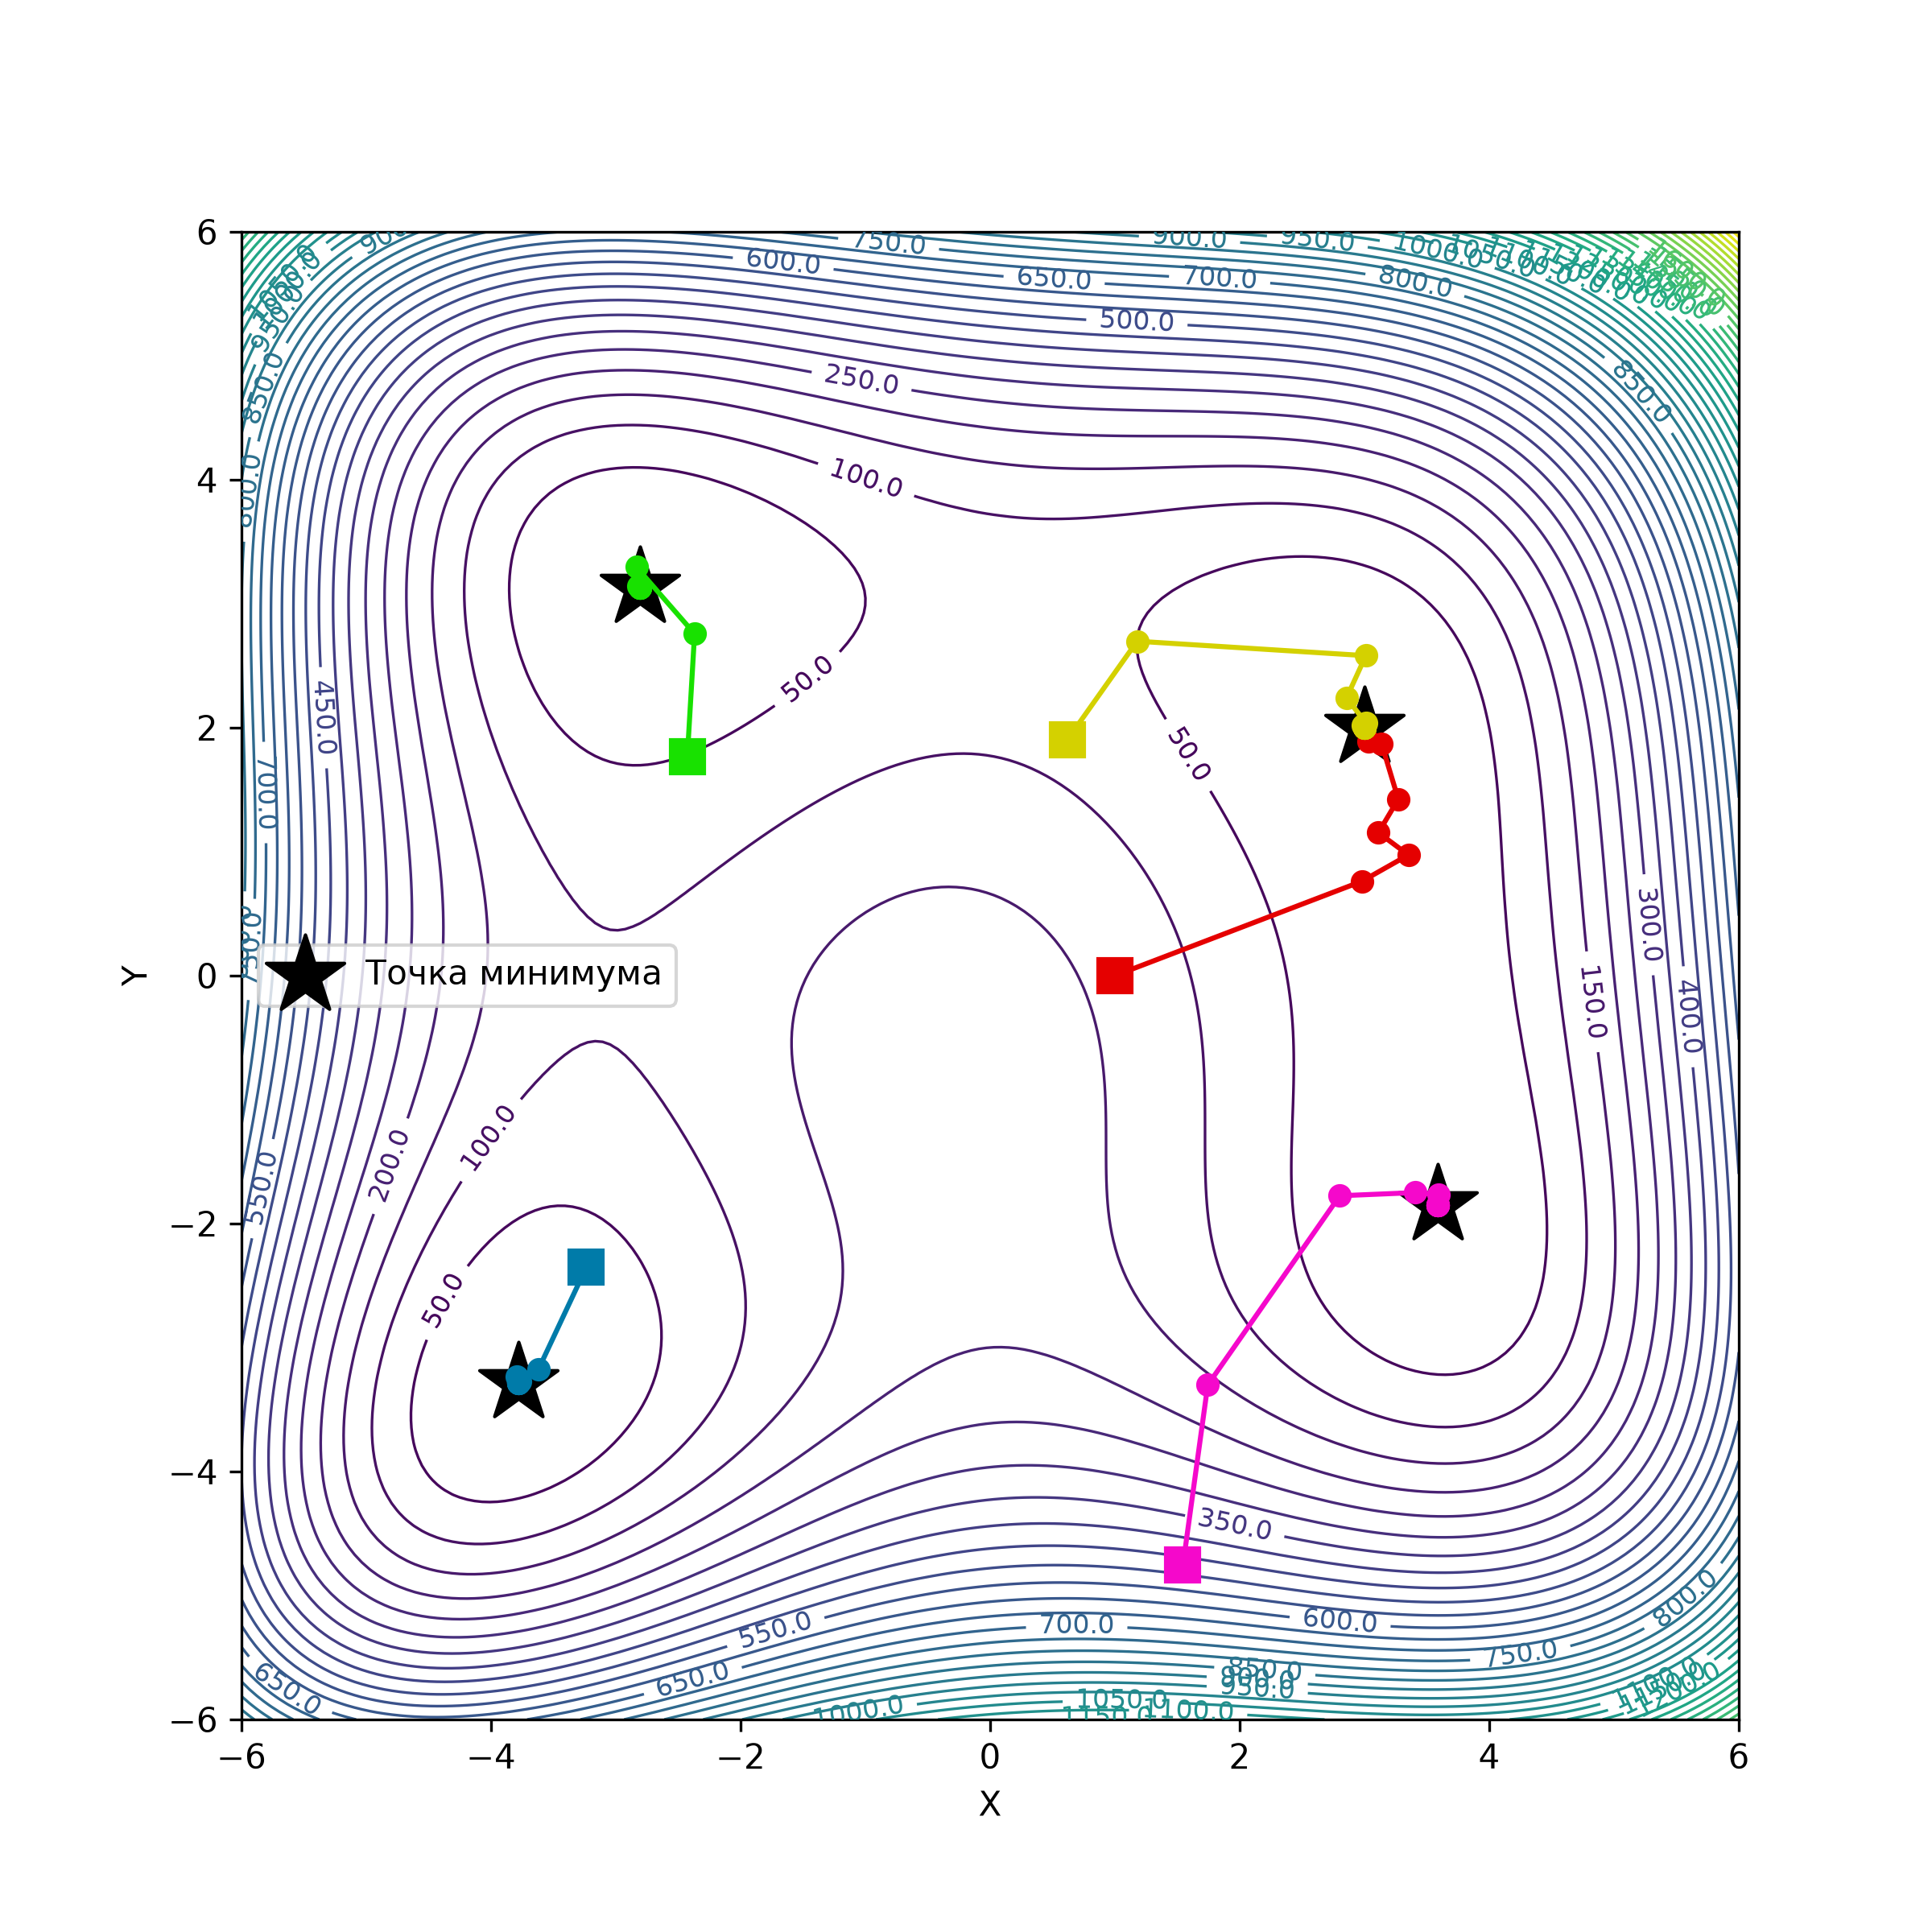
\includegraphics[width=1\textwidth]{task3_NewtonCG_Himmelblau function_plot.png}
\caption{Работа библиотечной NewtonCG на функции Химмельблау.}
\end{figure}

Касательно функции Химмельблау можно сделать те же заключения, что и относительно функции Розенброка, с той лишь разницей, что теперь метод Флетчер-Ривса стабильно сходится к минимуму.

\subsection{Бонус: анализ L-BFGS}

Для анализа особенностей сходимости метода L-BFGS в зависимости от количества хранимых пар была проведена серия опытов над квадратичной функций в пространстве мерности 30 и числом обусловленности $k=10^5$. Получены следующие результаты:

\begin{figure}[H]
\centering
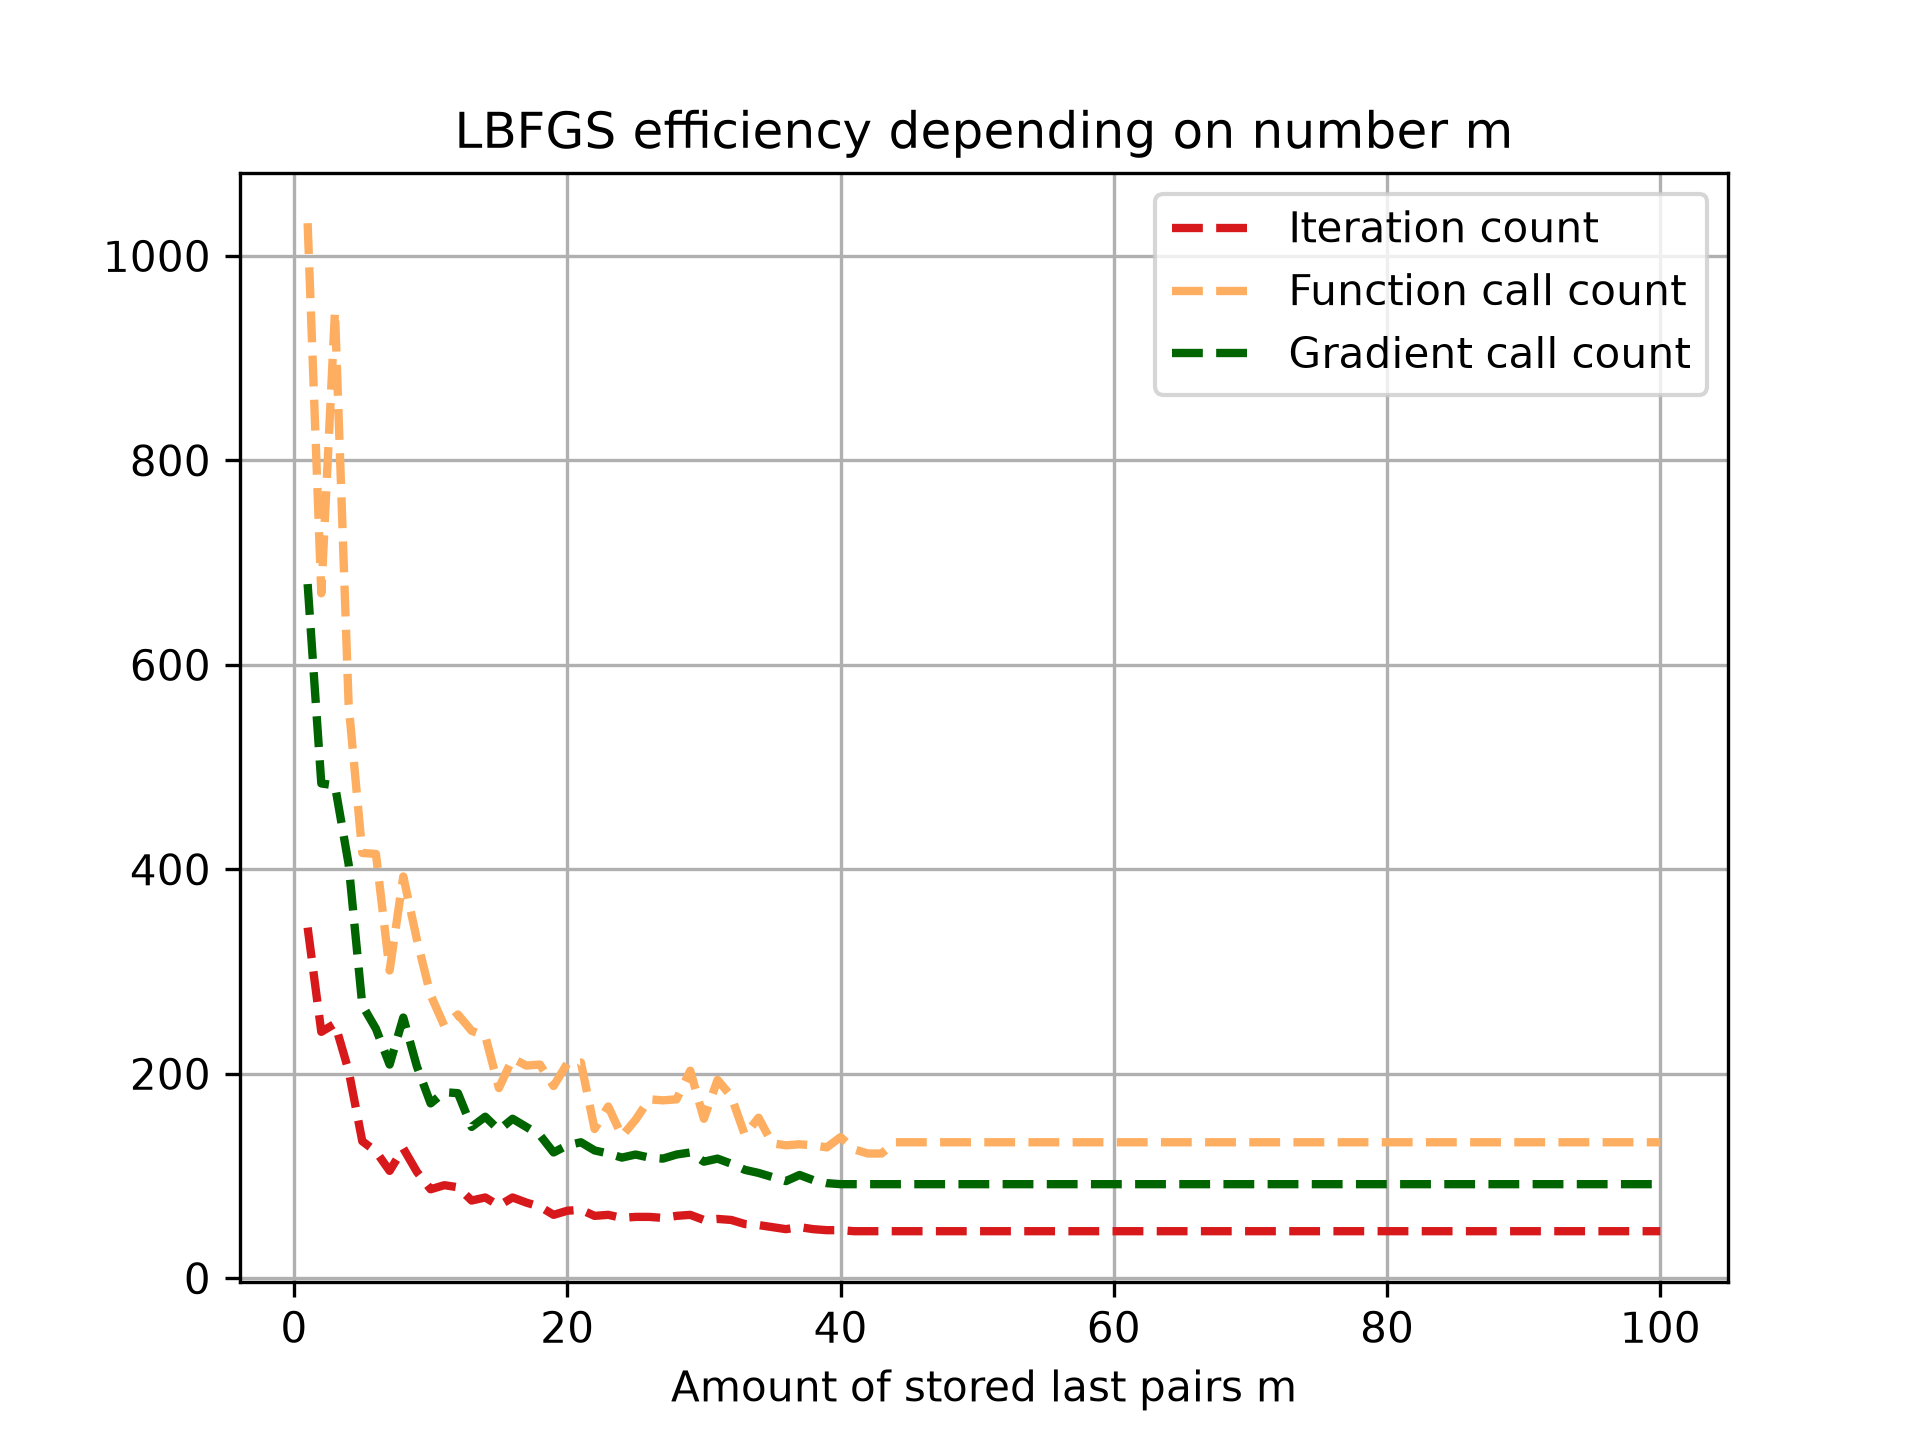
\includegraphics[width=1\textwidth]{task4_plot.png}
\caption{Зависимость числа итераций от количества хранимых пар $m$.}
\end{figure}

Видно, что при увеличении количества хранимых пар число итераций, вызовов функции и вызовов градиента стремится к константе. Также заметно, что при увеличении числа хранимых пар график стабилизируется, причем отклонения исчезают после $m=45$. Это говорит о более эффективной работе алгоритма с увеличением числа хранимых пар.

\section{Выводы и анализ результатов работы}
\begin{itemize}
    \item Были реализованы и исследованы методы сопряженных градиентов, а также ньютоновские и квазинютоновские методы.
    \item  Проведено сравнение собственных реализаций с библиотечной реализацией NewtonCG.
    \item Получены экспериментальные данные работы методов.
    \item  Проведён анализ работы методов при различных конфигурациях оптимизационной задачи на основании полученных данных.
    \item Построены графики, иллюстрирующие работу методов.    
\end{itemize}

\end{document}
